\documentclass[a4paper]{article} 
% \documentclass[a4paper, twocolumn]{article}

%% Language and font encodings
\usepackage[english]{babel}
\usepackage[utf8]{inputenc}
\usepackage[T1]{fontenc}
%% Sets page size and margins
\usepackage[a4paper,top=2cm,bottom=2cm,left=2.5cm,right=2.5cm,marginparwidth=1.75cm]{geometry}
\usepackage{enumitem}
\usepackage{environ}
\usepackage{graphicx}
%% Useful packages
\usepackage{amsmath}
\usepackage{graphicx}
\usepackage{tabularx}
\usepackage{xcolor}
\definecolor{tcdBlue}{RGB}{5, 105, 185}
\usepackage[colorlinks=true,allcolors=.,urlcolor=blue]{hyperref} % allowing hyperlinking of references. You can set the colour of the links or turn the colorlinks to false if no colour preferable. 
\usepackage[numbers]{natbib} % for Vancouver numbering style citation. Remove the [numbers] command for author-year Harvard style referencing. 
\graphicspath{ {./images/} }
%% For numbered lists to follow heading numbering
\NewEnviron{myenum}{
    \begin{enumerate}[label=\thesubsection.\arabic*]
        \BODY
    \end{enumerate}
}

%% For monospace fonts
\def\code#1{\texttt{#1}}

%% optional changes to the style. Comment (Ctrl+/) to remove these options. 
% change font to sans-serif fonts. 
\renewcommand{\familydefault}{\sfdefault}
% Format chapter headings appropriately to include tcd blue. 
\usepackage{titlesec}
\titleformat{\section}[hang]{\normalfont\Large\bfseries\color{tcdBlue}}{\thesection}{1em}{}{}


%% For nomenclature. Comment away if not used. 
% \usepackage{nomencl} % for nomenclature
% \usepackage{etoolbox} % to group nomenclature
% \usepackage{multicol} % for multiple columns in a page/table

\hyphenation{op-tical net-works semi-conduc-tor}

\begin{document}
\title{COMP6845 Report 1}
\author{Antheo Raviel Santosa}
\date{Term 2, 2024}
\maketitle

% \begin{abstract}
%     Input abstract here. The abstract should be short, and contain a summary of what is to be expected in the report. Some key findings is recommended to be highlighted in the abstract.
% \end{abstract}


\tableofcontents % Optional. Remove if unnecessary (or ugly). 
% \input{Addendum/nomenclature} % Optional. Remove if unnecessary. 
\section{Introduction} % (fold)
\label{sec:introduction}

\subsection{Background} % (fold)
\label{sub:background}

\begin{myenum}
    \item Jim's Forensics (JF) have been engaged by Penelope Legal (PL) in relation to proceedings with Caelus Engineering (CE).
    \item On the $14^\text{th}$ of September, 2021, PL instructed JF by letter containing a series of instructions on which we were to proceed.
\end{myenum}

% subsection Background (end)

\subsection{My instructions} % (fold)
\label{sub:my_instructions}

\begin{myenum}
\item As a result of the above engagement, on the $14^\text{th}$ of September, 2021, PL advised me to prepare a report addressing the following issues:
    \begin{enumerate}
        \item \textbf{Question 1 -} Does the data on the laptop provide any indications regarding the reason for its destruction and disposal? If so, what?
        \item \textbf{Question 2 -} Is there any indication of an attempt to "cover tracks", such as deleting or obscuring data?
        \item \textbf{Question 3 - } What additional sources would you want which would aid you in your investigation
    \end{enumerate}
\end{myenum}

% subsection My instructions (end)

\subsection{Provided materials} % (fold)
\begin{myenum}
     \item We are provided the following materials from which we are to base our investigations on:
         \begin{enumerate}
            \item a raw image of the hard disk of Alyx Hamilton's laptop,
            \item a photo of the collection site, and 
            \item profiles of the staff at Caelus Engineering.
         \end{enumerate}
\end{myenum}
\label{sub:provided_materials}

% subsection Provided materials (end)

\subsection{Qualifications} % (fold)
\begin{myenum}
     \item I am a second year computer science student at the University of New South Wales, currently enrolled in the COMP6845 course, otherwise known as \emph{Extended Digital Forensics}.
\end{myenum}
\label{sub:qualifications}

% subsection Qualifications (end)

\subsection{Information relied upon} % (fold)
\label{sub:information_relied_upon}

\begin{myenum}
     \item I have relied upon the following information in the preparation of my report:
         \begin{enumerate}
            \item a letter containing instructions addressed to JF dated $14^\text{th}$ of September, 2021,
            \item the forensic image of the laptop used by Alyx Hamilton,
            \item a photo of the collection site, and 
            \item profiles of the staff at Caelus Engineering.
         \end{enumerate}
\end{myenum}

% subsection Information relied upon (end)

\subsection{Disclaimer} % (fold)
\begin{myenum}
     \item I have made all inquiries which I believe are desirable and appropriate for the purposes of this report. There are no matters of significance which I regard as relevant to my opinions which have been withheld.
     \item This report has been prepared solely for the use of PL. In accordance with the usual practice of JF, I expressly disclaim all responsibility to any other person or entity (other than the Court) for any reliance on the content of this report. This report should not be copied or distributed to any other person or entity, other than in connection with the above matter.
\end{myenum}
\label{sub:disclaimer}

% subsection Disclaimer (end)

\subsection{Assumptions} % (fold)
\begin{myenum}
     
     \item In preparing this report, I have made the following assumptions:
         \begin{enumerate}
            \item the information described in the background section above is accurate, and 
            \item the computers identified by CE, and subsequently imaged, were used by Alyx Hamilton.
         \end{enumerate}
\end{myenum}
\label{sub:assumptions}

% subsection Assumptions (end)

\subsection{Structure of this report} % (fold)
\begin{myenum}
     \item The remaining sections of this report addresses the following:
         \begin{enumerate}
            \item In Section 2, I set out information with respect to Question 1 above;
            \item In Section 3, I set out information with respect to Question 2 above;
            \item In Section 4, I set out information with respect to Question 3 above;
         \end{enumerate}
     \item For convenience, I note that I have organised my findings in the same order as the questions outlined in my letter of instruction. I have also included questions, in some instances paraphrased, from the letter of instruction before presenting my corresponding findings. Additionally, I have referred to the appropriate section number as contained in the letter of instruction in my responses.
\end{myenum}
\label{sub:structure_of_this_report}

% subsection Structure of this report (end)

% section Introduction (end)

% paragraph  (end)
% section Background (end)
 % introduction to the report. 
\section{Question 1: Reason for destruction} % (fold)
\label{sec:question_reason_for_destruction}
\subsection{Procurement and extraction of evidence} % (fold)
\label{sub:procurement_and_extraction_of_evidence}

\subsection{Extraction of evidence} % (fold)
\label{sub:extraction_of_evidence}

% subsection Extraction of evidence (end)
\begin{myenum}
    \item This section describes the method with which the evidence laid out in the rest of this report is procured.
    \item A disk image is a digital replica of the contents of a physical drive, including any unallocated space.
    \item I note that there are no additional cryptographic hashes provided with the disk image, nor is the disk image formatted in a forensically admissible format (such as E01).
    \item I extracted the information presented from this point onwards from the provided disk image using the Autopsy forensics toolkit.
\end{myenum}

% subsection Procurement and extraction of evidence (end)

\subsection{Email} % (fold)
\label{sub:email}

\begin{myenum}
\item \label{item:email} I note the existence of an email from \code{alyx.hamilton@caelusengineering.com.au} sent to the address \code{johndavis5891@gmail.com} at 2020-09-04 16:27:18 AEST with the subject: \emph{"It's done"}. Some notable details include:
    \begin{enumerate}
        \item The body of the email contains only the following line: \emph{"The files are copying over as we speak. What should I do now? Where do I meet you?"}.
        \item The email is found on the \code{\textbackslash\textbackslash Root - Mailbox\textbackslash IPM\_SUBTREE\textbackslash [Gmail]\textbackslash Bin}.
        \item This email is the only correspondence found between Alyx Hamilton and \code{johndavis5891@gmail.com}.
        \item This email is the last email found on the disk image of Alyx Hamilton's laptop
    \end{enumerate}
\end{myenum}

% subsection Email (end)


\subsection{Accessing Google Drive} % (fold)
\label{sub:accessing_google_drive}

\begin{table}
    \caption{Google Drive URLs accessed}\label{tab:google_drive}
    \begin{center}
        \begin{tabular}[c]{|l|l|l|}
            \hline
            \multicolumn{1}{|c|}{\textbf{Date accessed}} & 
            \multicolumn{1}{c|}{\textbf{Title}} &
            \multicolumn{1}{c|}{\textbf{URL}} \\
            \hline
            2020-09-04 14:31:21 AEST & PROJECTS 19:20 - Google Drive & \url{https://drive.google.com/drive/folders/1S7ETsRhUs6hCzgH6o-75pLisyJL1ftPL} \\
            2020-09-04 14:27:57 AEST & Shared Drive - Google Drive & \url{https://drive.google.com/drive/folders/1sinCWRITQJTCD0WmsvRfwGIDsC4HlMvA} \\
            2020-09-04 14:27:55 AEST & Shared with me - Google Drive & \url{https://drive.google.com/drive/shared-with-me} \\
            \hline
        \end{tabular}
    \end{center}
\end{table}

\begin{myenum}
     \item Some of the most web history on the device displays the rapid access of various pages in the Google Suite. These are briefly listed in Table~\ref{tab:google_drive}
\end{myenum}

% subsection Accessing Google Drive (end)

\subsection{Attached USB drives} % (fold)
\label{sub:attached_usb_drives}
\begin{myenum}
    \item Table~\ref{tab:usb-drives} details the make, model, and ID of two external USB drives that are recorded to have been connected to this device, as well as the time they were attached.
\end{myenum}

\begin{table}
    \caption{List of attached external USB drives}\label{tab:usb-drives}
    \begin{center}
        \begin{tabular}[c]{|l|l|l|l|l|}
            \hline

            \multicolumn{1}{|c}{\textbf{No.}} & 
            \multicolumn{1}{|c}{\textbf{Device make}} & 
            \multicolumn{1}{|c}{\textbf{Device model}} & 
            \multicolumn{1}{|c}{\textbf{Device ID}} & 
            \multicolumn{1}{|c|}{\textbf{Date/Time}} \\

            \hline

            1 & SanDisk Corp. & Cruzer Blade & 4C530300831216101192 & 2020-09-04 10:11:55 AEST \\
            2 & SanDisk Corp. & Product: 55A5 & 4C530000050910115114 & 2020-09-04 15:50:09 AEST \\

            \hline
        \end{tabular}
    \end{center}
\end{table}

% subsection Attached USB drives (end)

\subsection{Discussion} % (fold)
\label{sub:discussion}

The email found on 2.2.1 appears to be suspicious from multiple aspects. The most noticeable among which is its cryptic language. Furthermore, the recipient is not an address within Caelus Engineering, nor is it one which otherwise appears in other emails in Alyx Hamilton's mailbox. Lastly, the email is found in the \code{Bin} directory, which indicates attempts at hiding it.

The web activity discussed in 2.3.1 were also found to be within temporal proximity of the email discussed above. They directly precede the web history entry belonging to said email. The site accessed, belonging to "Google Drive" and "Google Docs", are benign, but may be used as a method of exfiltrating data.

Likewise, the external USB devices that are noted to have been connected to the device in 2.4.1 are occurences that are otherwise benign, but may be used as a method of exfiltrating data.

% subsection Discussion (end)

% section Question 1: Reason for destruction (end)
 % background of article or theory
\section{Question 2: Covering tracks} % (fold)

\subsection{Deleted email} % (fold)
\label{sub:deleted_email}
\begin{myenum}
    \item The email discussed previously in 2.2.1 was found on the folder \code{\textbackslash\textbackslash Root - Mailbox\textbackslash IPM\_SUBTREE\textbackslash [Gmail]\textbackslash Bin}, which indicates an attempt at deleting the email.
\end{myenum}

\subsection{Deleted project archives} % (fold)
\label{sub:deleted_project_archives}

\begin{myenum}
    \item ZIP archives containing what appears to be project files appear to have been deleted and are found in the 'Recycle Bin', as can be seen in Figure 4 in the appendix.
\end{myenum}

% subsection Deleted project archives (end)
% subsection Deleted email (end)
 % background of article or theory
\section{Question 3: Encryption} % (fold)
\label{sec:Question 3: Encryption}

\subsection{Introduction} % (fold)
\label{sub:Introduction}

\begin{myenum}
	\item The NIST\footnote{NIST, "encrypt," in Glossary | CSRC. [Online]. Available: https://csrc.nist.gov/glossary/term/encrypt. [Accessed: 22-Jul-2024].} defines "encrypt" as to "cryptographically transform data to produce cipher text".
		\begin{enumerate}
			\item The NIST\footnote{NIST, "cryptography," in Glossary | CSRC. [Online]. Available: https://csrc.nist.gov/glossary/term/cryptography. [Accessed: 22-Jul-2024]} further defines "cryptography" as "the discipline that embodies the principles, means, and methods for the transformation of data in order to hide their semantic content, prevent their unauthorized use, or prevent their undetected modification".
			\item The NIST\footnote{NIST, "cipher text," in Glossary | CSRC. [Online]. Available: https://csrc.nist.gov/glossary/term/cipher\_text. [Accessed: 22-Jul-2024]} further defines "cipher text" as "data in its encrypted form".
		\end{enumerate}
	\item Encryption can therefore be defined as the transformation of data in order to ensure its secrecy and integrity.
	\item Encryption is a virtually ubiquitous feature of modern computing technology, as its nature of providing secrecy has a wealth of uses, whether benign (such as protecting one's financial information when performing a transaction online) or malicious (such as obscuring evidence of illegal activities).
\end{myenum}
% subsection Introduction (end)

\subsection{Network encryption} % (fold)
\label{sub:Network encryption}

\begin{myenum}
	\item A pcap, or \emph{packet capture} file, is a file which stores network packet data. Such a file is typically procured by capturing the packets which passes through a device (note that this does not necessarily mean that every packet captured involves said device). Such a file logs all network communication that said device "hears".
		\begin{enumerate}
			\item A "packet" is a small segment of a larger message, which are sent through computer networks, and are recombined by the recipient to obtain the whole message.\footnote{Cloudflare, "What is a Packet?" Cloudflare. Available: https://web.archive.org/web/20240622023826/https://www.cloudflare.com/learning/network-layer/what-is-a-packet/. [Accessed: 22-Jul-2024].}
		\end{enumerate}
	\item JF is provided the pcap file procured from Alyx Hamilton's laptop by CE. 
	\item A cryptographic hash (using the MD5 algorithm) is provided alongside the pcap file. The calculated hash of the pcap file appears to match the provided hash, as can be seen in Figure~\ref{pcap_verification}. Assuming that the integrity of the file containing the provided hash is maintained, this means that the pcap file has not been tampered with throughout the span of time between the calculation of the provided hash and the time of verification.
	\item Secure Sockets Layer (SSL), as well as its successor, Transport Layer Security (TLS), are protocols for encrypting, securing, and authenticating communications that take place on the internet.\footnote{Cloudflare, "How does SSL work?" Cloudflare. [Online]. Available: https://www.cloudflare.com/learning/ssl/how-does-ssl-work/. [Accessed: 22-Jul-2024].} It is used to ensure the secrecy and authenticity of communication over the internet.
	\item Because the pcap file contains packets encrypted using SSL, a log of the SSL keys necessary to decrypt them is also provided to JF by CE. A cryptographic hash of the log is also provided, and the calculated hash of the log file appears to match that of the provided hash, as can be seen in Figure~\ref{ssl_key_log_verification}. Similar to the pcap file, this means that the pcap file has not been tampered with throughout the span of time between the calculation of the provided hash and the time of verification, assuming that the integrity of the file containing the provided hash is maintained.
	\item Wireshark is a network traffic analyser.\footnote{Wireshark Foundation, "Wireshark," GitLab. [Online]. Available: https://gitlab.com/wireshark/wireshark. [Accessed: 22-Jul-2024].} It is a tool that can be used to capture packets from the host device's network interface, creating a pcap file, and analysing pcap files.
		\begin{enumerate}
			\item The pcap file can be accessed in Wireshark by clicking \texttt{File > Open}  on the top menu bar, and then selecting the file from the resulting file explorer dialog.
			\item After opening the pcap file, the SSL key log can be imported by selecting \texttt{Edit > Preferences} on the top menu bar, selecting \texttt{Protocols > TLS} on the preferences menu, and then clicking the the \texttt{Browse} button underneath \texttt{(Pre)-Master-Secret log filename} and selecting the SSL key log file, as can be seen in Figure~\ref{importing_ssl_key_log}.
		\end{enumerate}
	\item Quick UDP Internet Connections (QUIC) is an encrypted-by-default transport protocol originally developed by Google\footnote{A. Ghedini, "The Road to QUIC," Cloudflare Blog. [Online]. Available: https://blog.cloudflare.com/the-road-to-quic. [Accessed: 22-Jul-2024].} that is supported by the Google Chrome web browser, beginning small-scale deployments of the original implementation, gQUIC in 2013, and eventually default-enabling its successor, IETF QUIC in 2021 with Chrome 93.\footnote{Chromium Project, "QUIC, a multiplexed transport over UDP," Chromium. [Online]. Available: https://www.chromium.org/quic/. [Accessed: 22-Jul-2024].}
	\item I note that the version of Google Chrome running on Alyx Hamilton's laptop is 84. This can be found by extracting the list of DLLs from Google Chrome processes found on the memory dump using Volatility, as can be seen in Figure~\ref{chrome_version}.
	 Two points of observation can be drawn from this:
		\begin{enumerate}
			\item It does not appear to be possible to decrypt the QUIC packets sent to and from Google Chrome in the provided pcap file, because the export of QUIC secrets is only available on version 89 onwards of Google Chrome.\footnote{Wireshark Foundation, "The TLS/QUIC sessions can't be decrypted," GitLab. [Online]. Available: https://gitlab.com/wireshark/wireshark/-/issues/17111. [Accessed: 22-Jul-2024].}
			\item It appears that the use of QUIC is manually enabled on the Google Chrome browser running on Alyx Hamilton's laptop, as the protocol is only enabled by default from version 93 onwards of Google Chrome.
		\end{enumerate}
\end{myenum}

% subsection Network encryption (end)

% section Question 3: Encryption (end)
 % background of article or theory
% \input{3_method/method} % methodology
% \input{4_results/results} % elaborating on the results
% \input{5_analysis/analytics} % analyse the data. Can be combined with the results section to form one combined section. 
% \input{6_conclusion/conclusion}
\section{Appendix}
\subsection{Figures} % (fold)
\label{sec:Figures}

\begin{figure}[H]
    \centering
    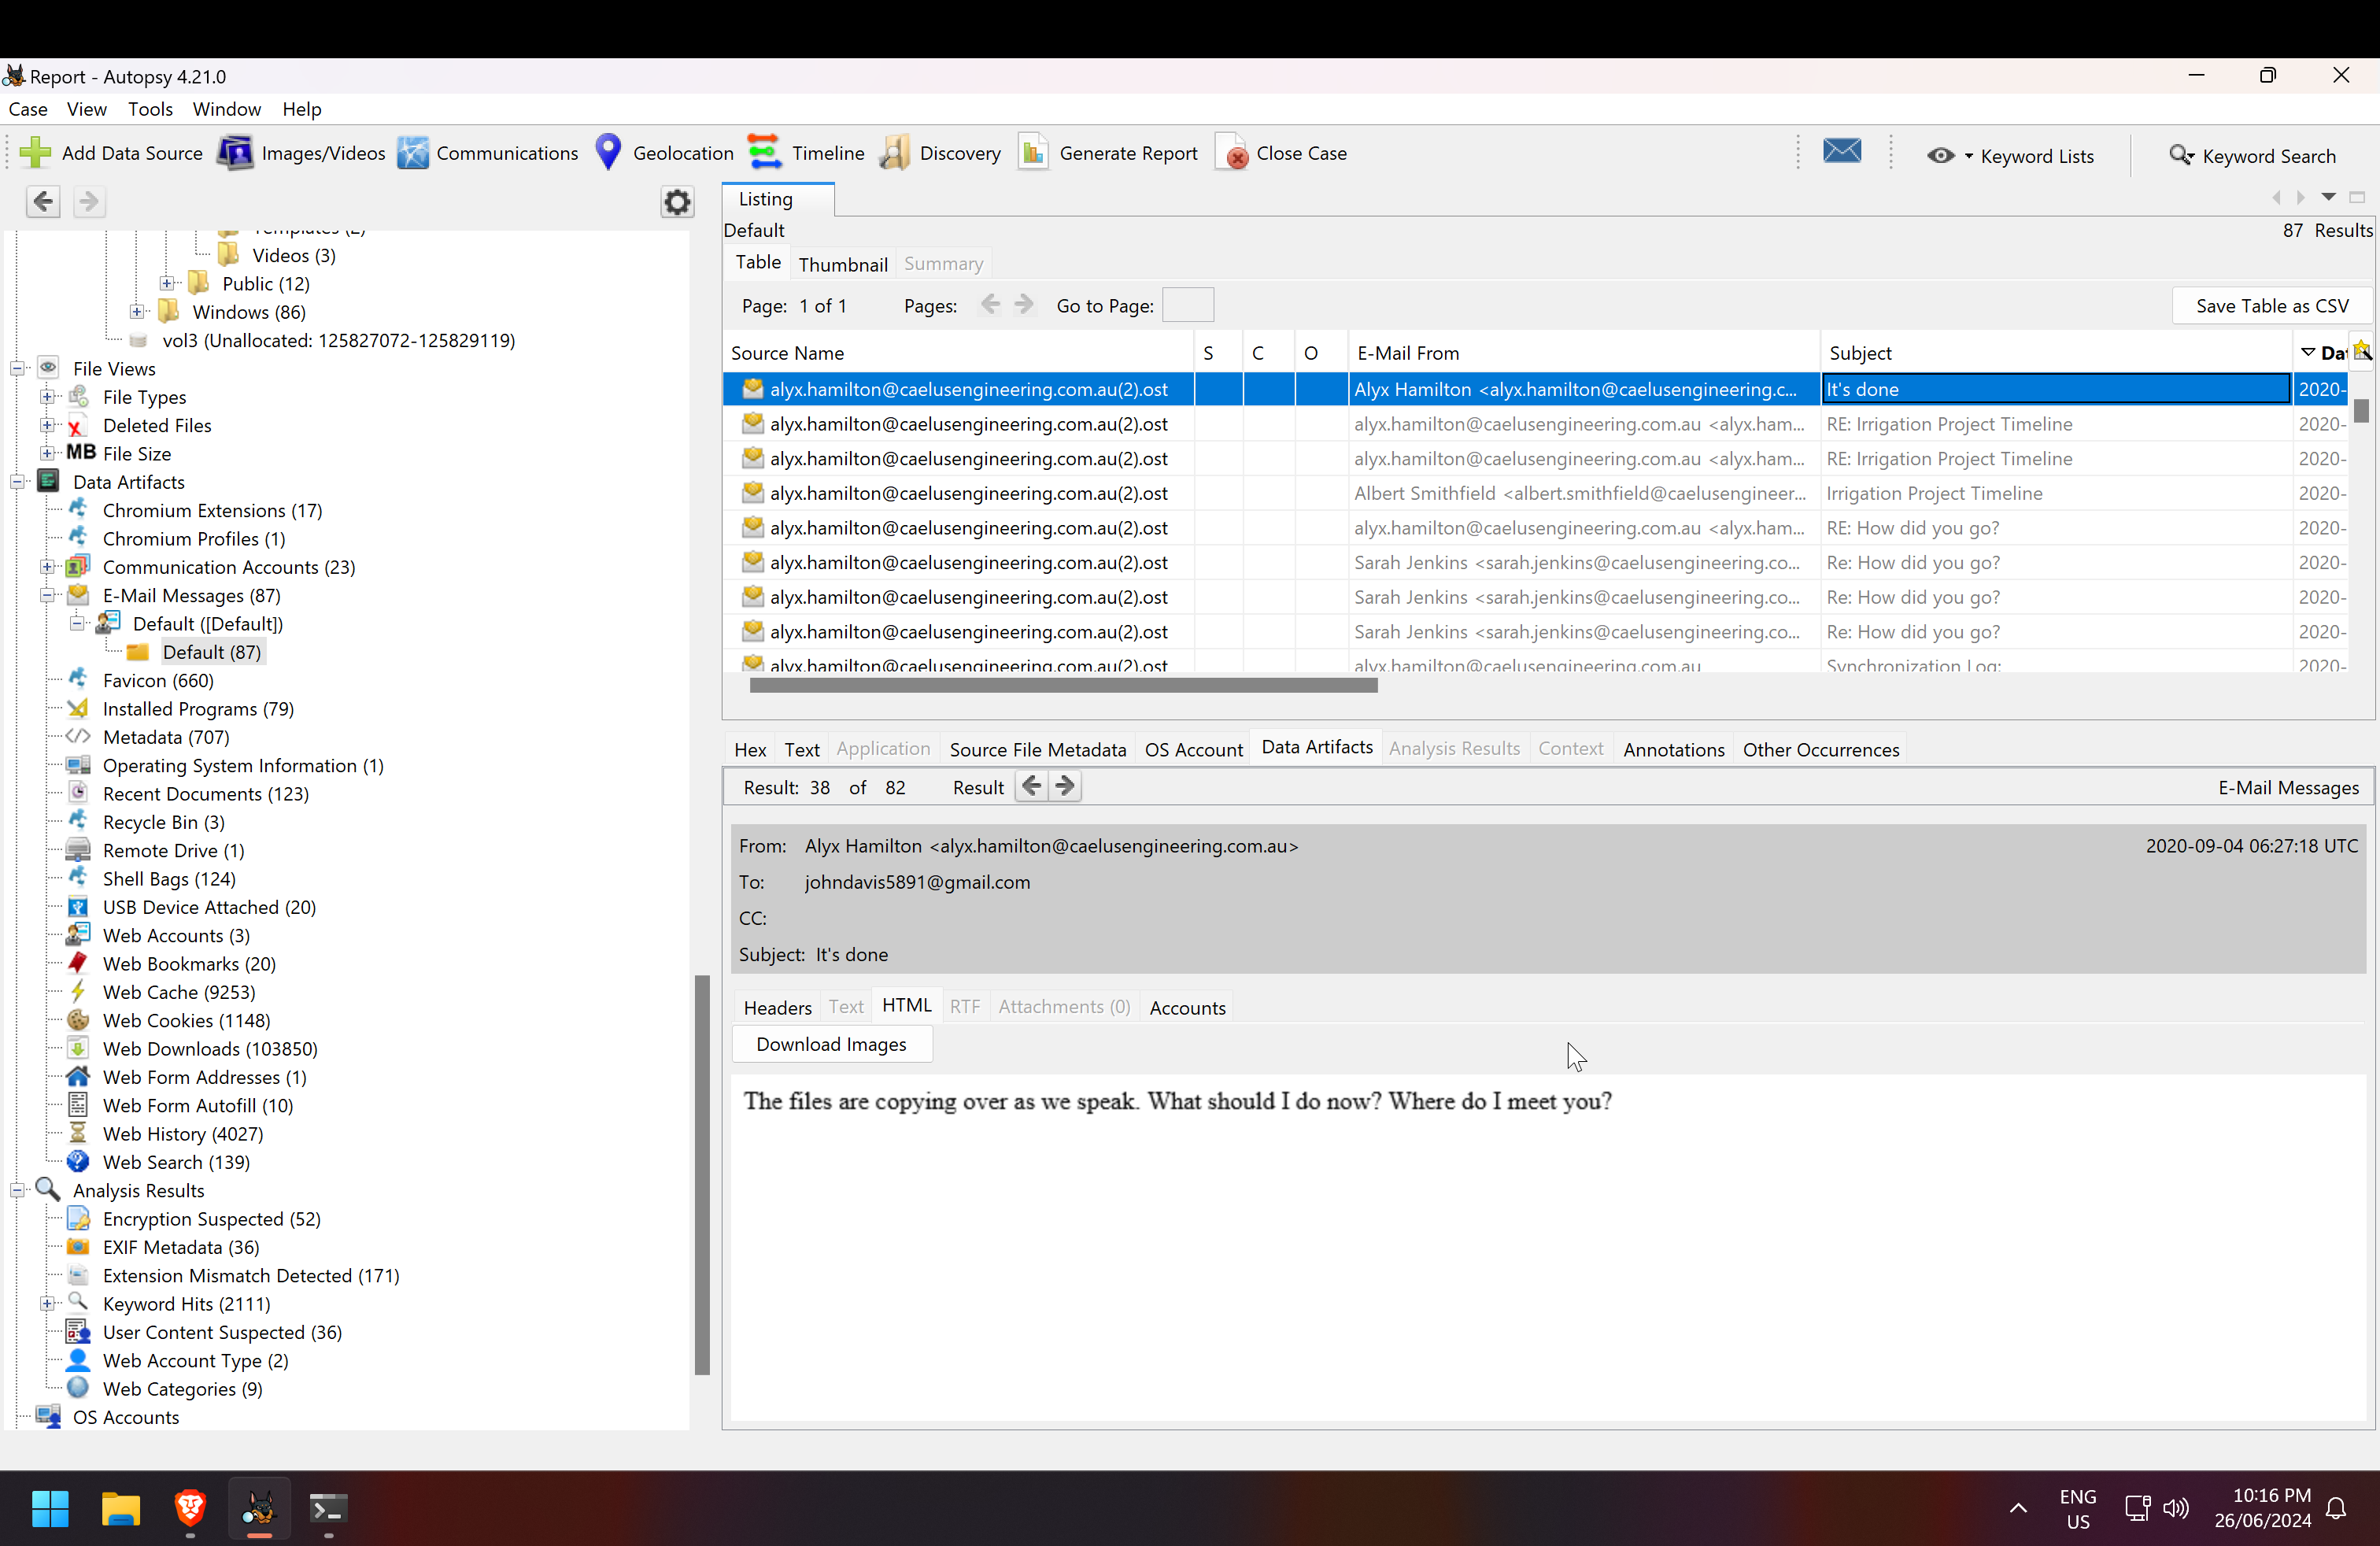
\includegraphics[width=1.0\textwidth]{email.png}
    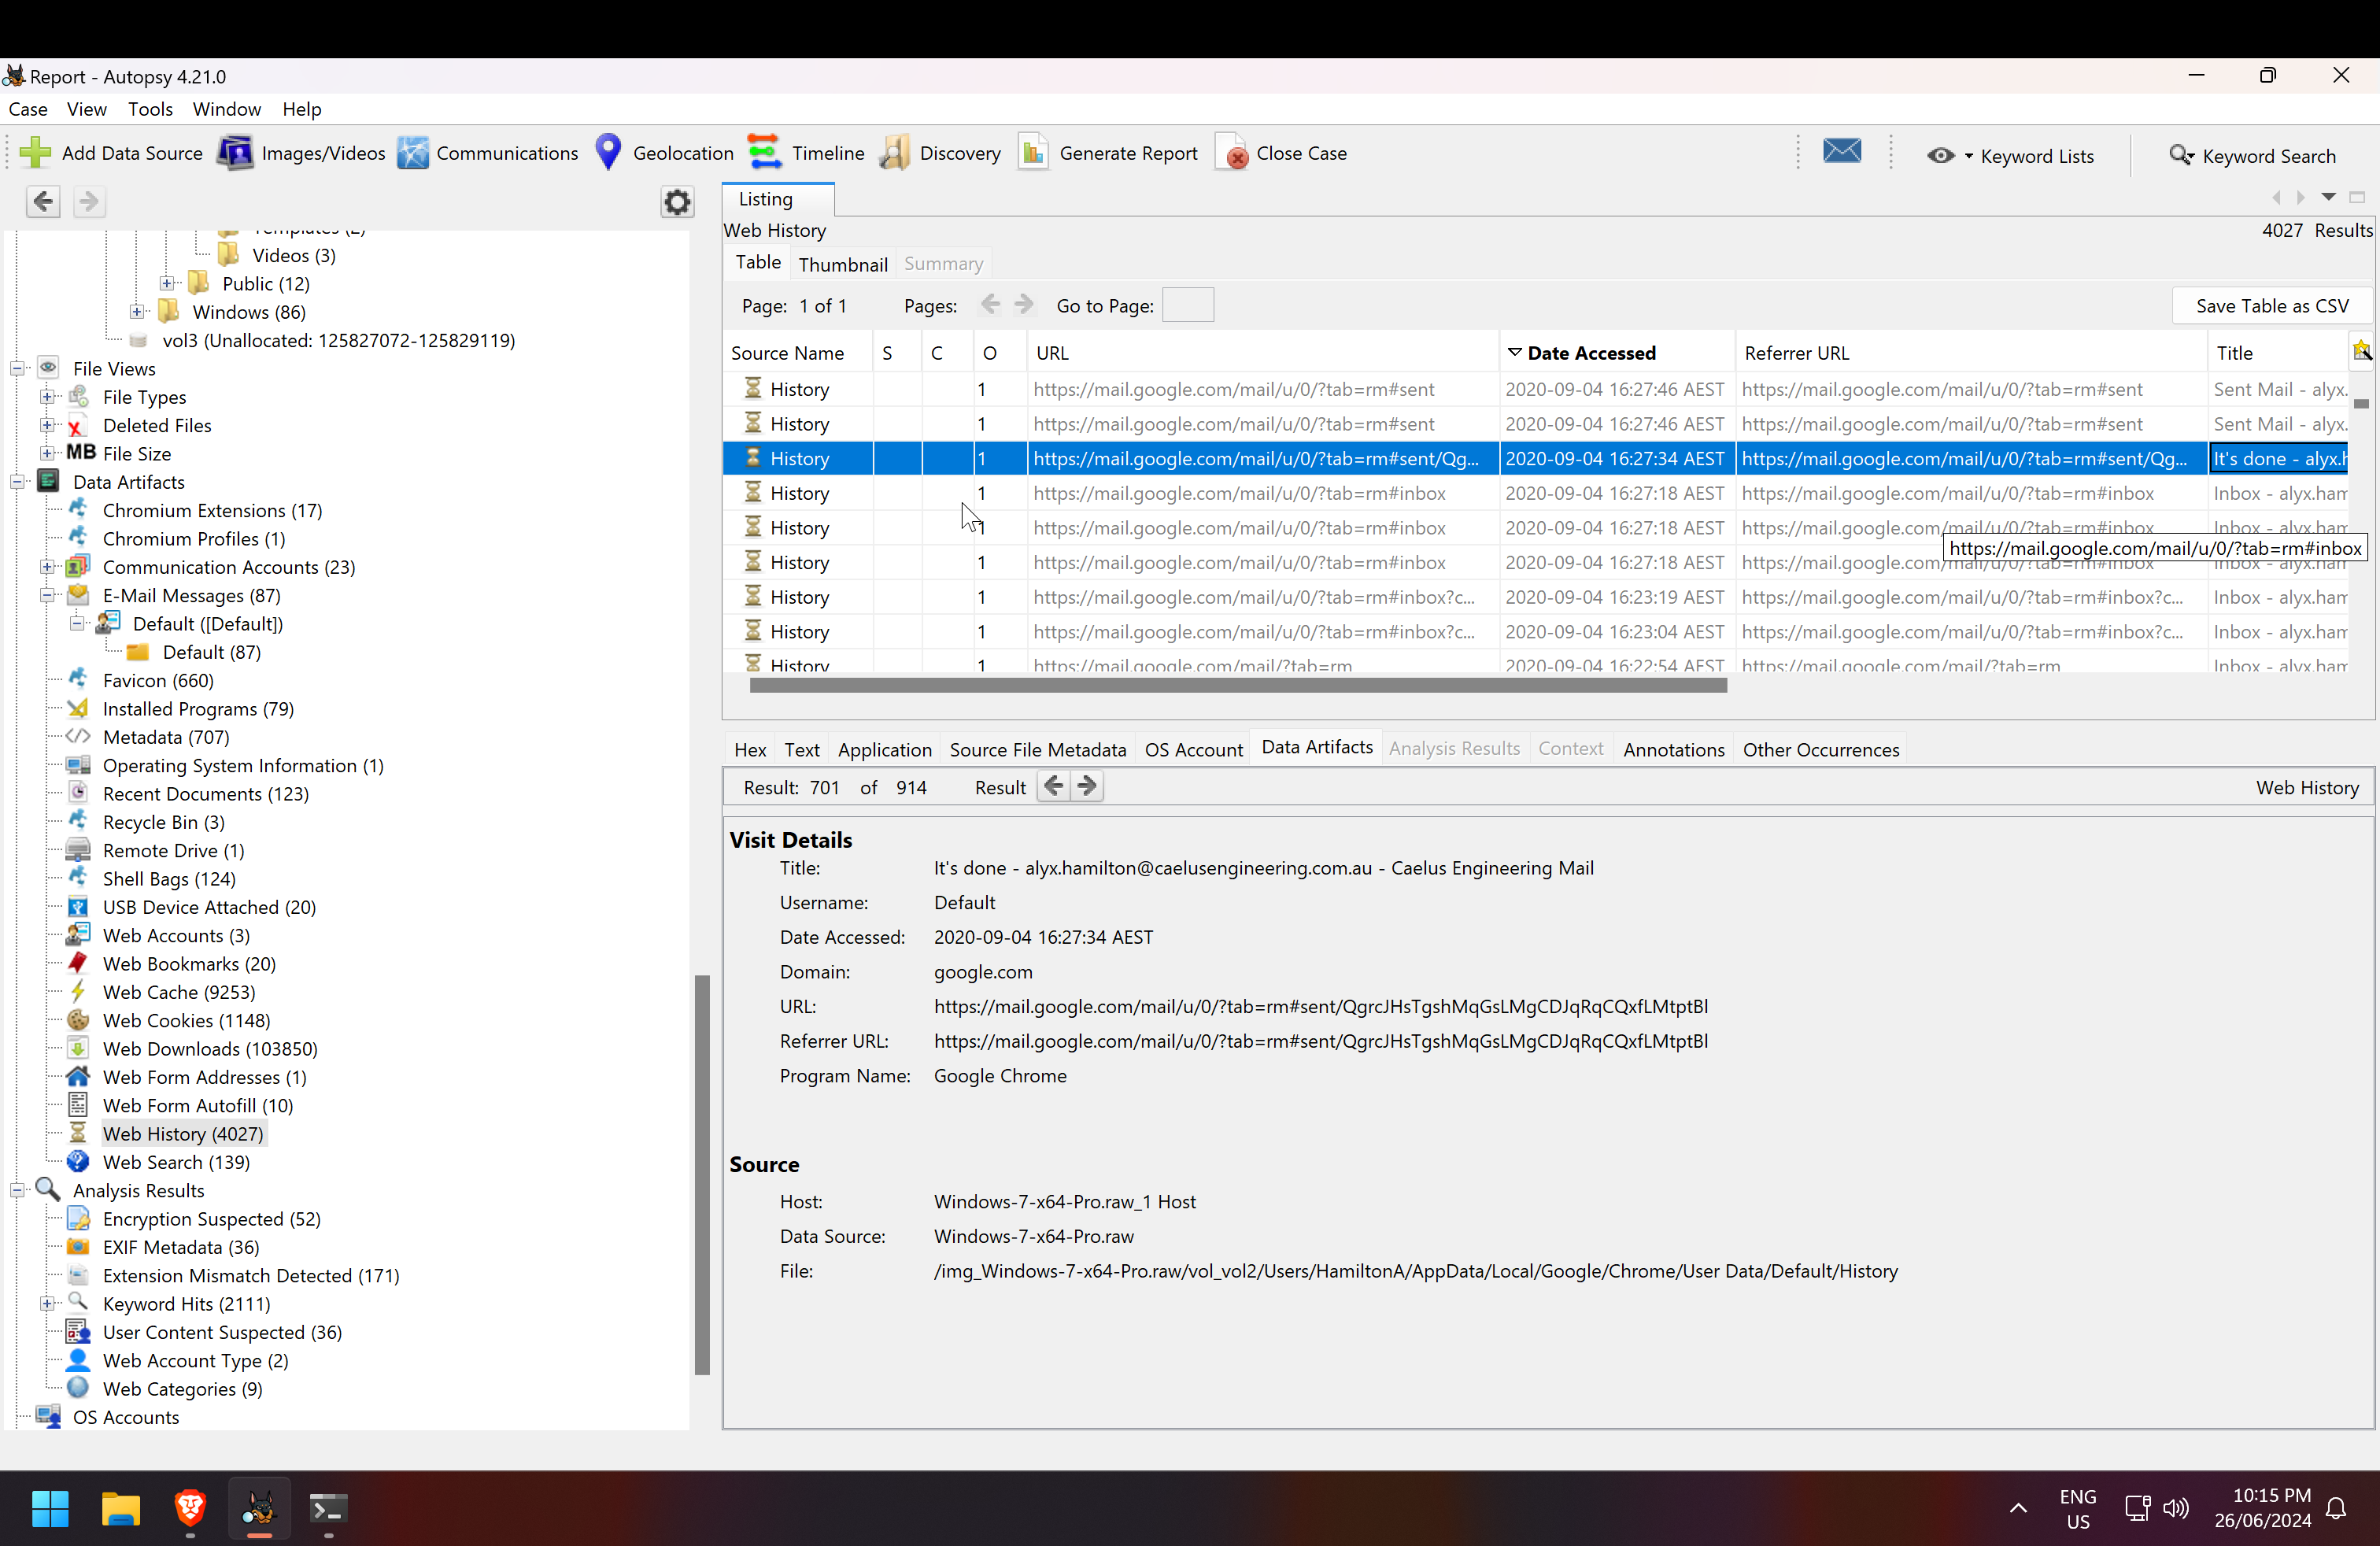
\includegraphics[width=1.0\textwidth]{email_browse_history.png}
    \caption{Cryptic email}
    \label{fig:email}
\end{figure}

\begin{figure}[H]
    \centering
    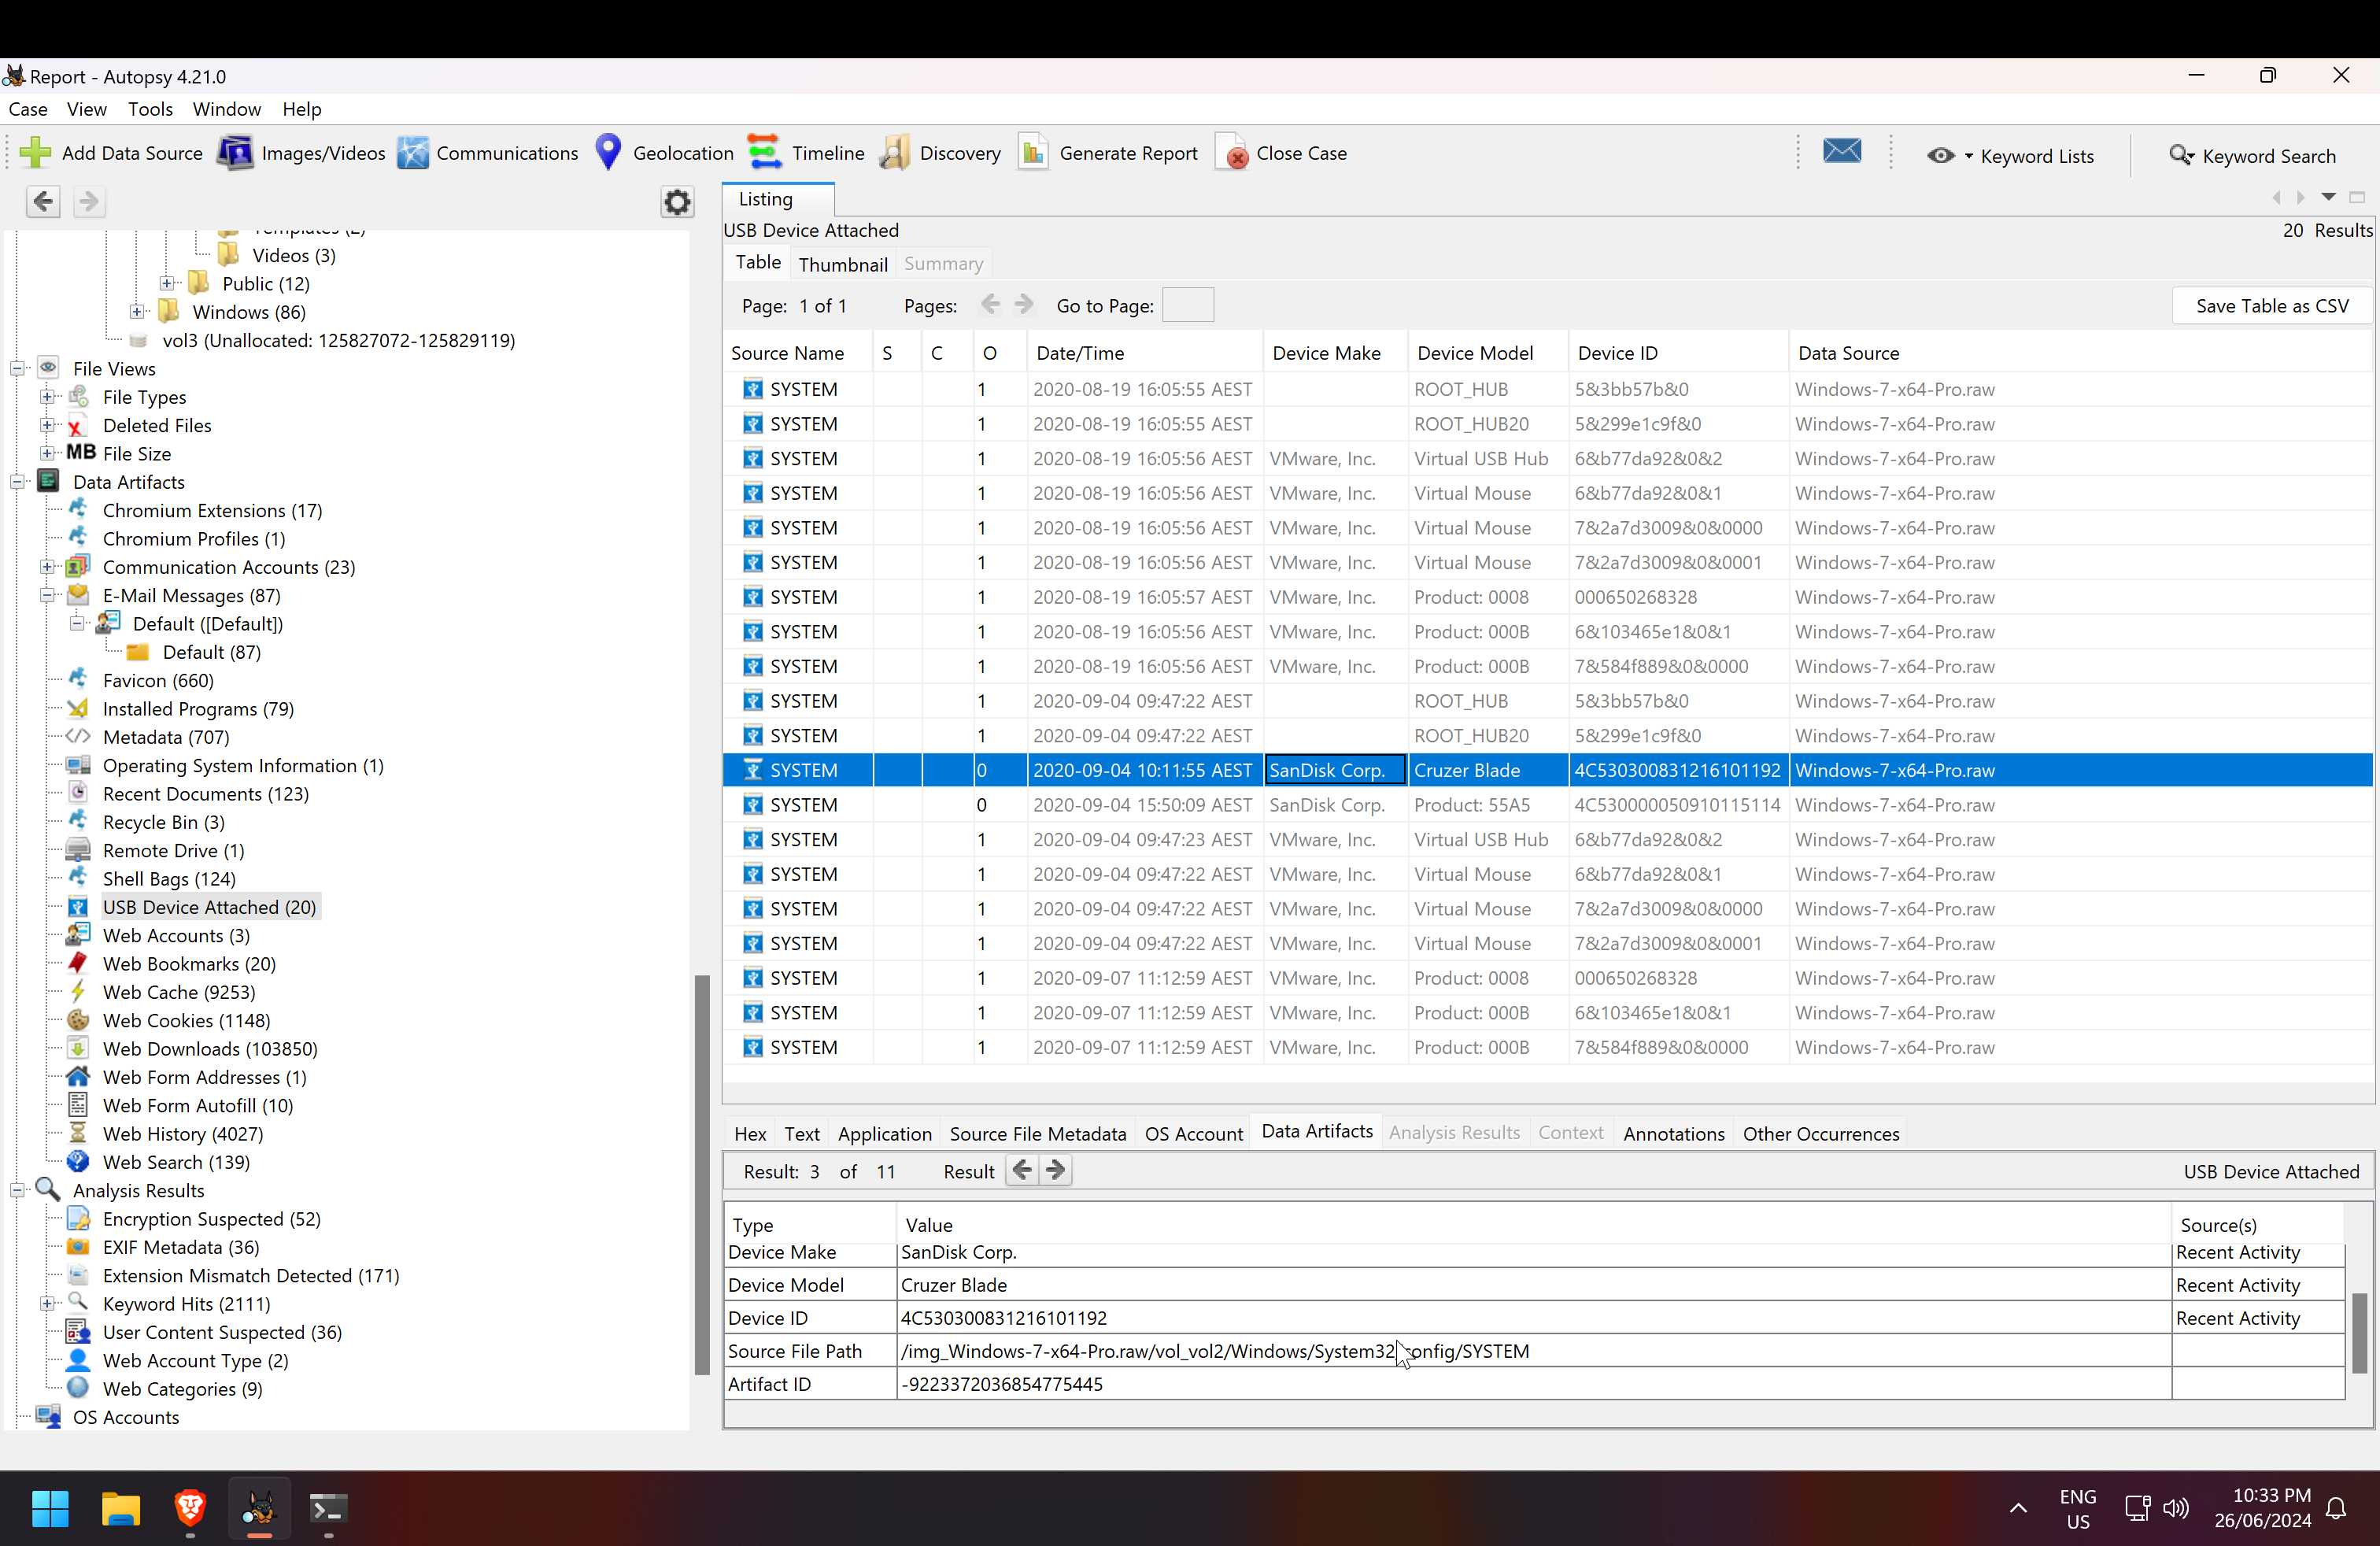
\includegraphics[width=1.0\textwidth]{usb1.png}
    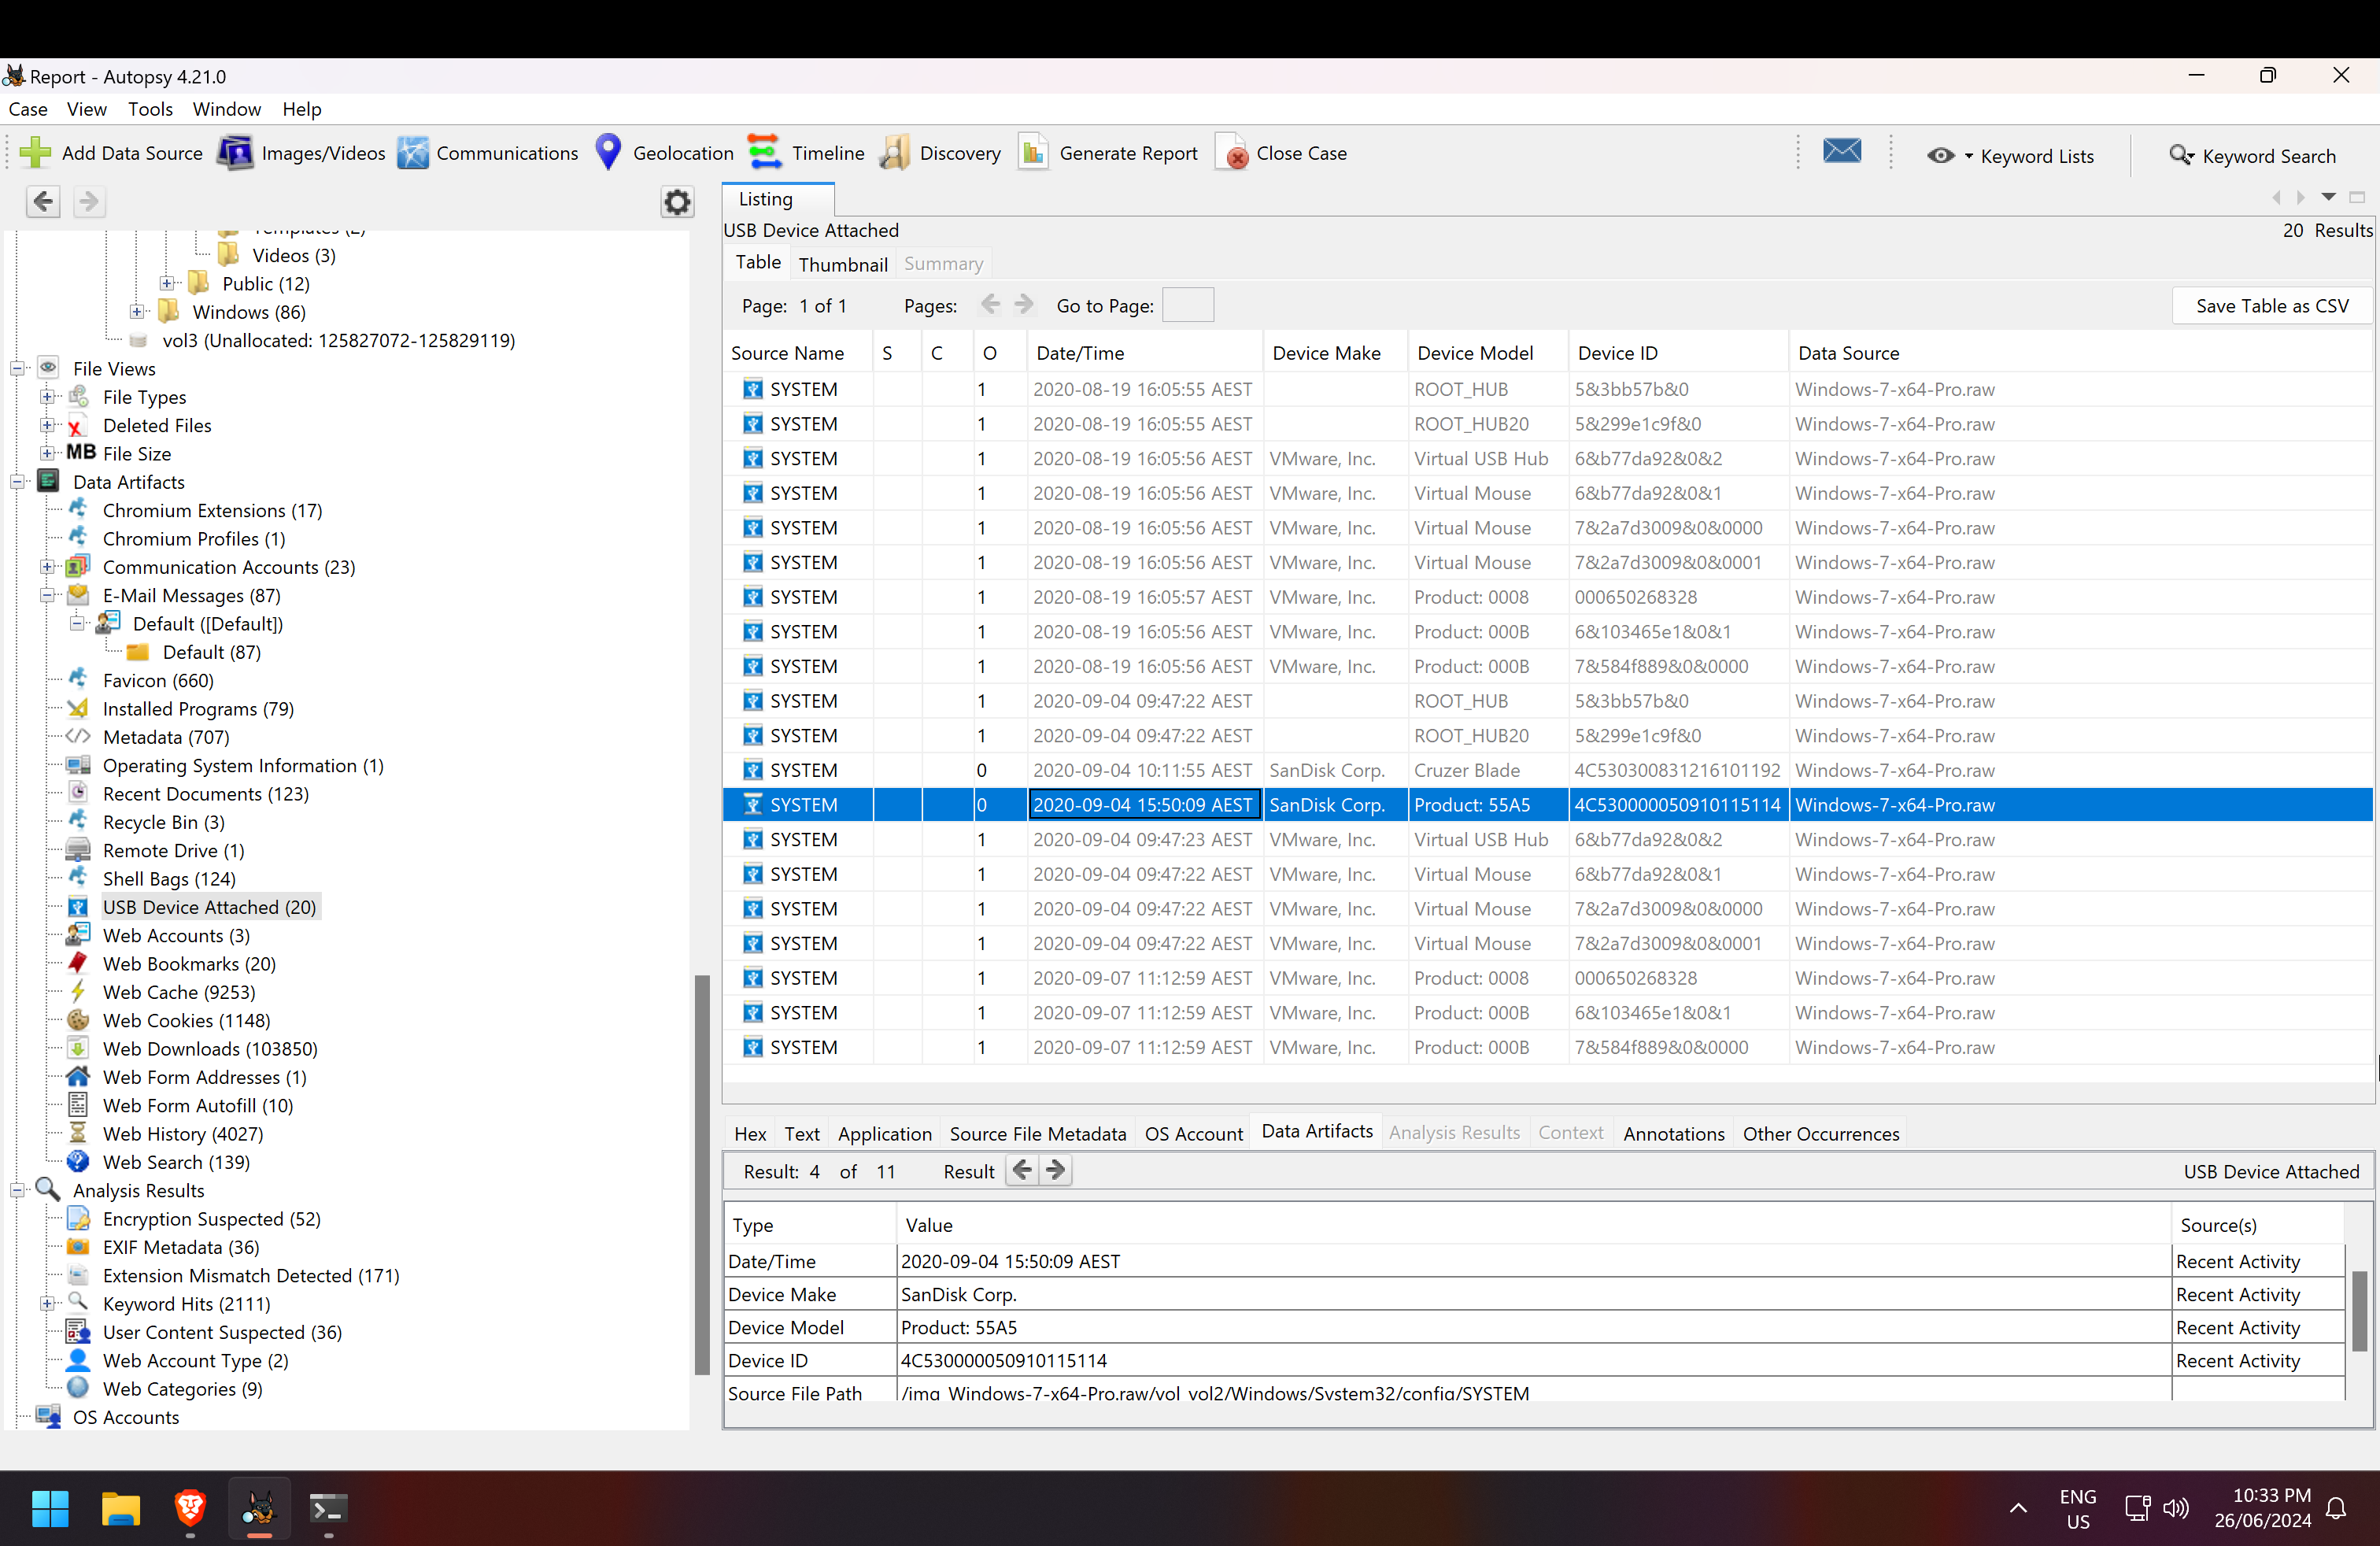
\includegraphics[width=1.0\textwidth]{usb2.png}
    \caption{Attached USB drives}
    \label{fig:usb}
\end{figure}

\begin{figure}[H]
    \centering
    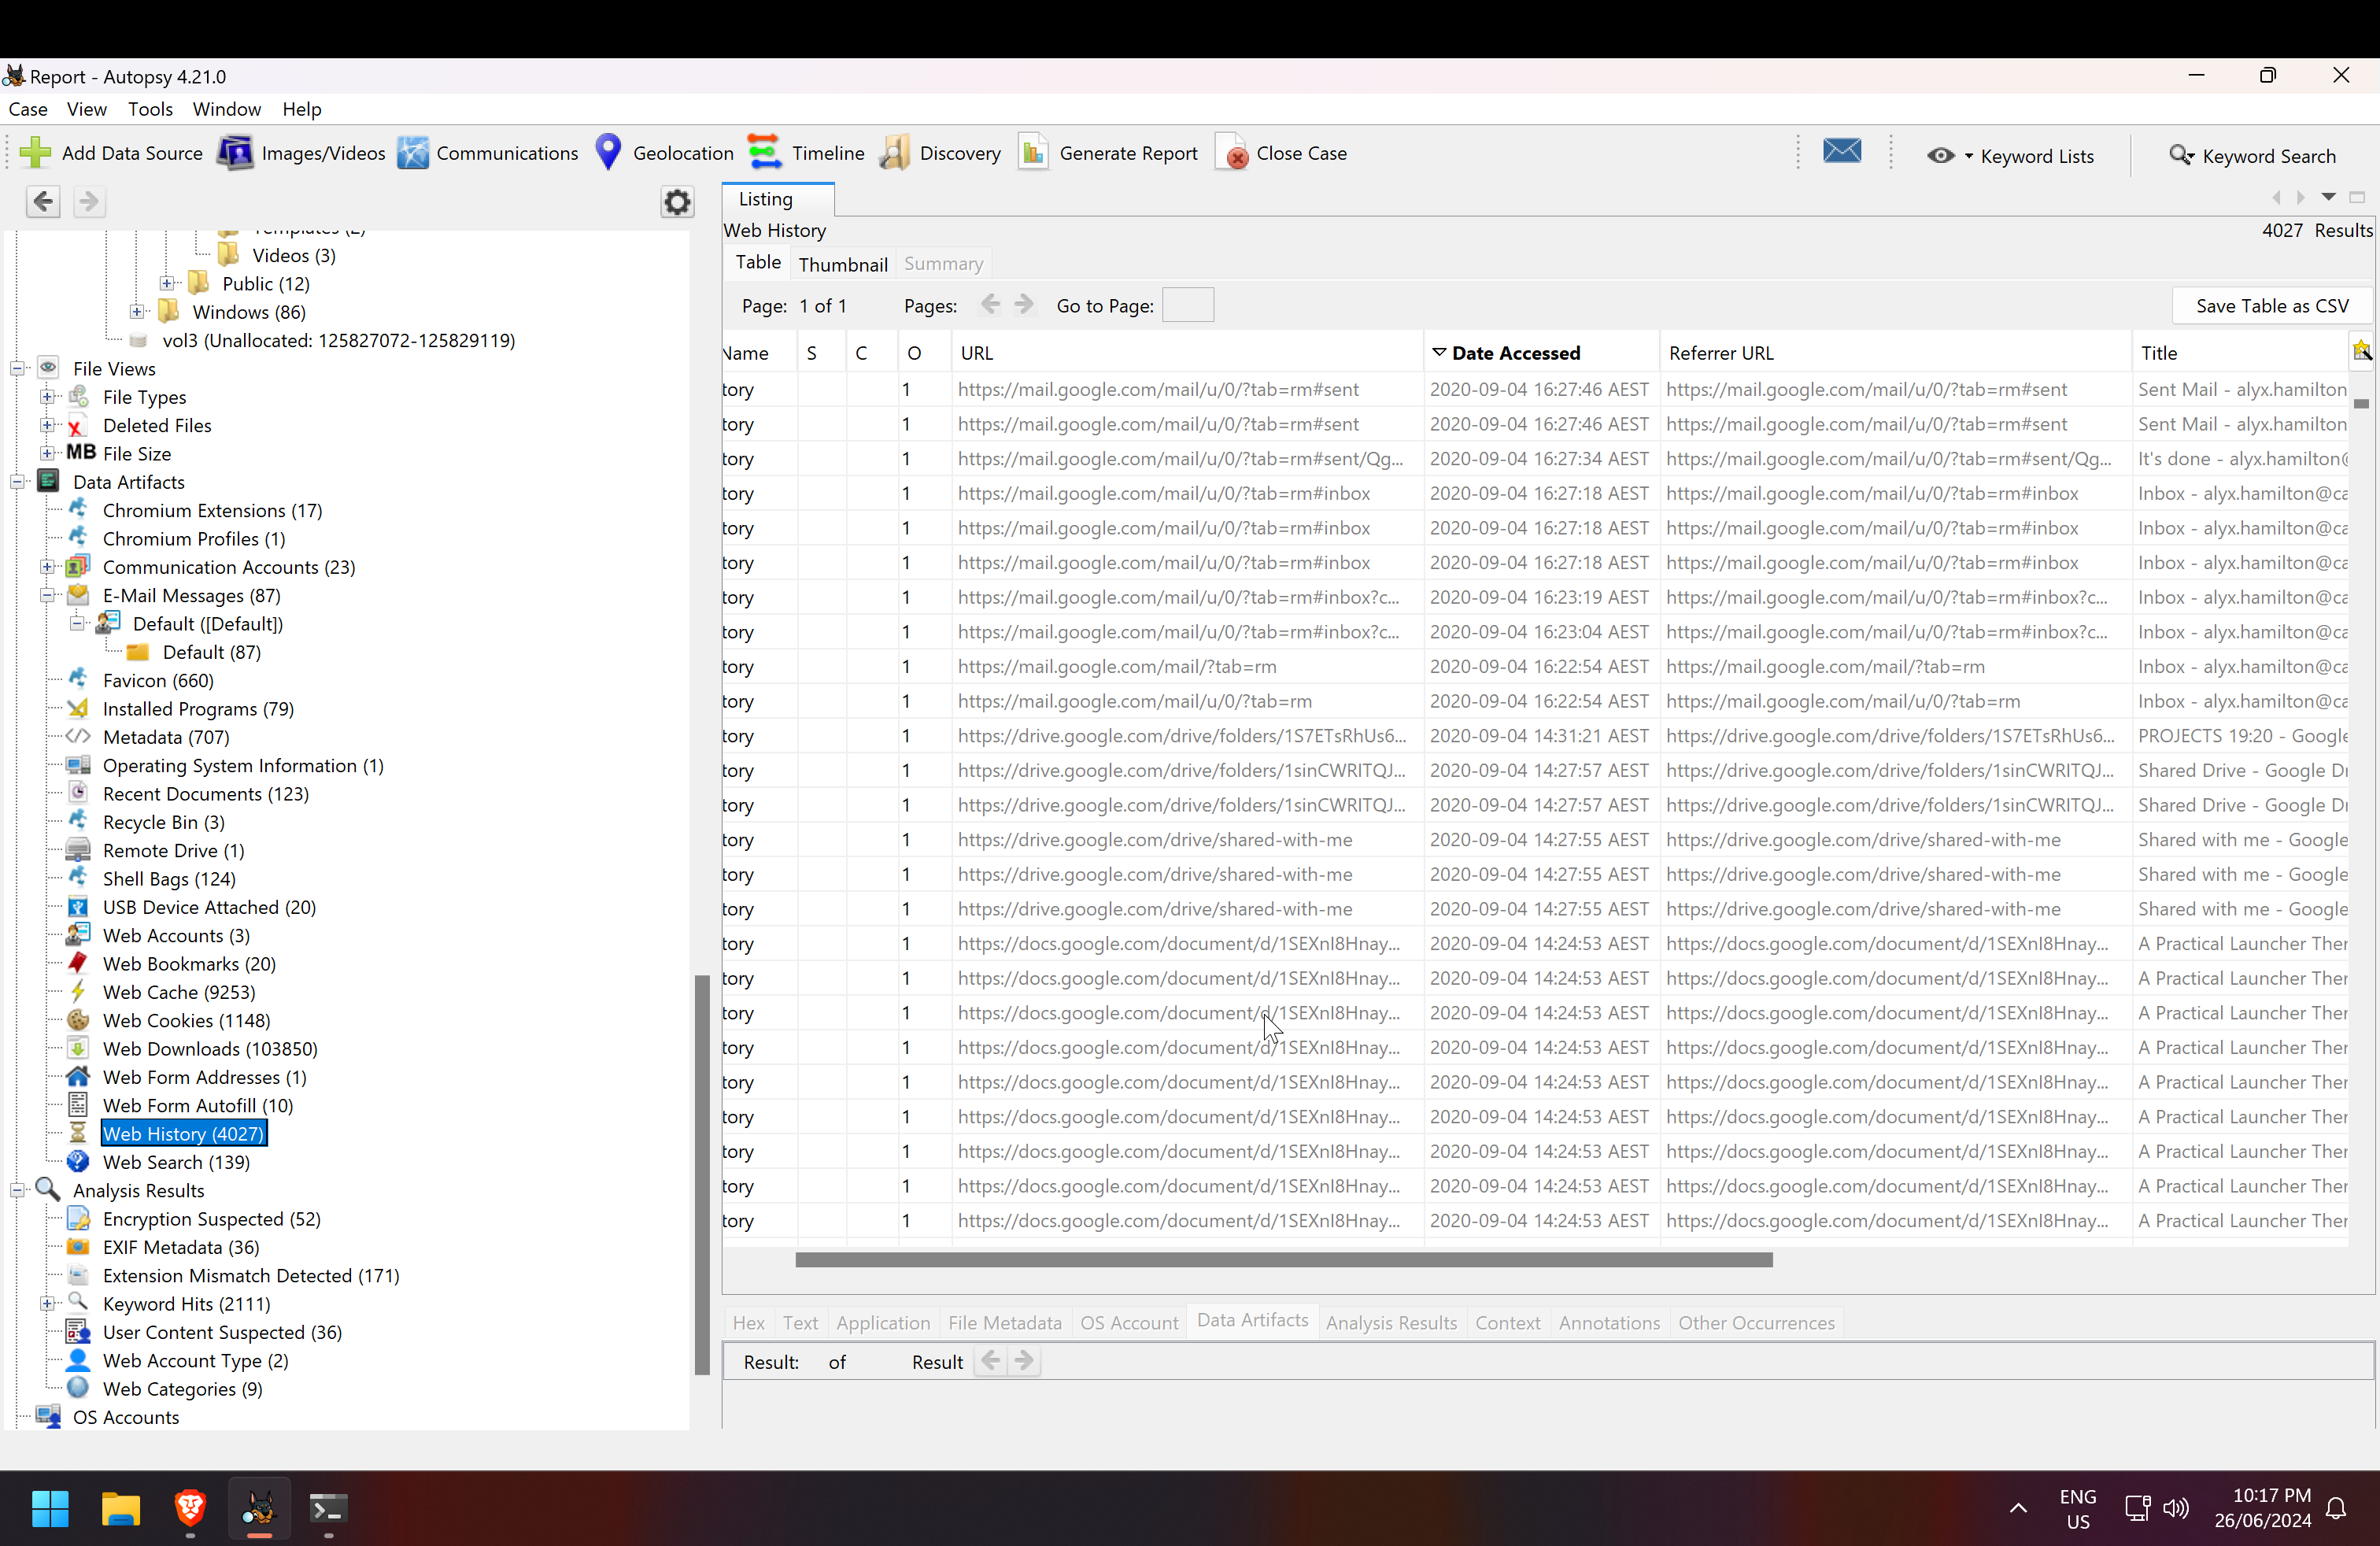
\includegraphics[width=1.0\textwidth]{history1.png}
    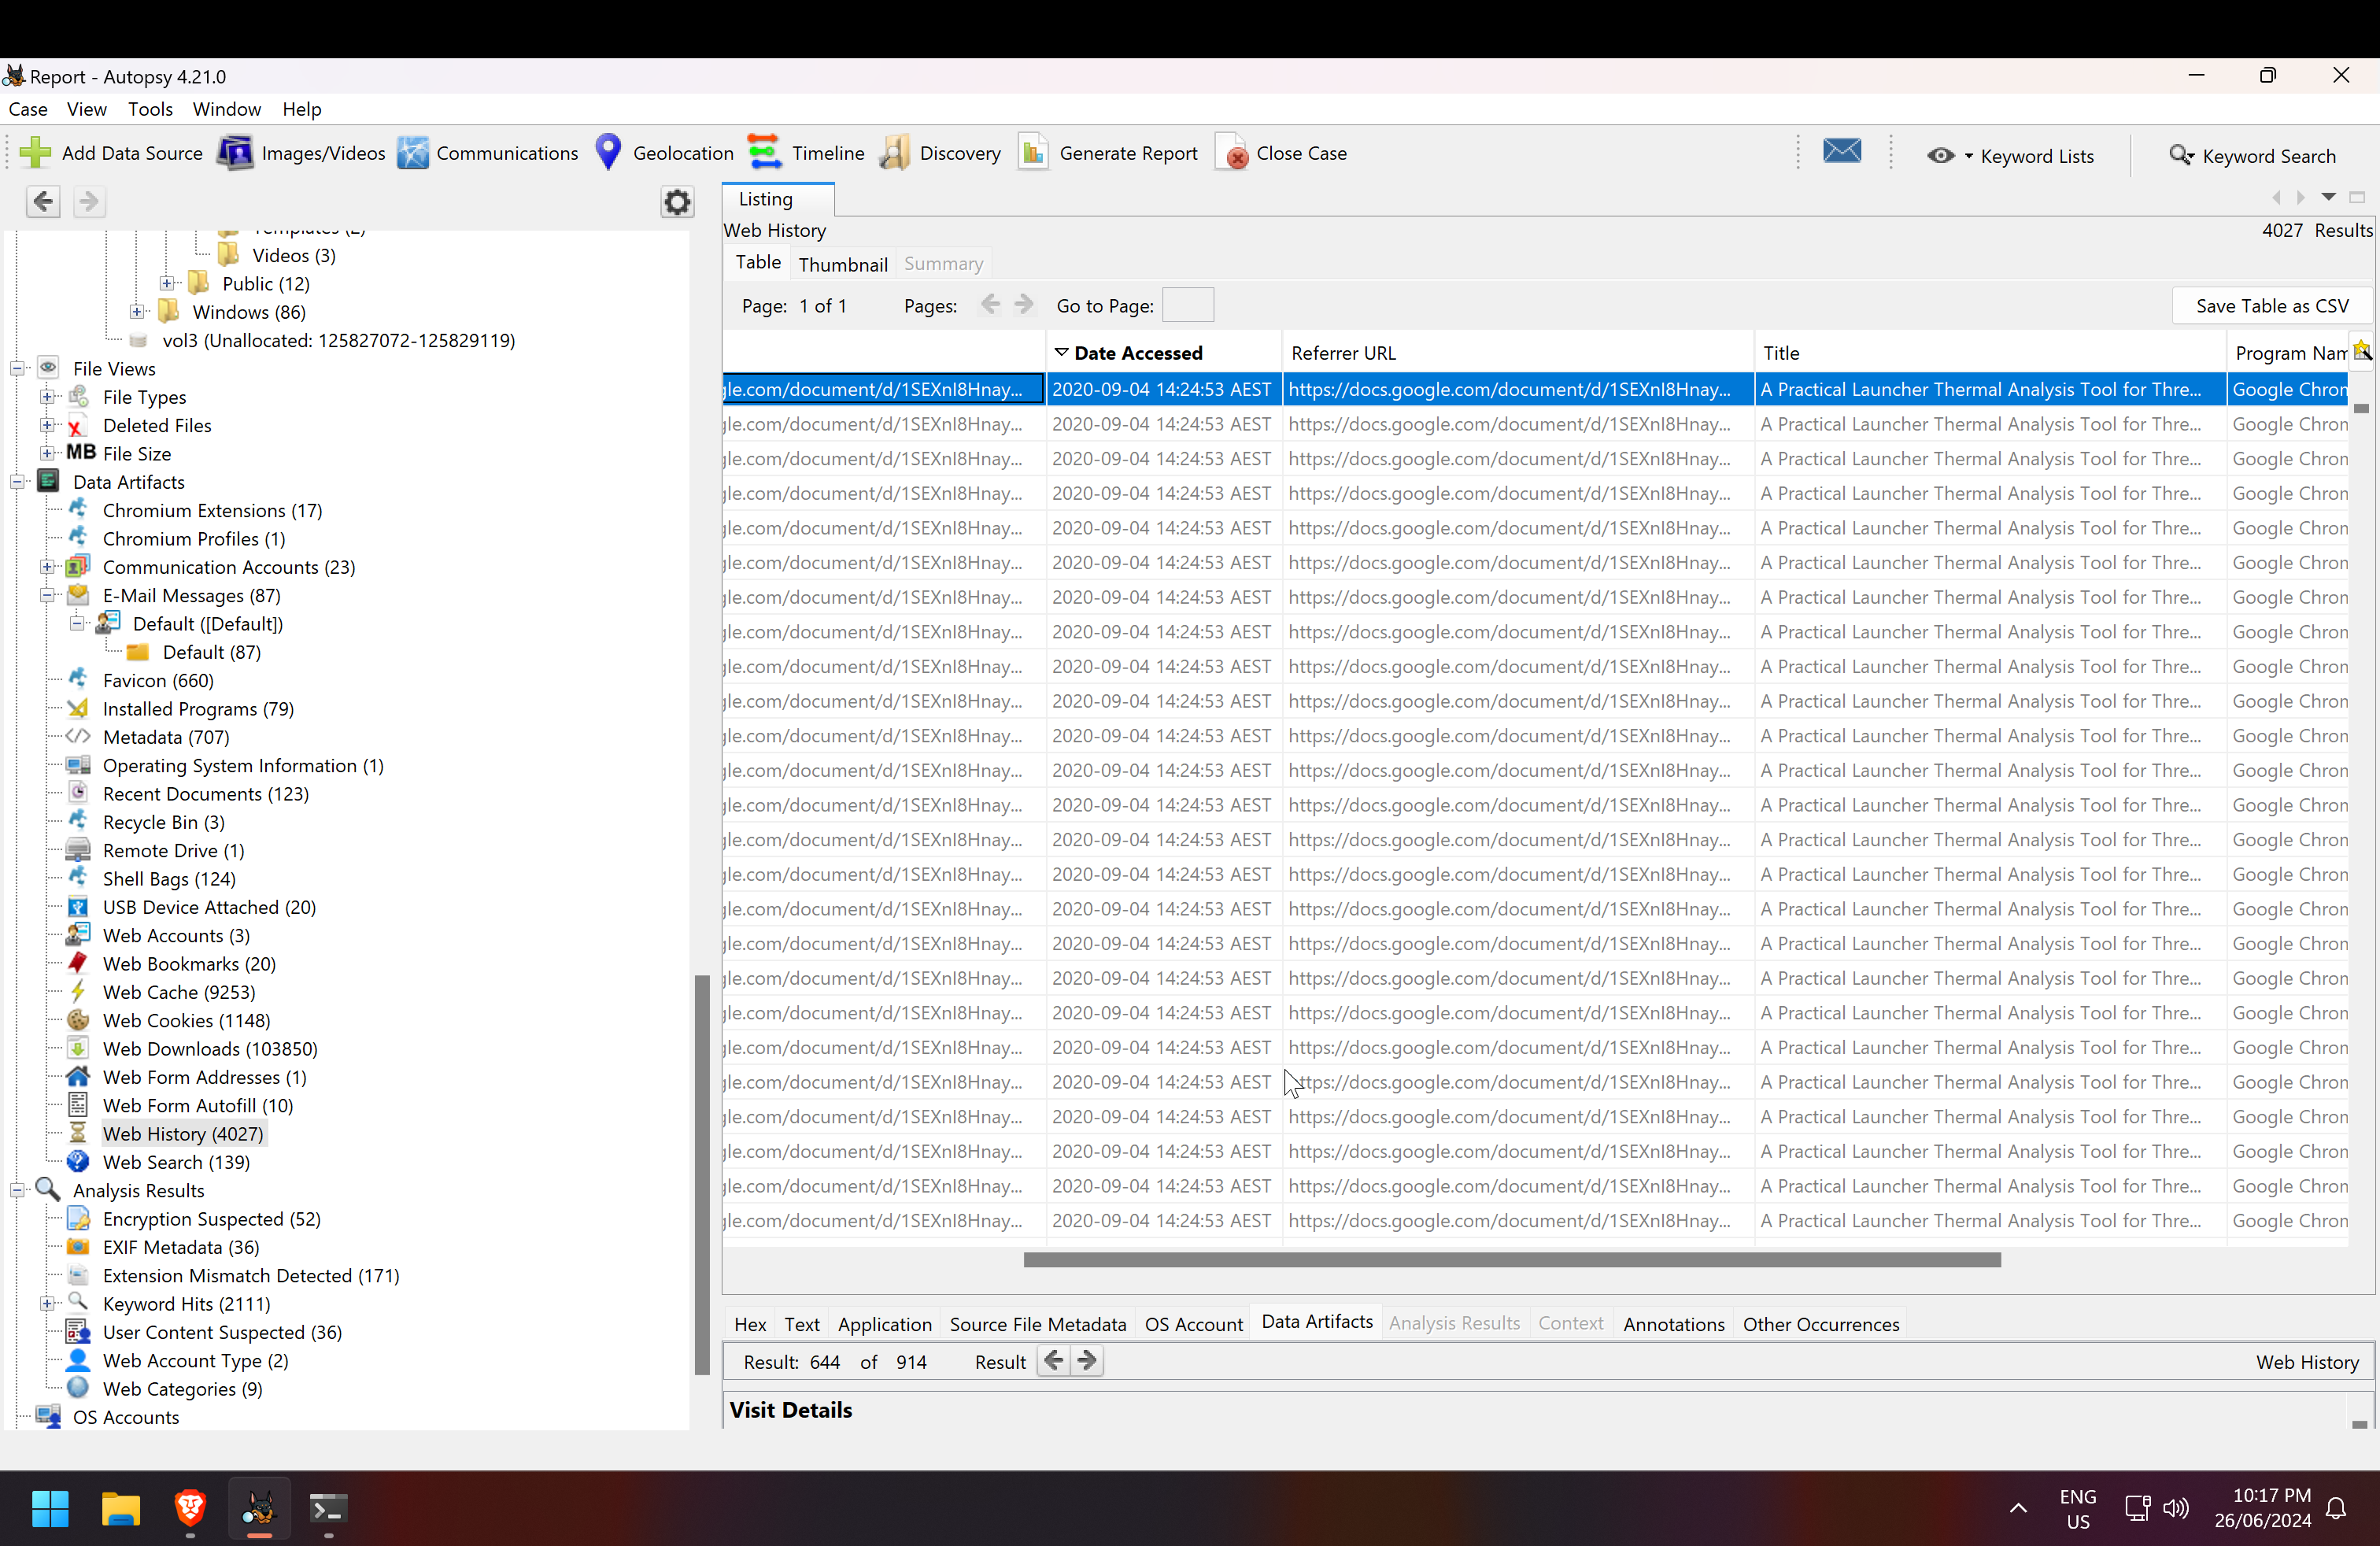
\includegraphics[width=1.0\textwidth]{history2.png}
    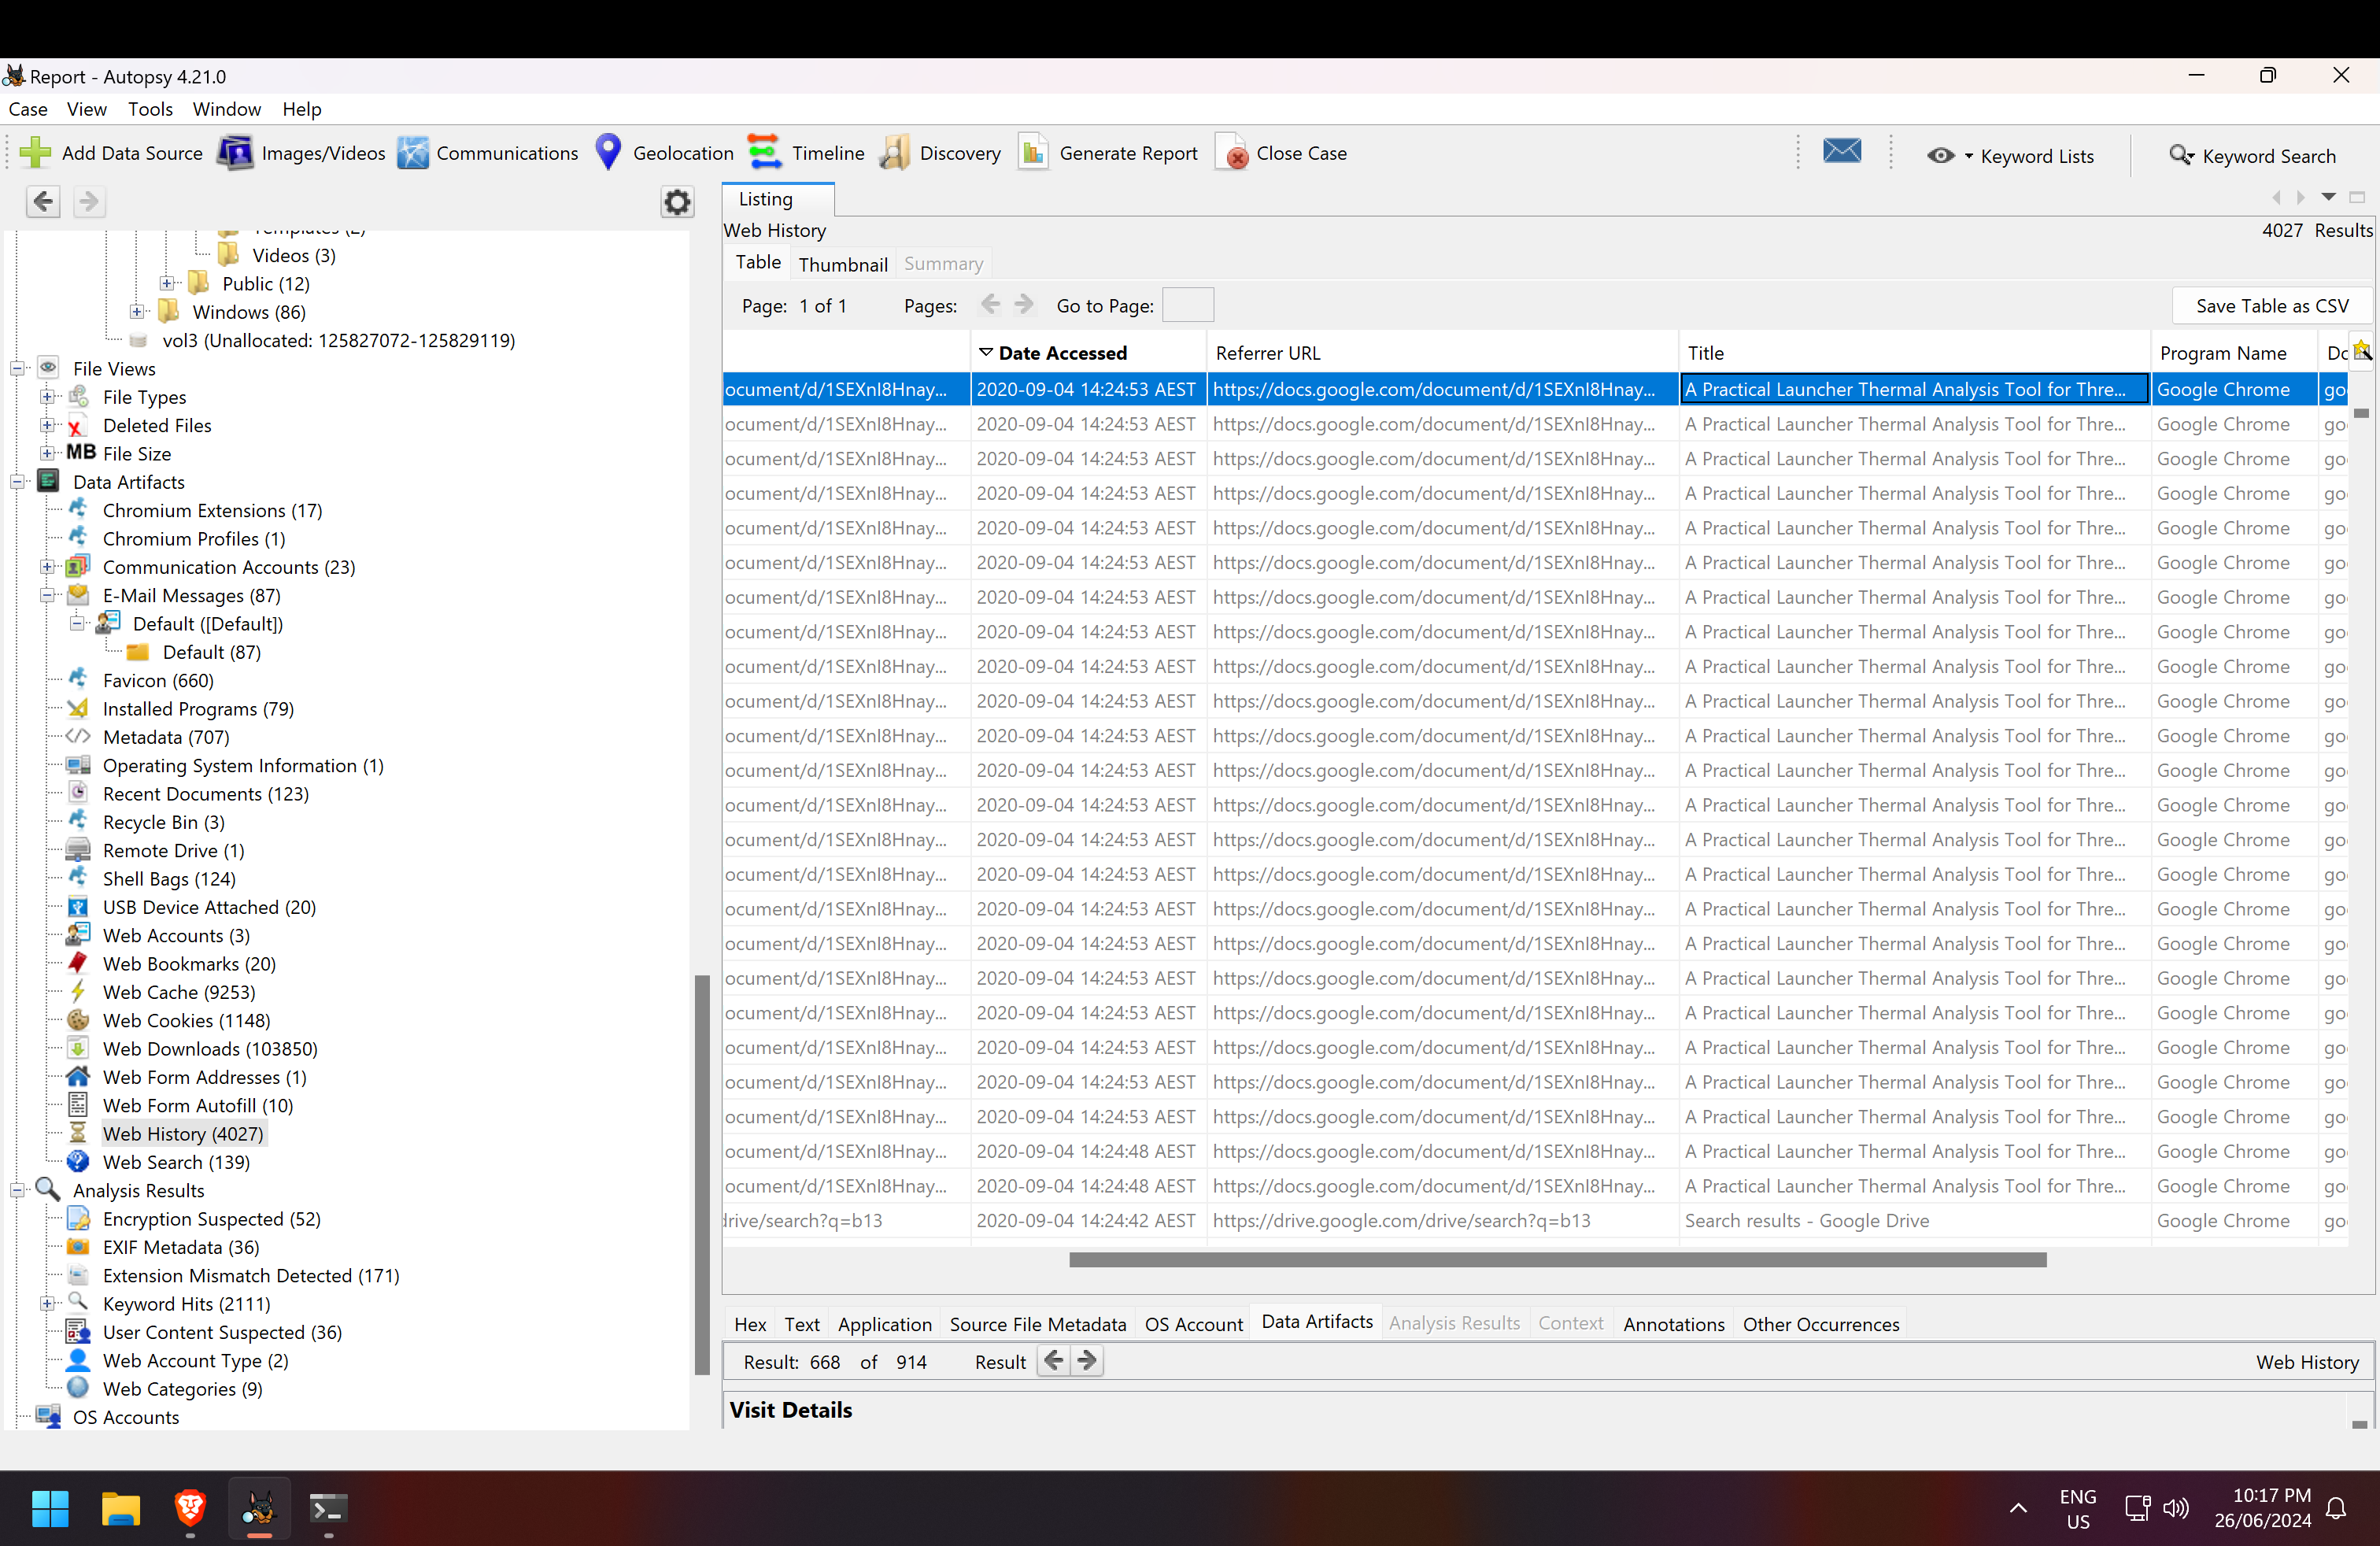
\includegraphics[width=1.0\textwidth]{history3.png}
    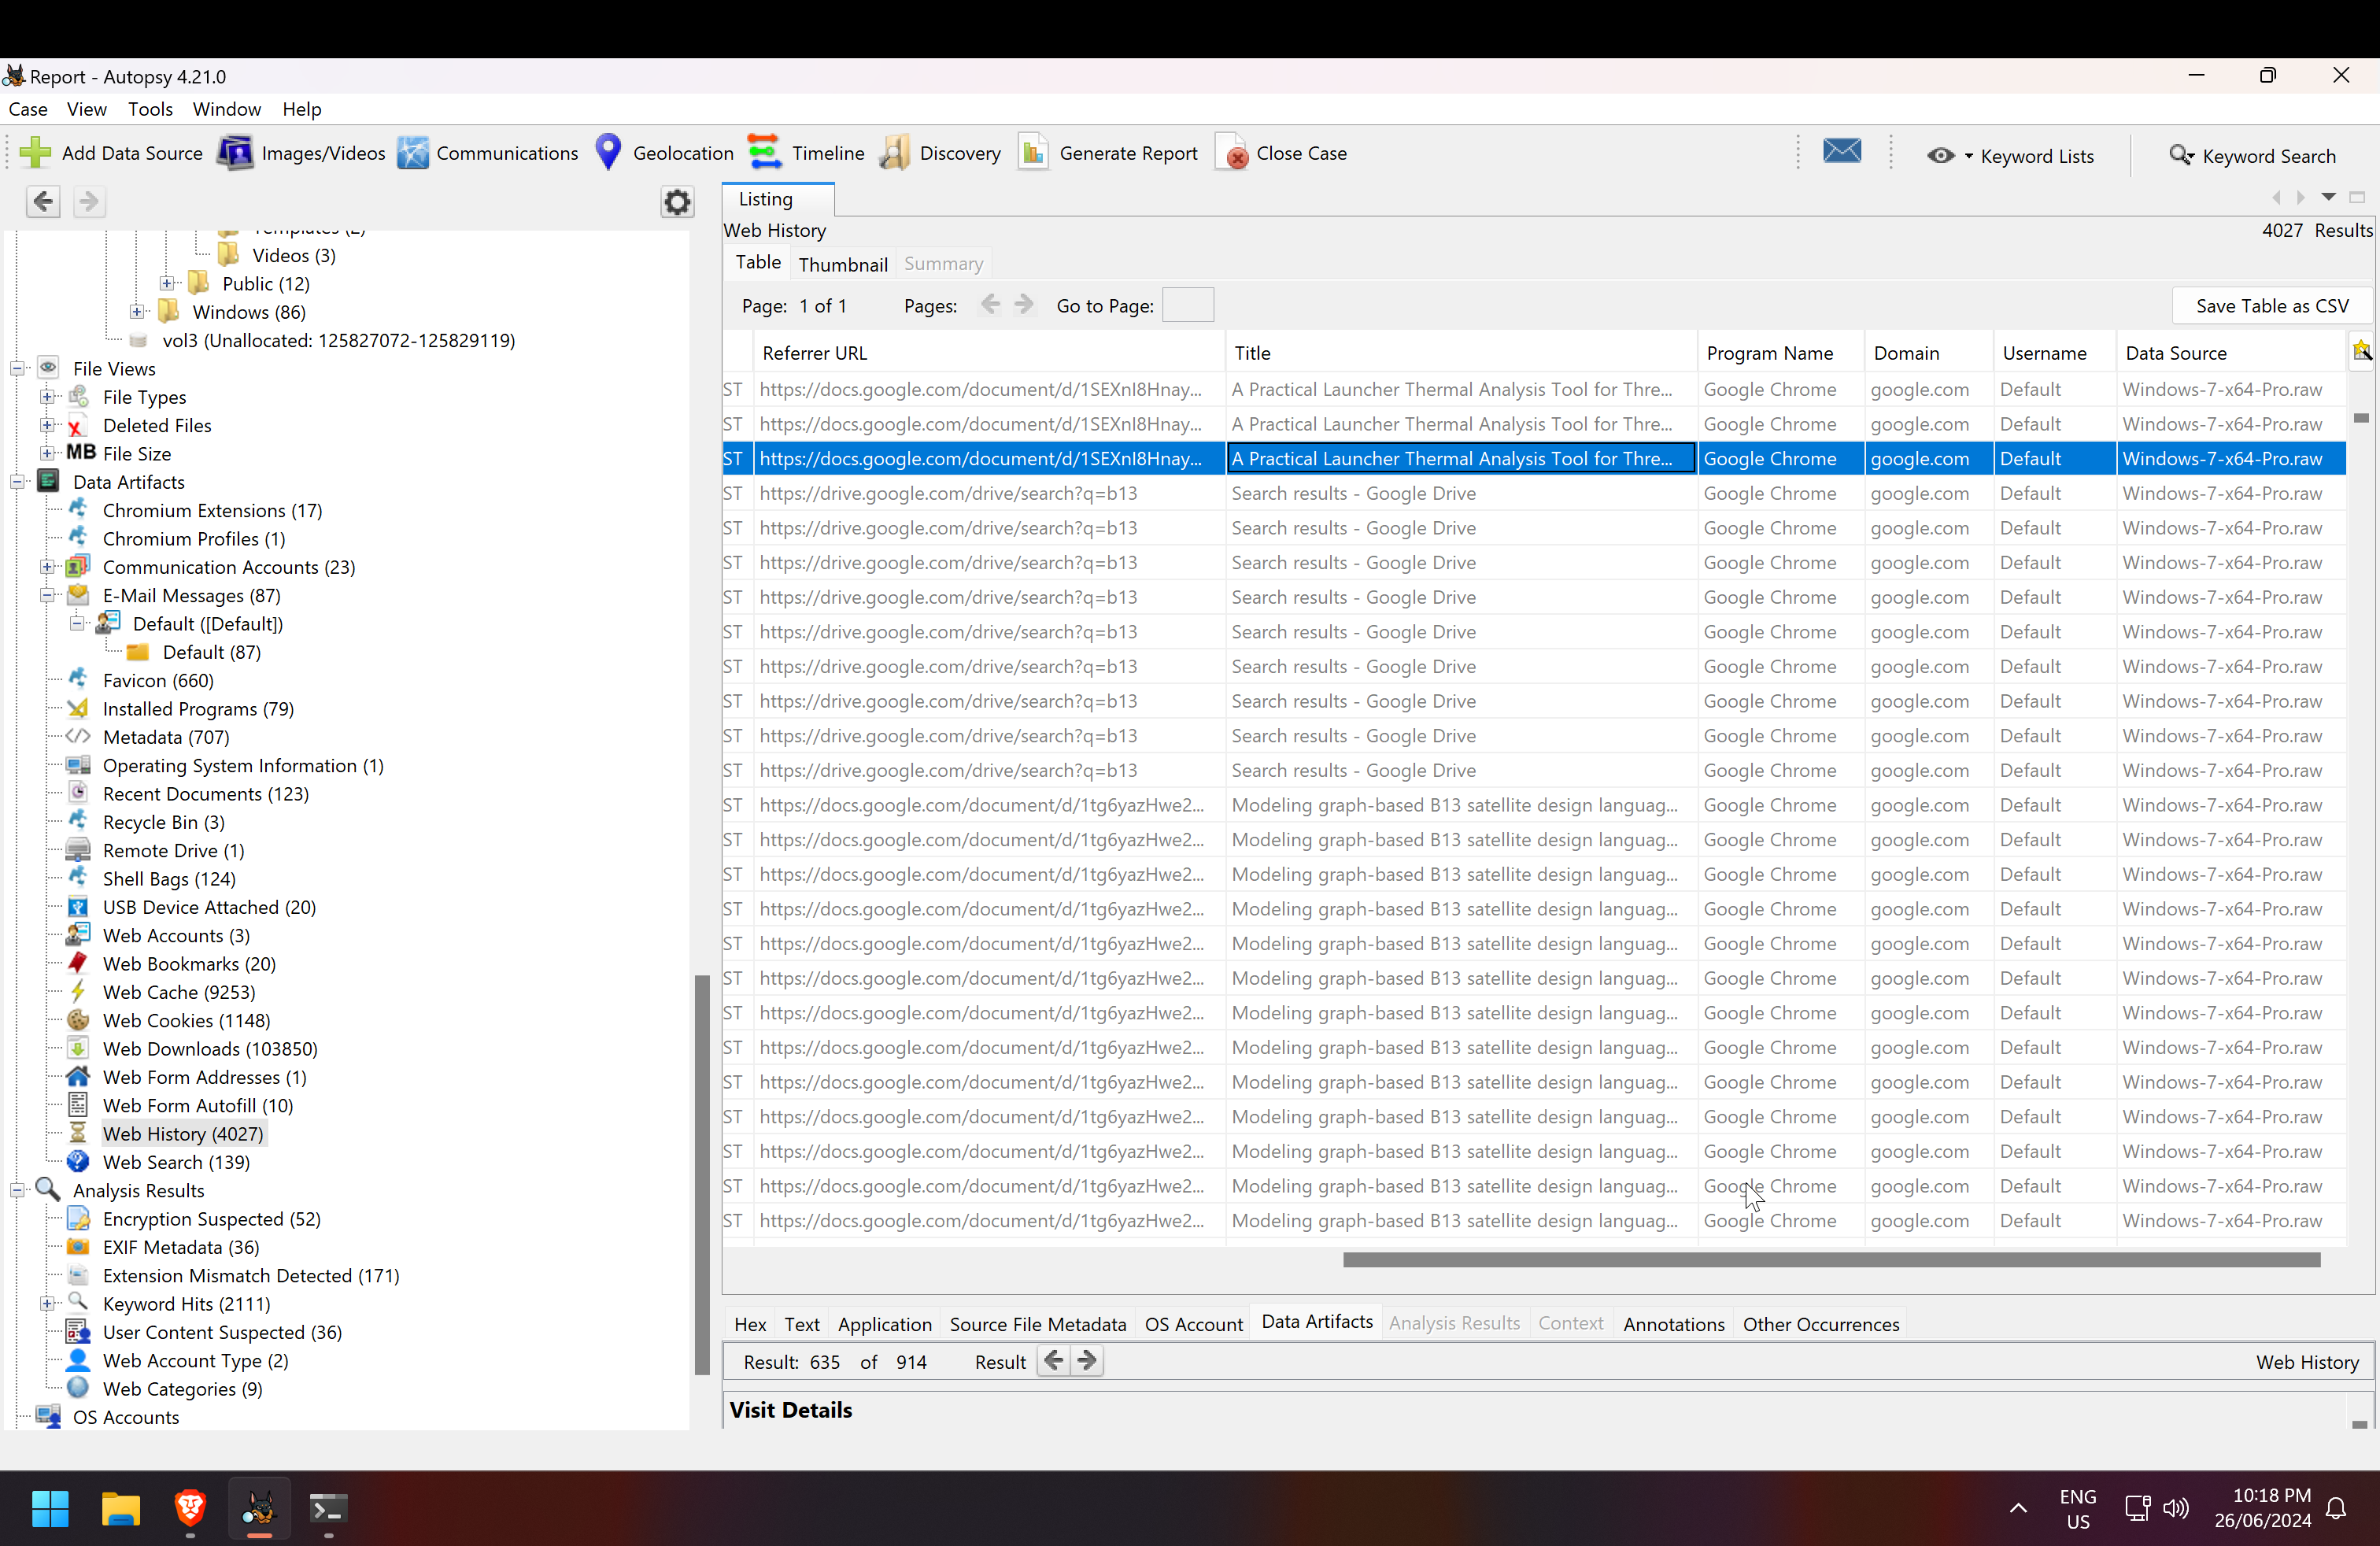
\includegraphics[width=1.0\textwidth]{history4.png}
    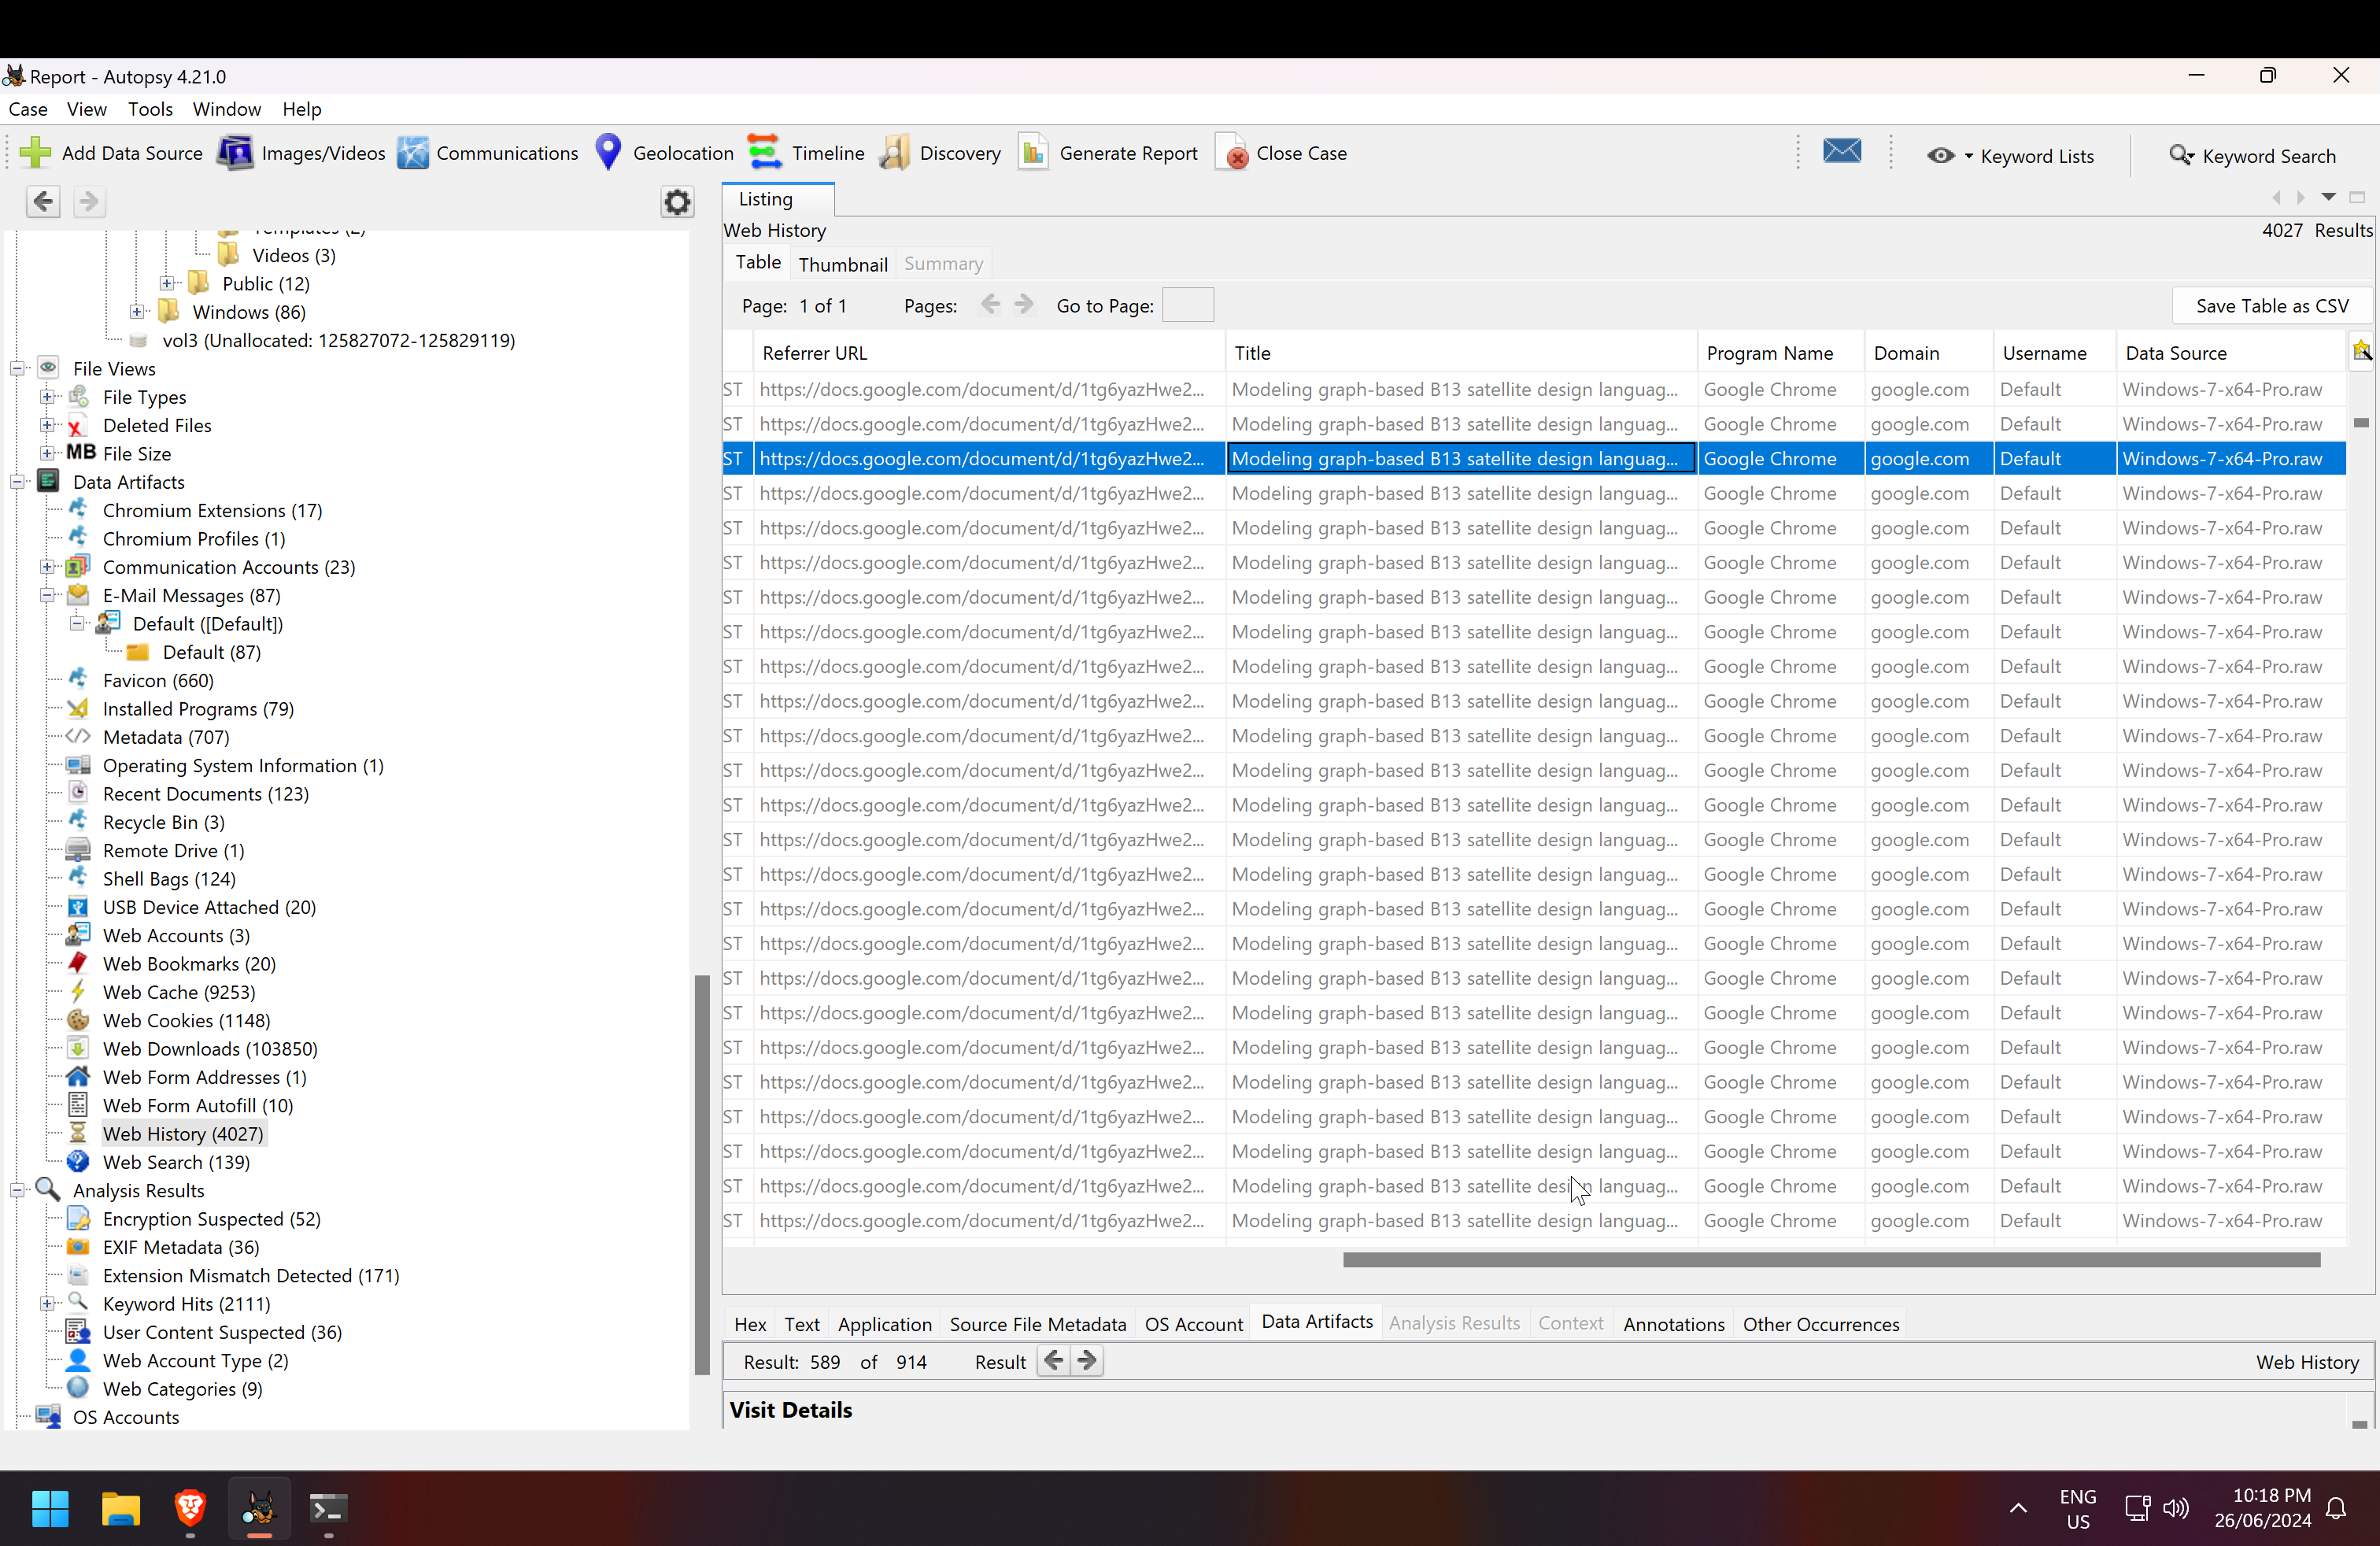
\includegraphics[width=1.0\textwidth]{history5.png}
    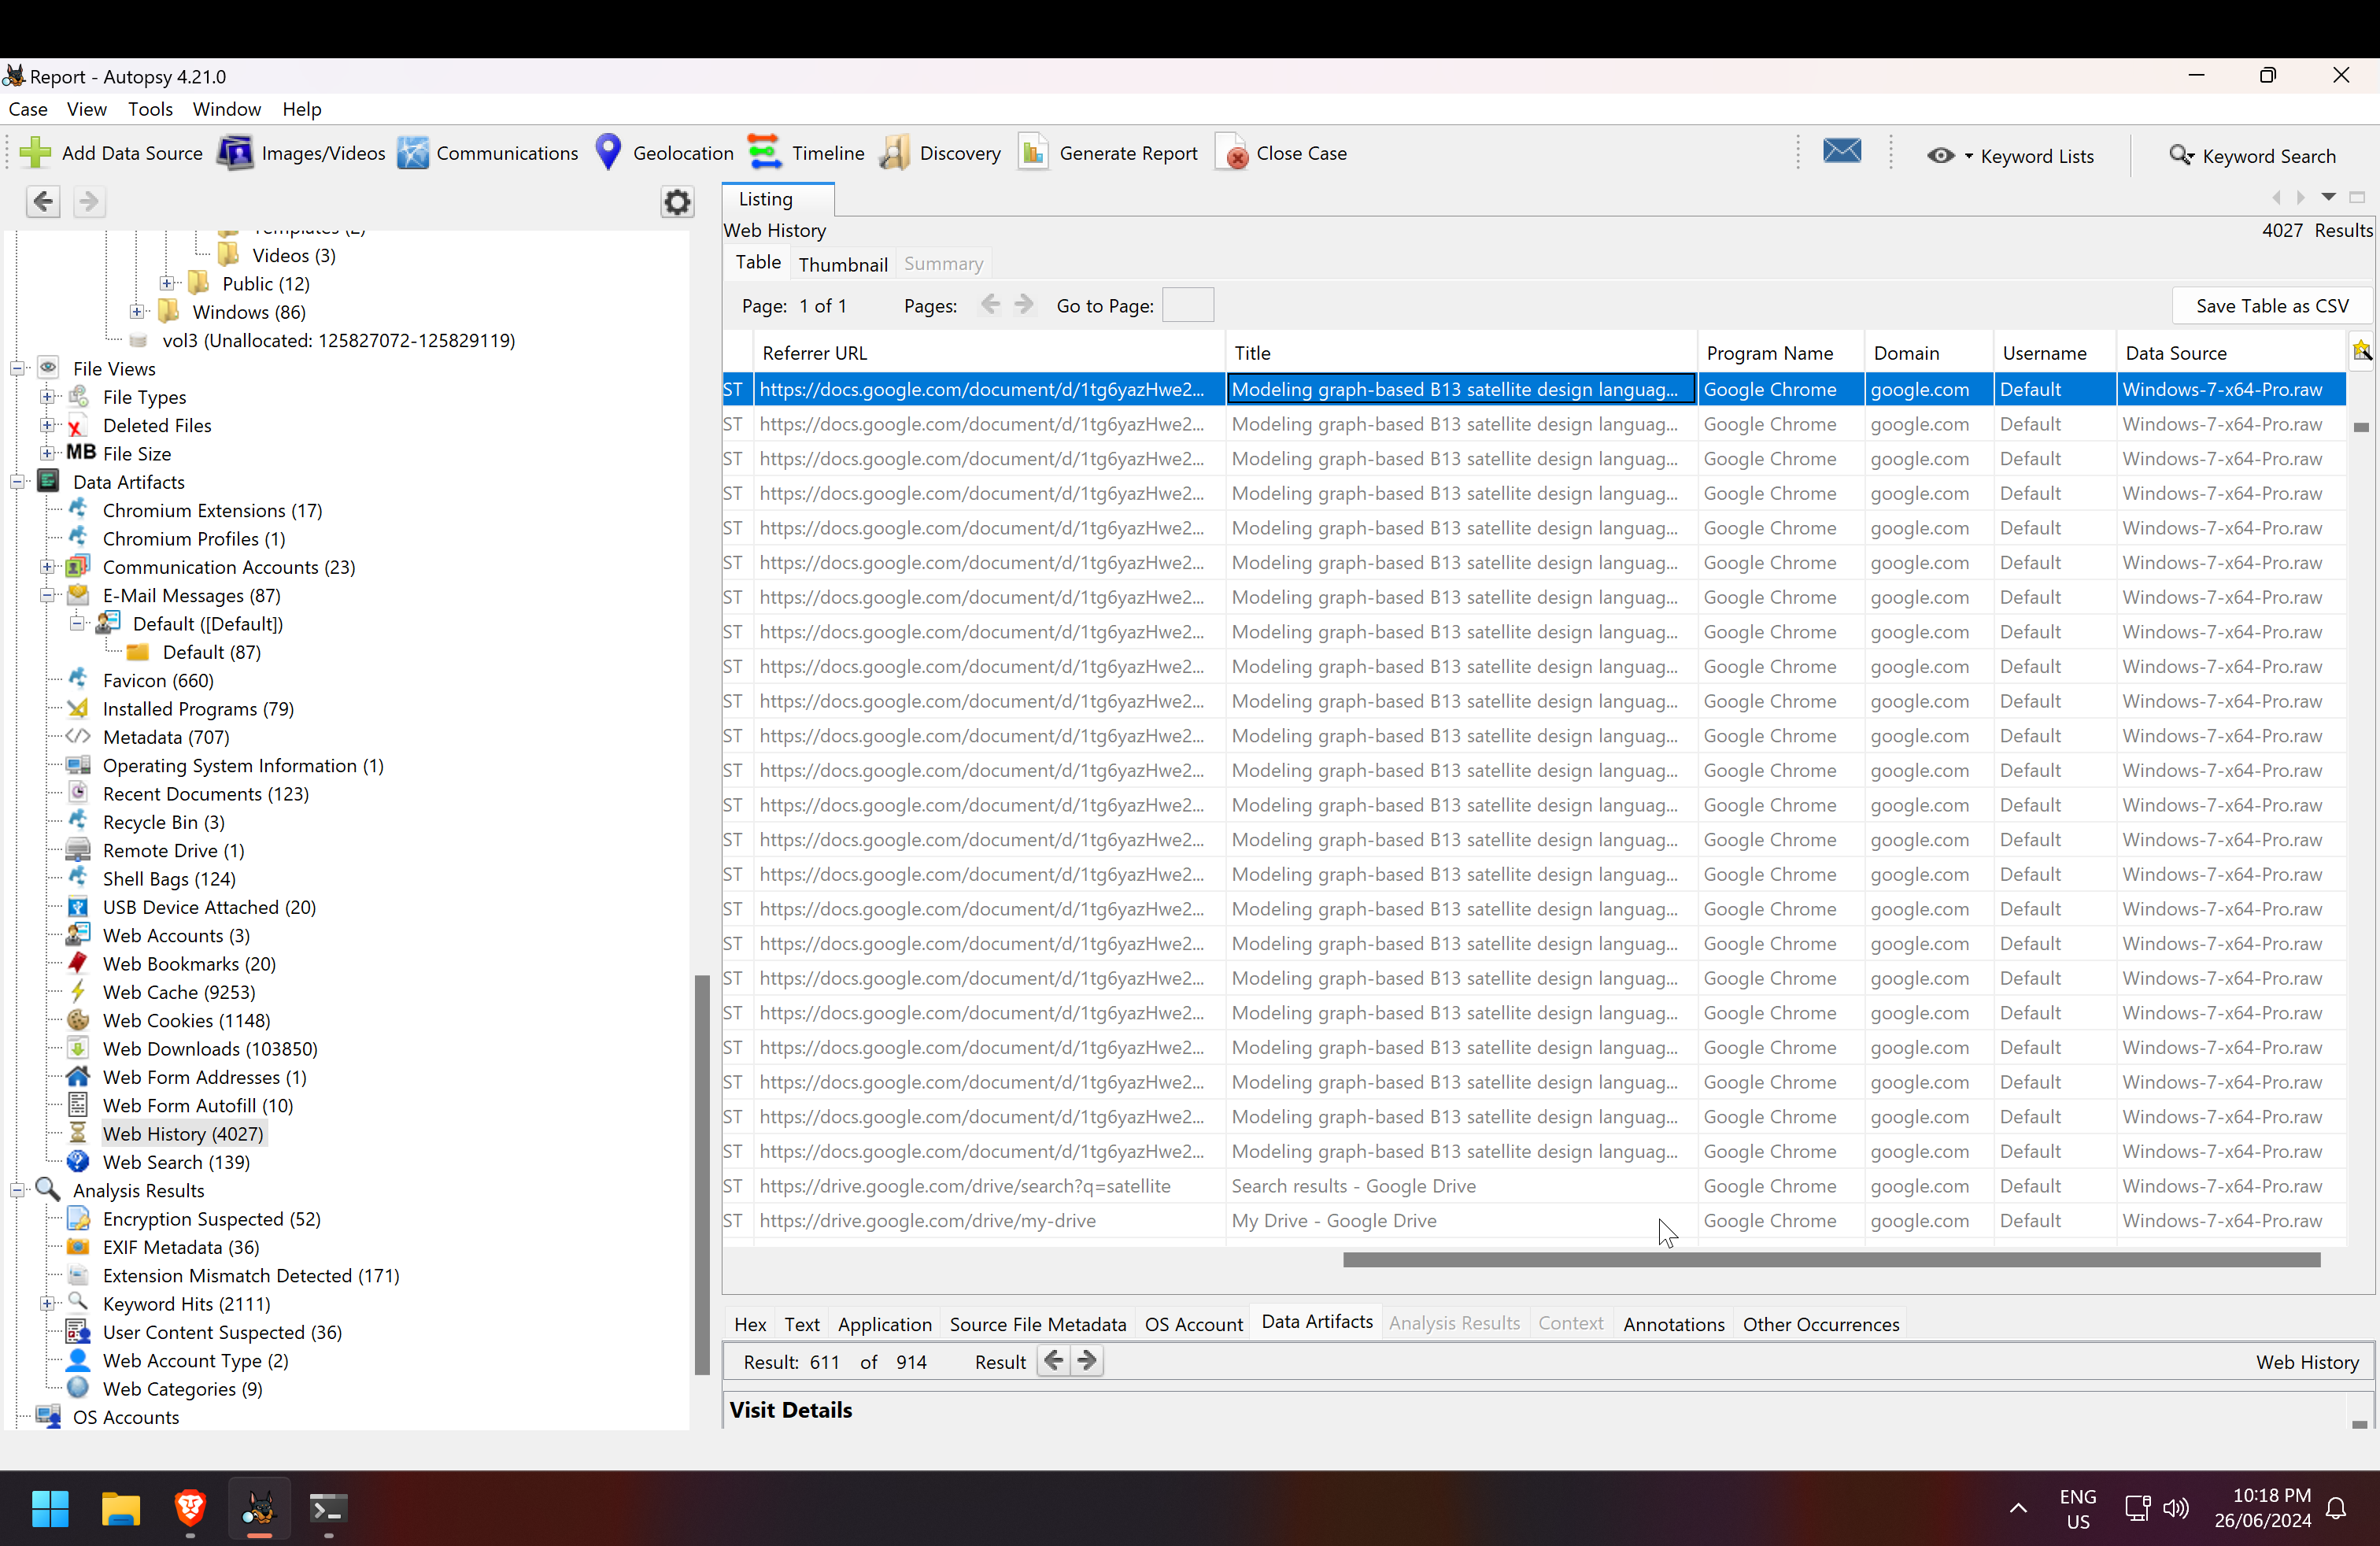
\includegraphics[width=1.0\textwidth]{history6.png}
    \caption{Recent browsing history}
    \label{fig:webhistory}
\end{figure}

\begin{figure}[H]
    \centering
    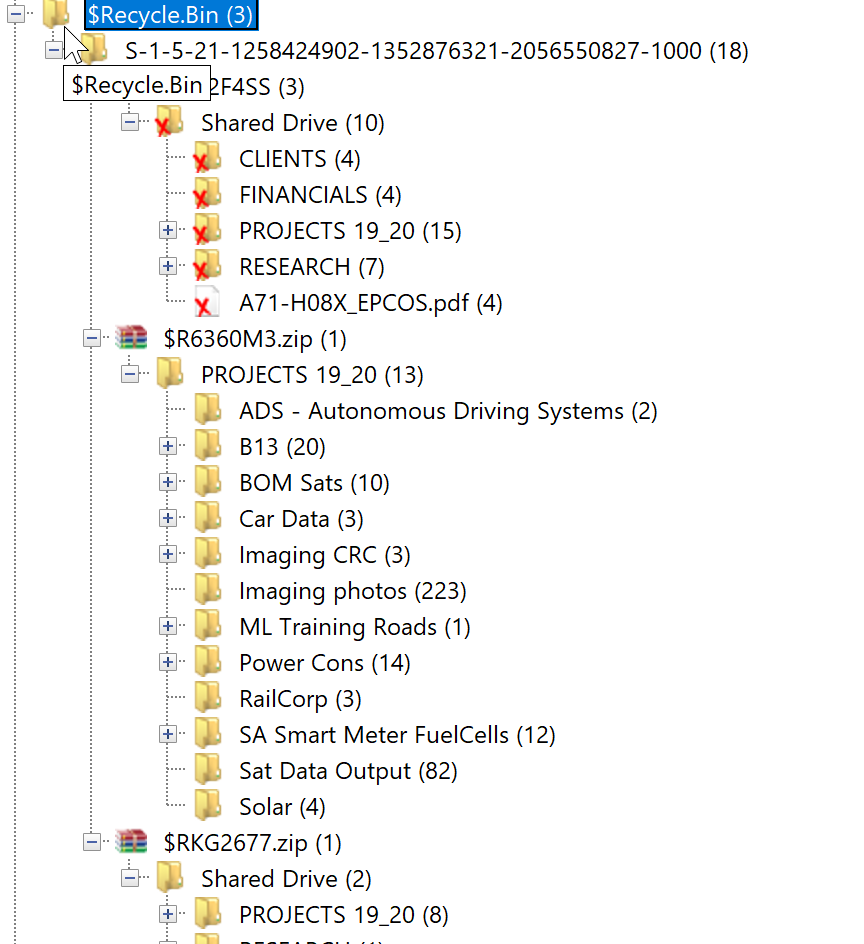
\includegraphics[width=1.0\textwidth]{recycle.png}
    \caption{Recycling bin}
    \label{recycle}
\end{figure}

\begin{figure}[H]
    \centering
    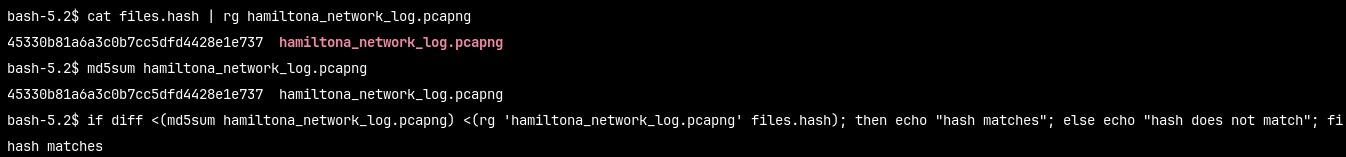
\includegraphics[width=1.0\textwidth]{pcap_verification.png}
    \caption{Cryptographic hash verification of the packet capture file}
    \label{pcap_verification}
\end{figure}

\begin{figure}[H]
    \centering
    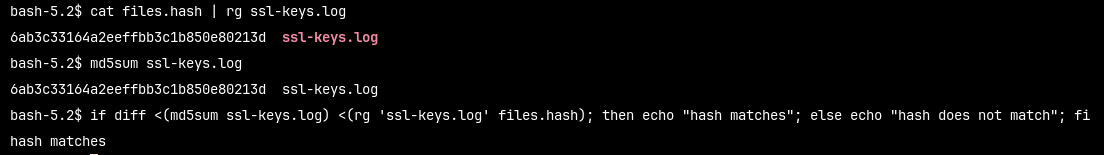
\includegraphics[width=1.0\textwidth]{ssl_key_log_verification.png}
    \caption{Cryptographic hash verification of the SSL key log file}
    \label{ssl_key_log_verification}
\end{figure}

\begin{figure}[H]
    \centering
    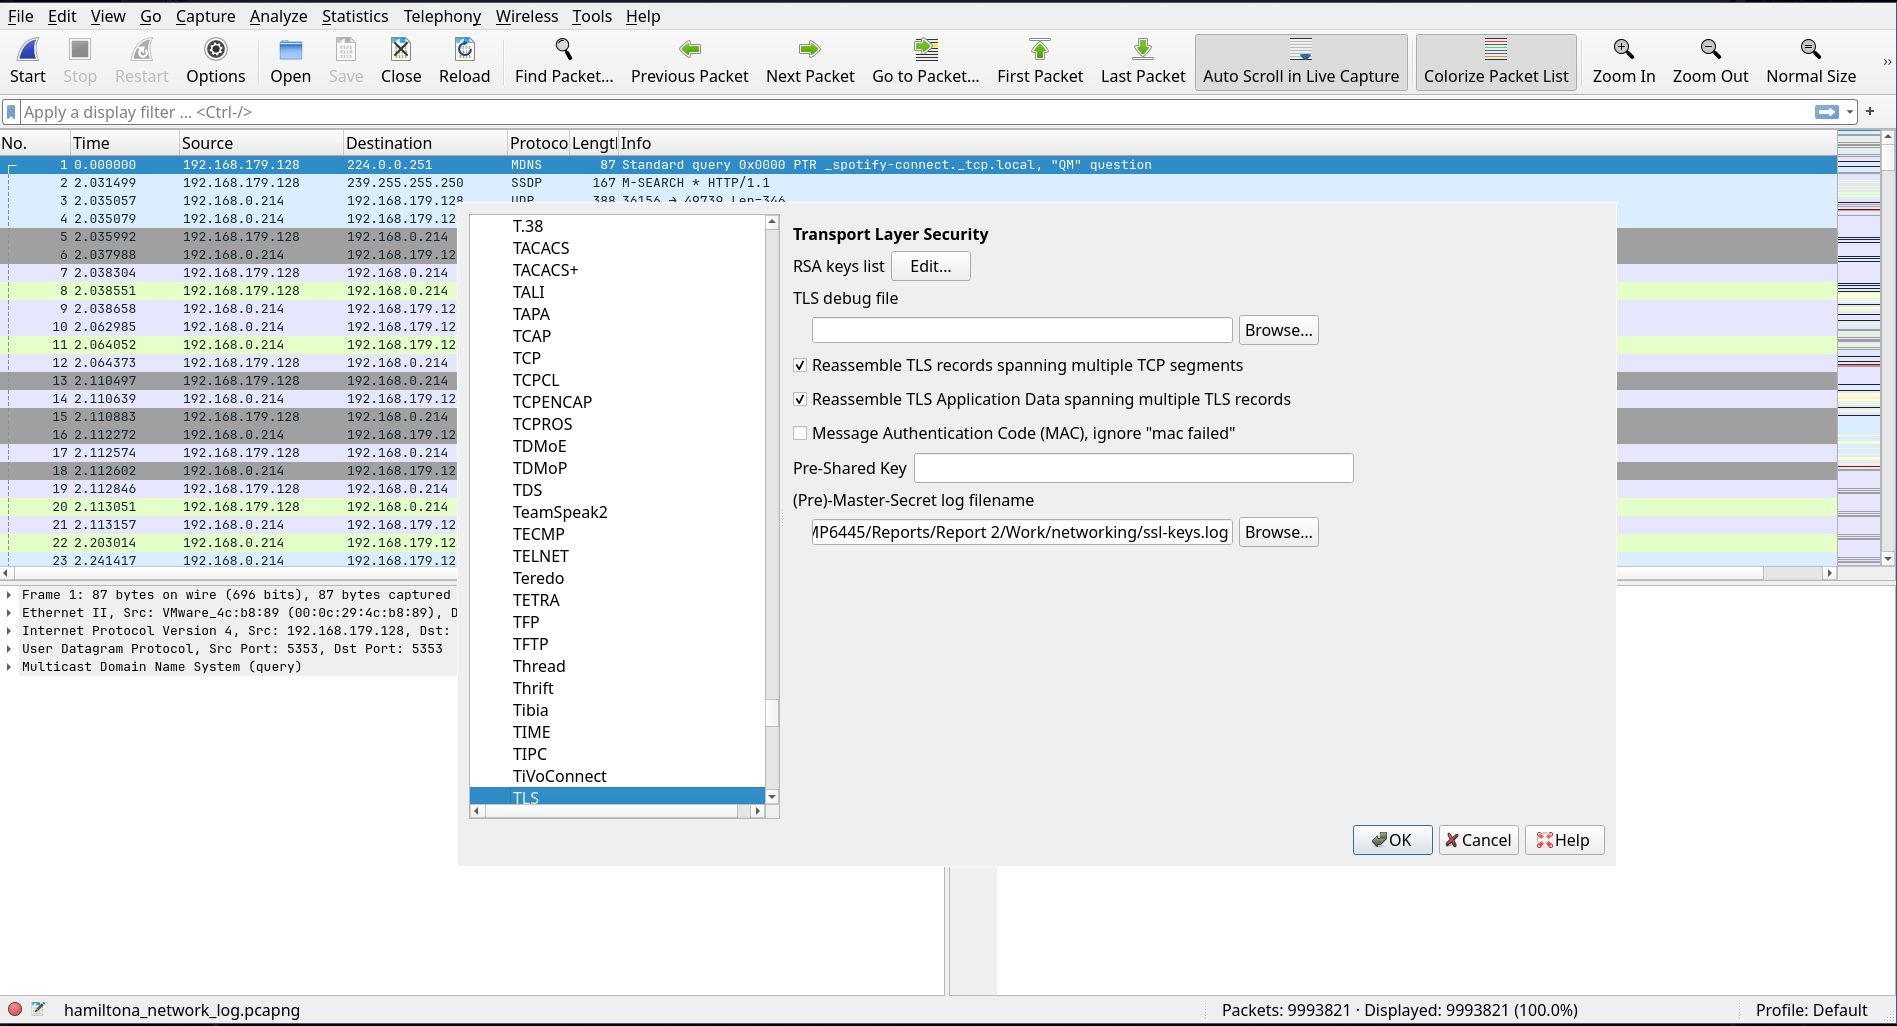
\includegraphics[width=1.0\textwidth]{importing_ssl_key_log.png}
    \caption{Importing the SSL key log to Wireshark}
    \label{importing_ssl_key_log}
\end{figure}

\begin{figure}[H]
    \centering
    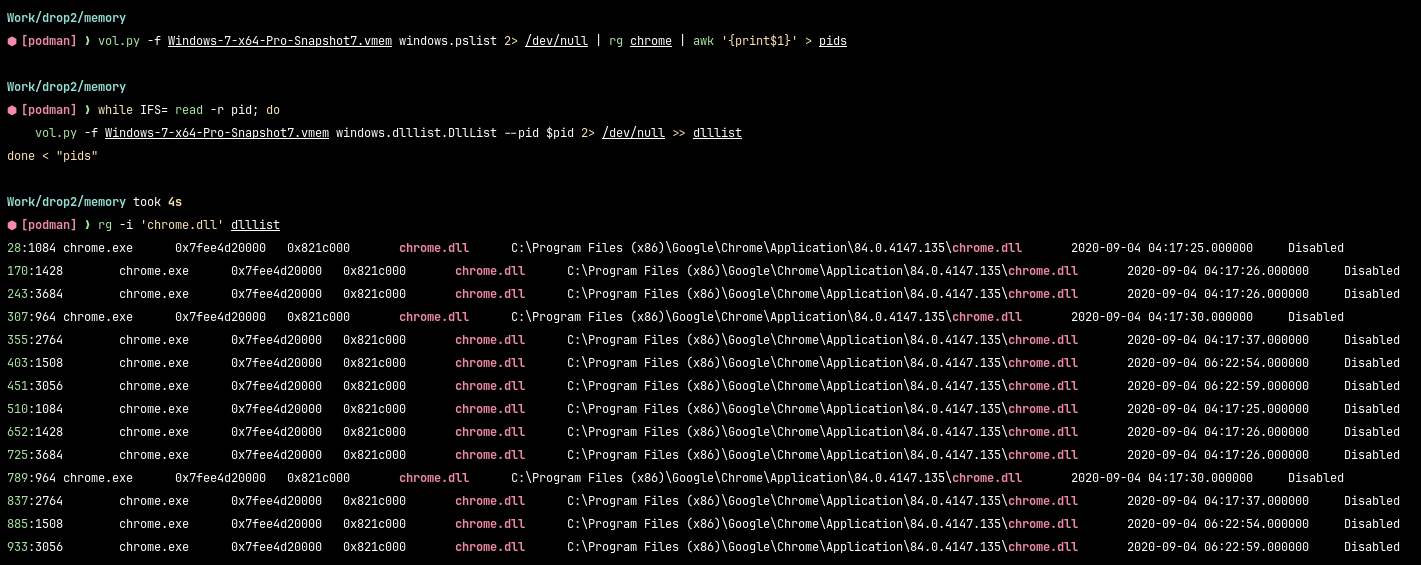
\includegraphics[width=1.0\textwidth]{chrome_version.png}
    \caption{Finding the version of Google Chrome used from the memory dump}
    \label{chrome_version}
\end{figure}

% section Figures (end)

\subsection{Dockerfile for Volatility 3 Environment} % (fold)
\label{sec:Dockerfile for Volatility 3 Environment}
\subsubsection{Dockerfile}
\label{subsubsec:Dockerfile}
\begin{verbatim}
FROM alpine:edge

# Update and install necessary packages
RUN apk update && apk upgrade && apk add --no-cache \
    python3 \
    7zip \
    shadow \
    curl \
    git \
    tmux \
    neovim \
    starship \
    clang \
    zsh \
    bat \
    eza \
    fzf \
    ripgrep \
    fd \
    bind-tools \
    py3-virtualenv \
    termshark \
    traceroute \
    neomutt

# Add a new user
RUN adduser -D COMP6845
RUN usermod -aG wireshark COMP6845
RUN chsh -s /bin/zsh COMP6845

USER COMP6845
WORKDIR /home/COMP6845

# Clone necessary repositories
RUN git clone https://github.com/tmux-plugins/tpm /home/COMP6845/.local/share/tmux/plugins/tpm
RUN git clone https://github.com/zsh-users/zsh-syntax-highlighting.git /home/COMP6845/.local/share/zsh/zsh-syntax-highlighting
RUN git clone https://github.com/zsh-users/zsh-autosuggestions /home/COMP6845/.local/share/zsh/zsh-autosuggestions
RUN git clone https://github.com/Aloxaf/fzf-tab /home/COMP6845/.local/share/zsh/fzf-tab

# Set up volatility
RUN mkdir -p /home/COMP6845/.local/bin
WORKDIR /home/COMP6845/.local/bin
RUN python3 -m venv volatility
RUN ./volatility/bin/pip install --upgrade pip
RUN ./volatility/bin/pip install volatility3

WORKDIR /home/COMP6845
RUN echo "alias 'vol.py'='/home/COMP6845/.local/bin/volatility/bin/vol'" >> .zshrc

# Create Mail directory and copy mbox files
RUN mkdir -p /home/COMP6845/Mail
COPY --chown=COMP6845:COMP6845 Emails/Harris/all.mbox /home/COMP6845/Mail/harris.mbox
COPY --chown=COMP6845:COMP6845 Emails/Hamilton/all.mbox /home/COMP6845/Mail/hamilton.mbox

# Configure NeoMutt
RUN echo 'set mbox_type=mbox' >> /home/COMP6845/.neomuttrc
RUN echo 'set folder=~/Mail' >> /home/COMP6845/.neomuttrc
RUN echo 'mailboxes ~/Mail/hamilton.mbox ~/Mail/harris.mbox' >> /home/COMP6845/.neomuttrc
RUN echo 'set spoolfile=~/Mail/hamilton.mbox' >> /home/COMP6845/.neomuttrc

CMD ["zsh"]
\end{verbatim}

\subsubsection{zshrc}
\label{subsubsec:zshrc}

\begin{verbatim}
# Lines configured by zsh-newuser-install
HISTFILE=~/.histfile
HISTSIZE=1000
SAVEHIST=1000
bindkey -e
# End of lines configured by zsh-newuser-install
# The following lines were added by compinstall
zstyle :compinstall filename '/home/COMP3141/.zshrc'

autoload -Uz compinit
compinit
# End of lines added by compinstall

alias vim=nvim
alias v=nvim

alias cat=bat

alias ls='eza --icons'
alias ll='eza --icons -l'
alias la='eza --icons -la'

# Plugins
source ~/.local/share/zsh/zsh-syntax-highlighting/zsh-syntax-highlighting.zsh
source ~/.local/share/zsh/zsh-autosuggestions/zsh-autosuggestions.zsh
source ~/.local/share/zsh/fzf-tab/fzf-tab.plugin.zsh

# Start starship
# ~/.zshrc
eval "$(starship init zsh)"
\end{verbatim}

\subsubsection{Instructions for use}

Install and set up Docker or Podman. Then:

\begin{enumerate}
    \item Create a new, empty directory and change into said directory.
    \item Copy the contents of Section~\ref{subsubsec:Dockerfile} into a file named \texttt{Dockerfile} in the current working directory.
    \item Copy the contents of Section~\ref{subsubsec:zshrc} intto a file named \texttt{.zshrc} in the current working directory.
    \item Execute the following command to build the container image: \texttt{docker build -t comp6845-report2 .}
    \item Execute the following command to initialise a new container from the image that was previously built and enter it: \texttt{docker run -it --name=COMP6845-Report2 comp6845-report2 zsh}
\end{enumerate}

% section Dockerfile for Volatility 3 Environment (end)

% \addcontentsline{toc}{section}{Acknowledgements}

%% References
% \bibliographystyle{unsrtnat} % Vancouver reference style (numbering). 
% \bibliographystyle{agsm} % Harvard reference style (author-year). 
% \bibliography{B_bibs/bibliography}
% \addcontentsline{toc}{section}{Bibliography}

%% Appendices
% \input{Addendum/Declaration}
% \addcontentsline{toc}{section}{Declaration}
% \section{Appendix}
\subsection{Figures} % (fold)
\label{sec:Figures}

\begin{figure}[H]
    \centering
    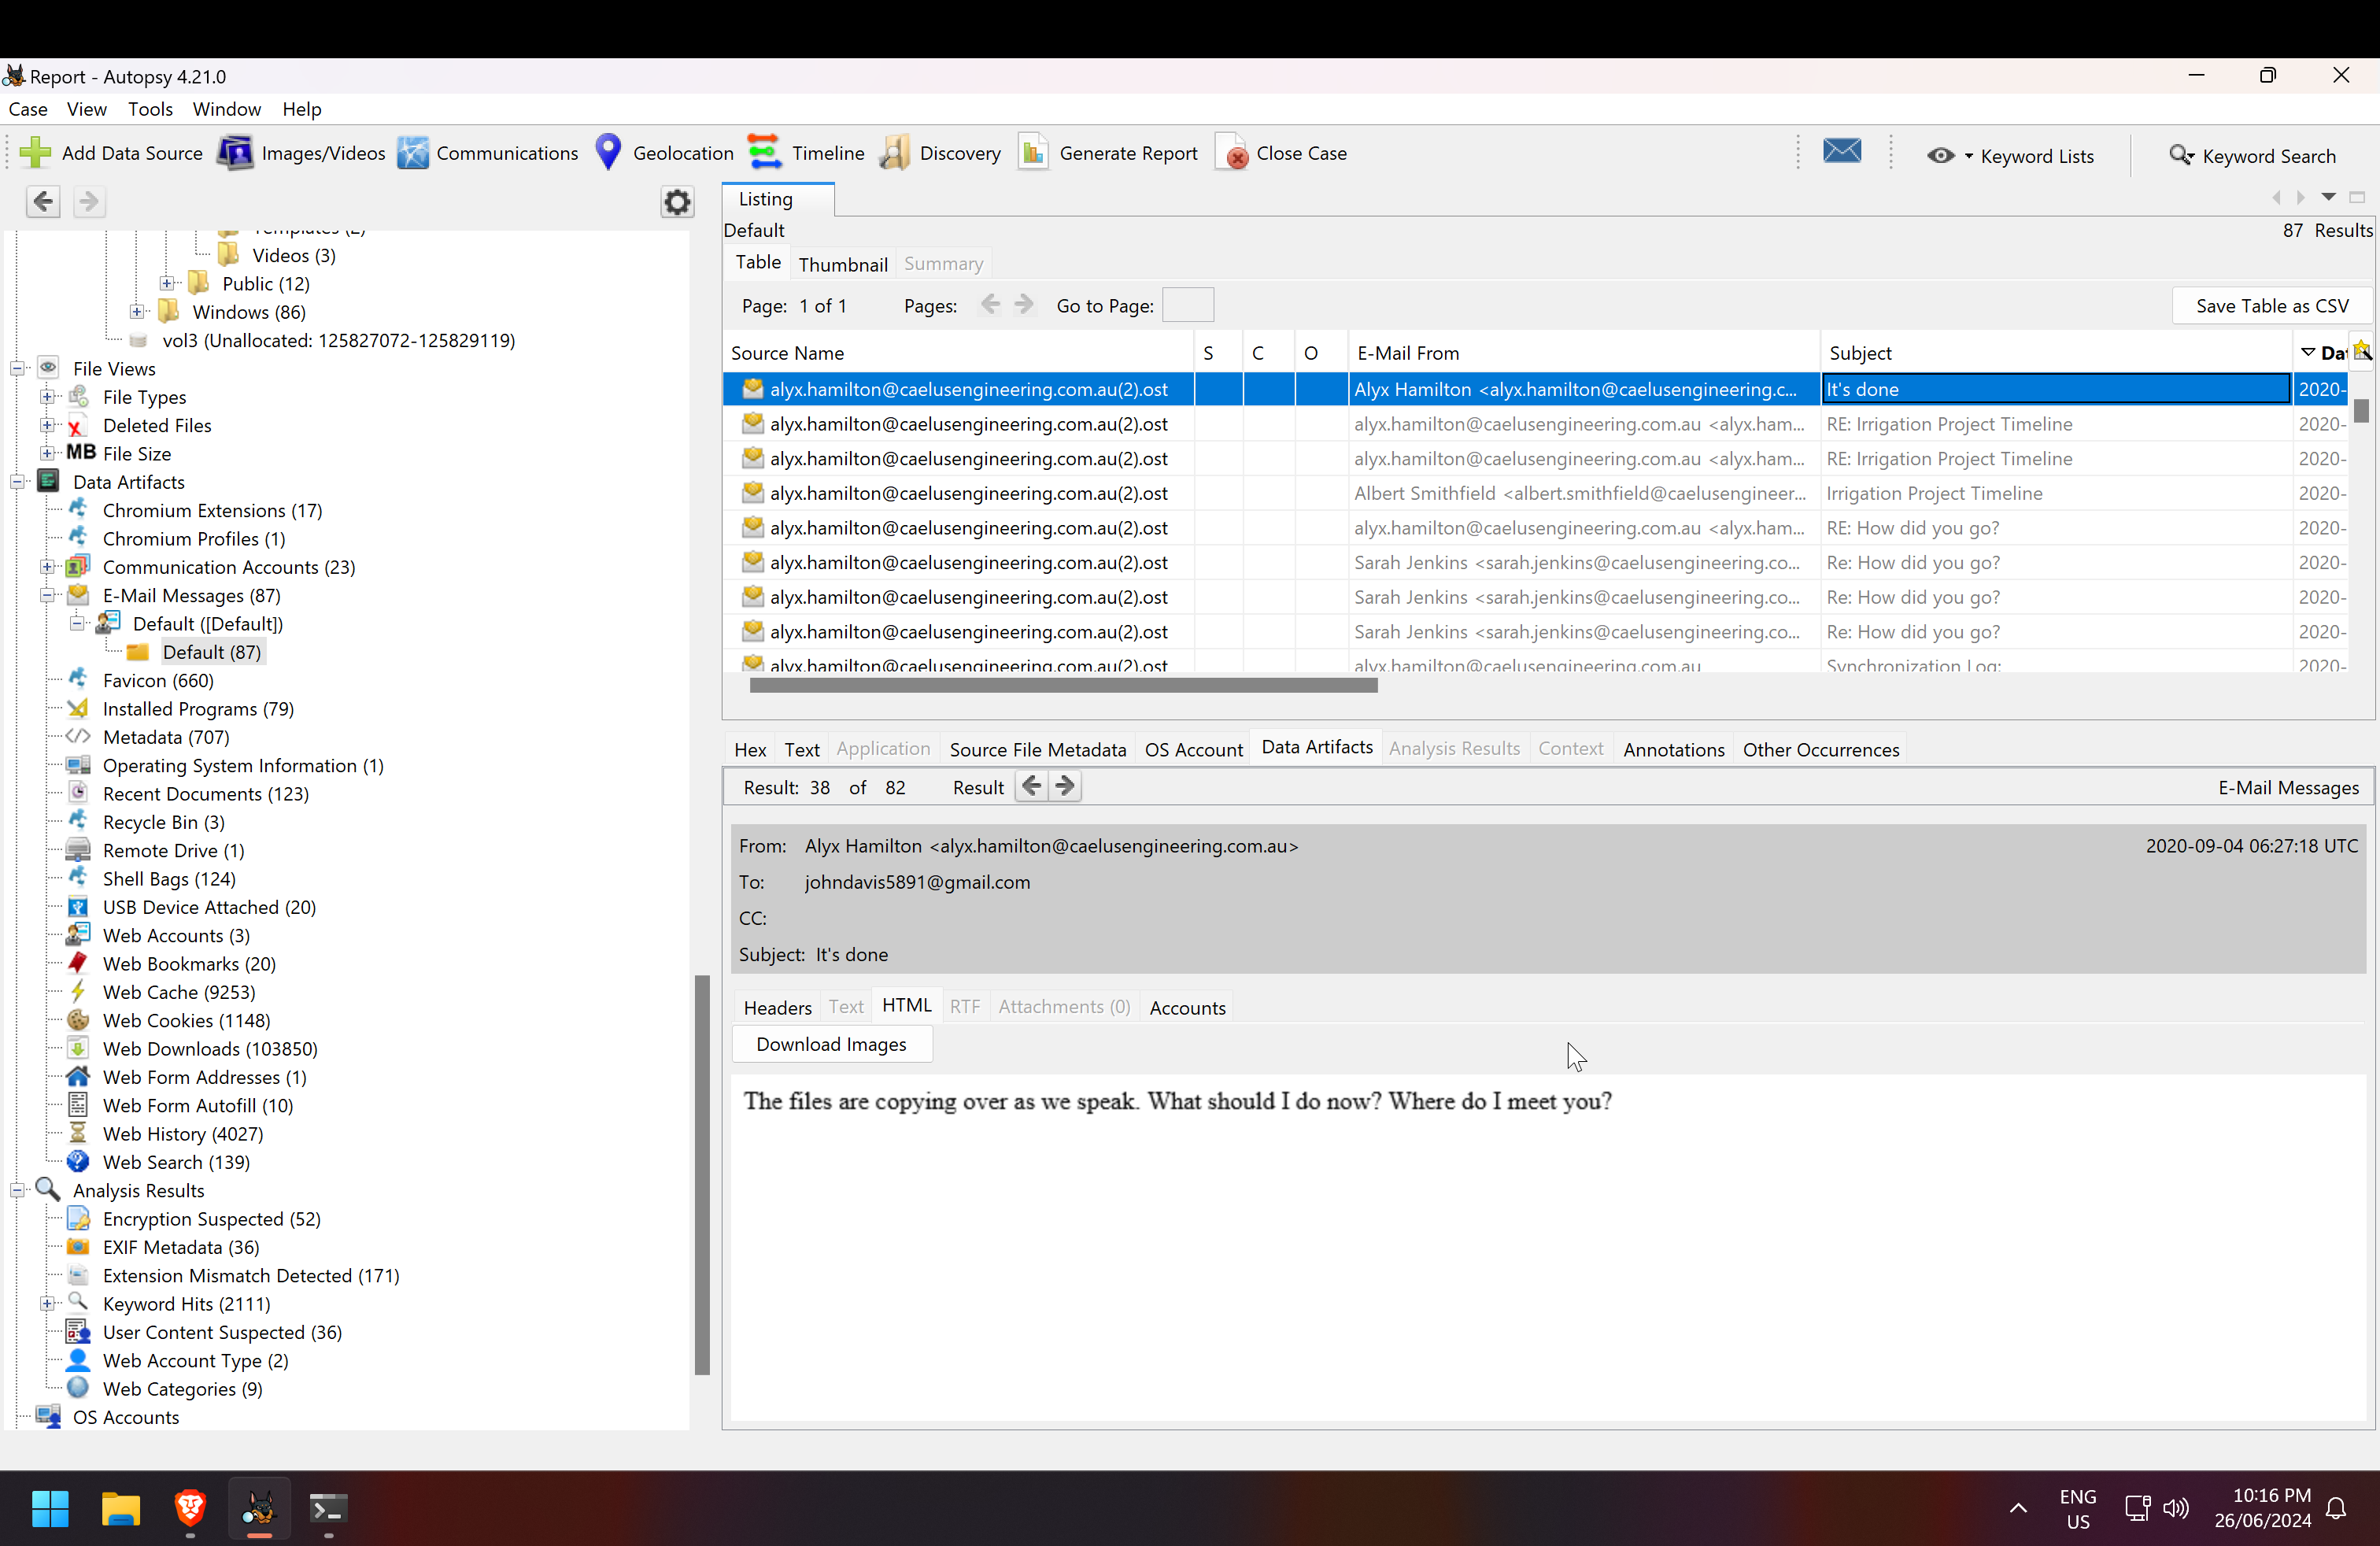
\includegraphics[width=1.0\textwidth]{email.png}
    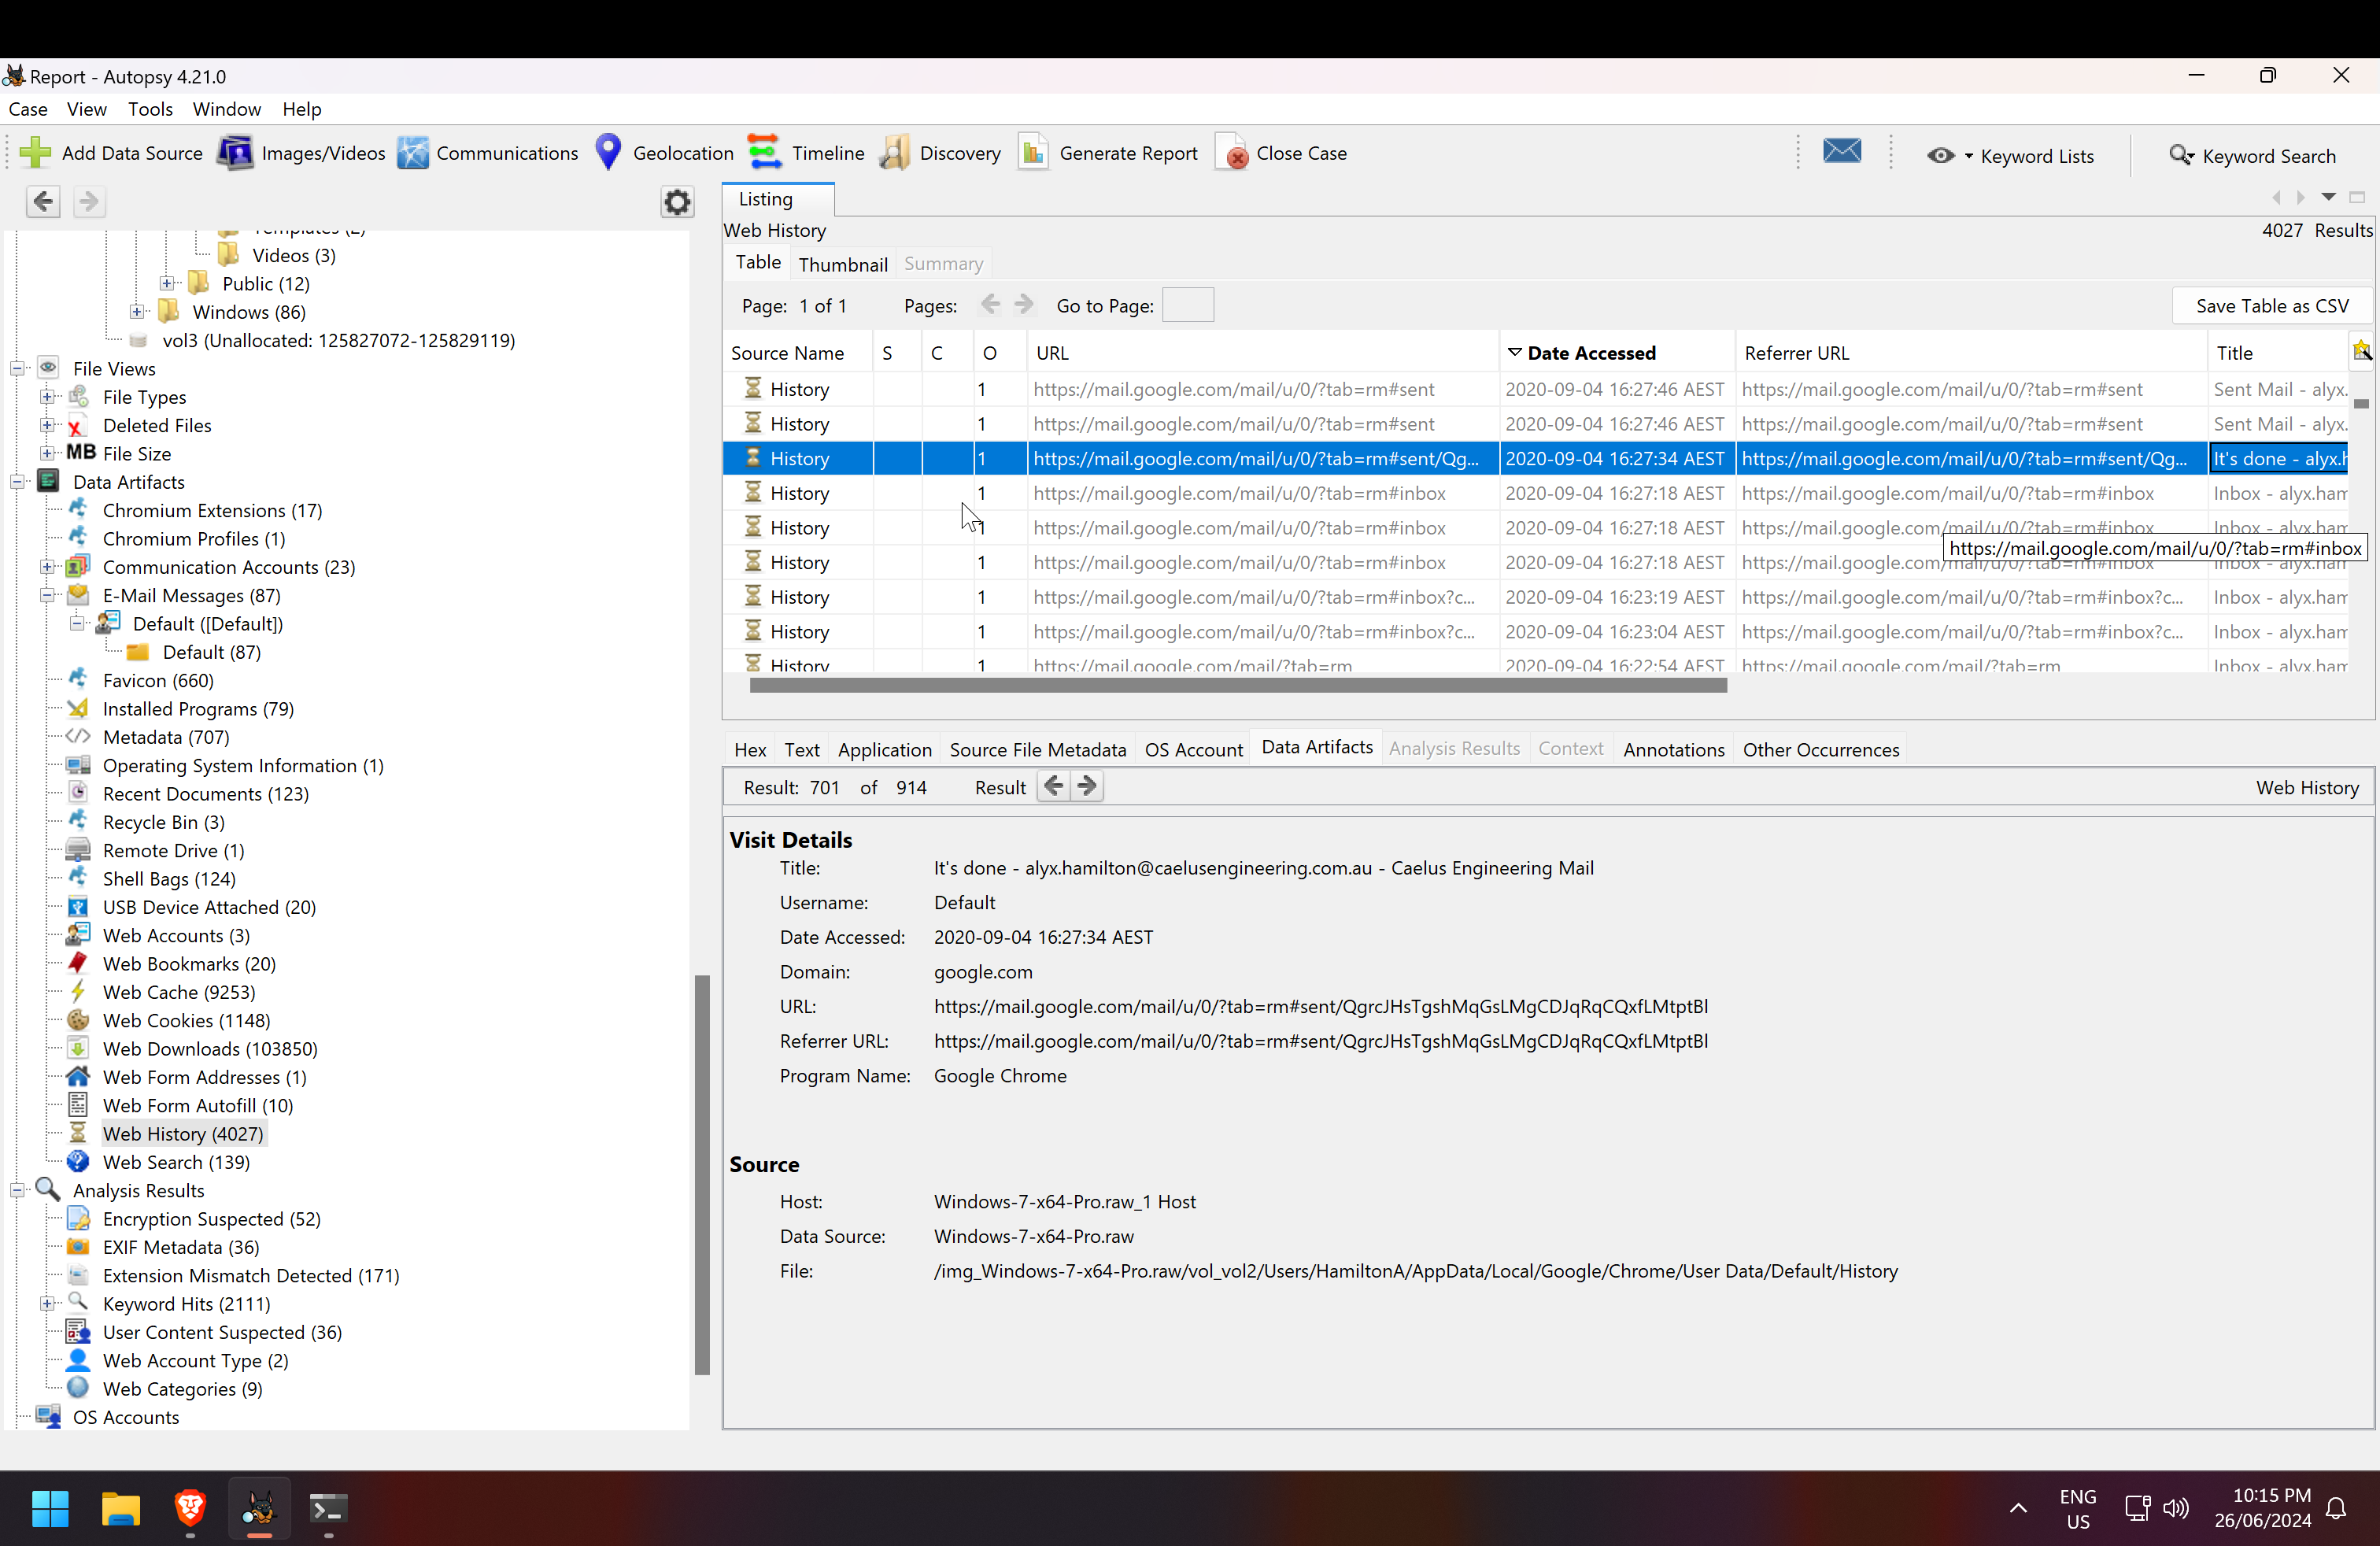
\includegraphics[width=1.0\textwidth]{email_browse_history.png}
    \caption{Cryptic email}
    \label{fig:email}
\end{figure}

\begin{figure}[H]
    \centering
    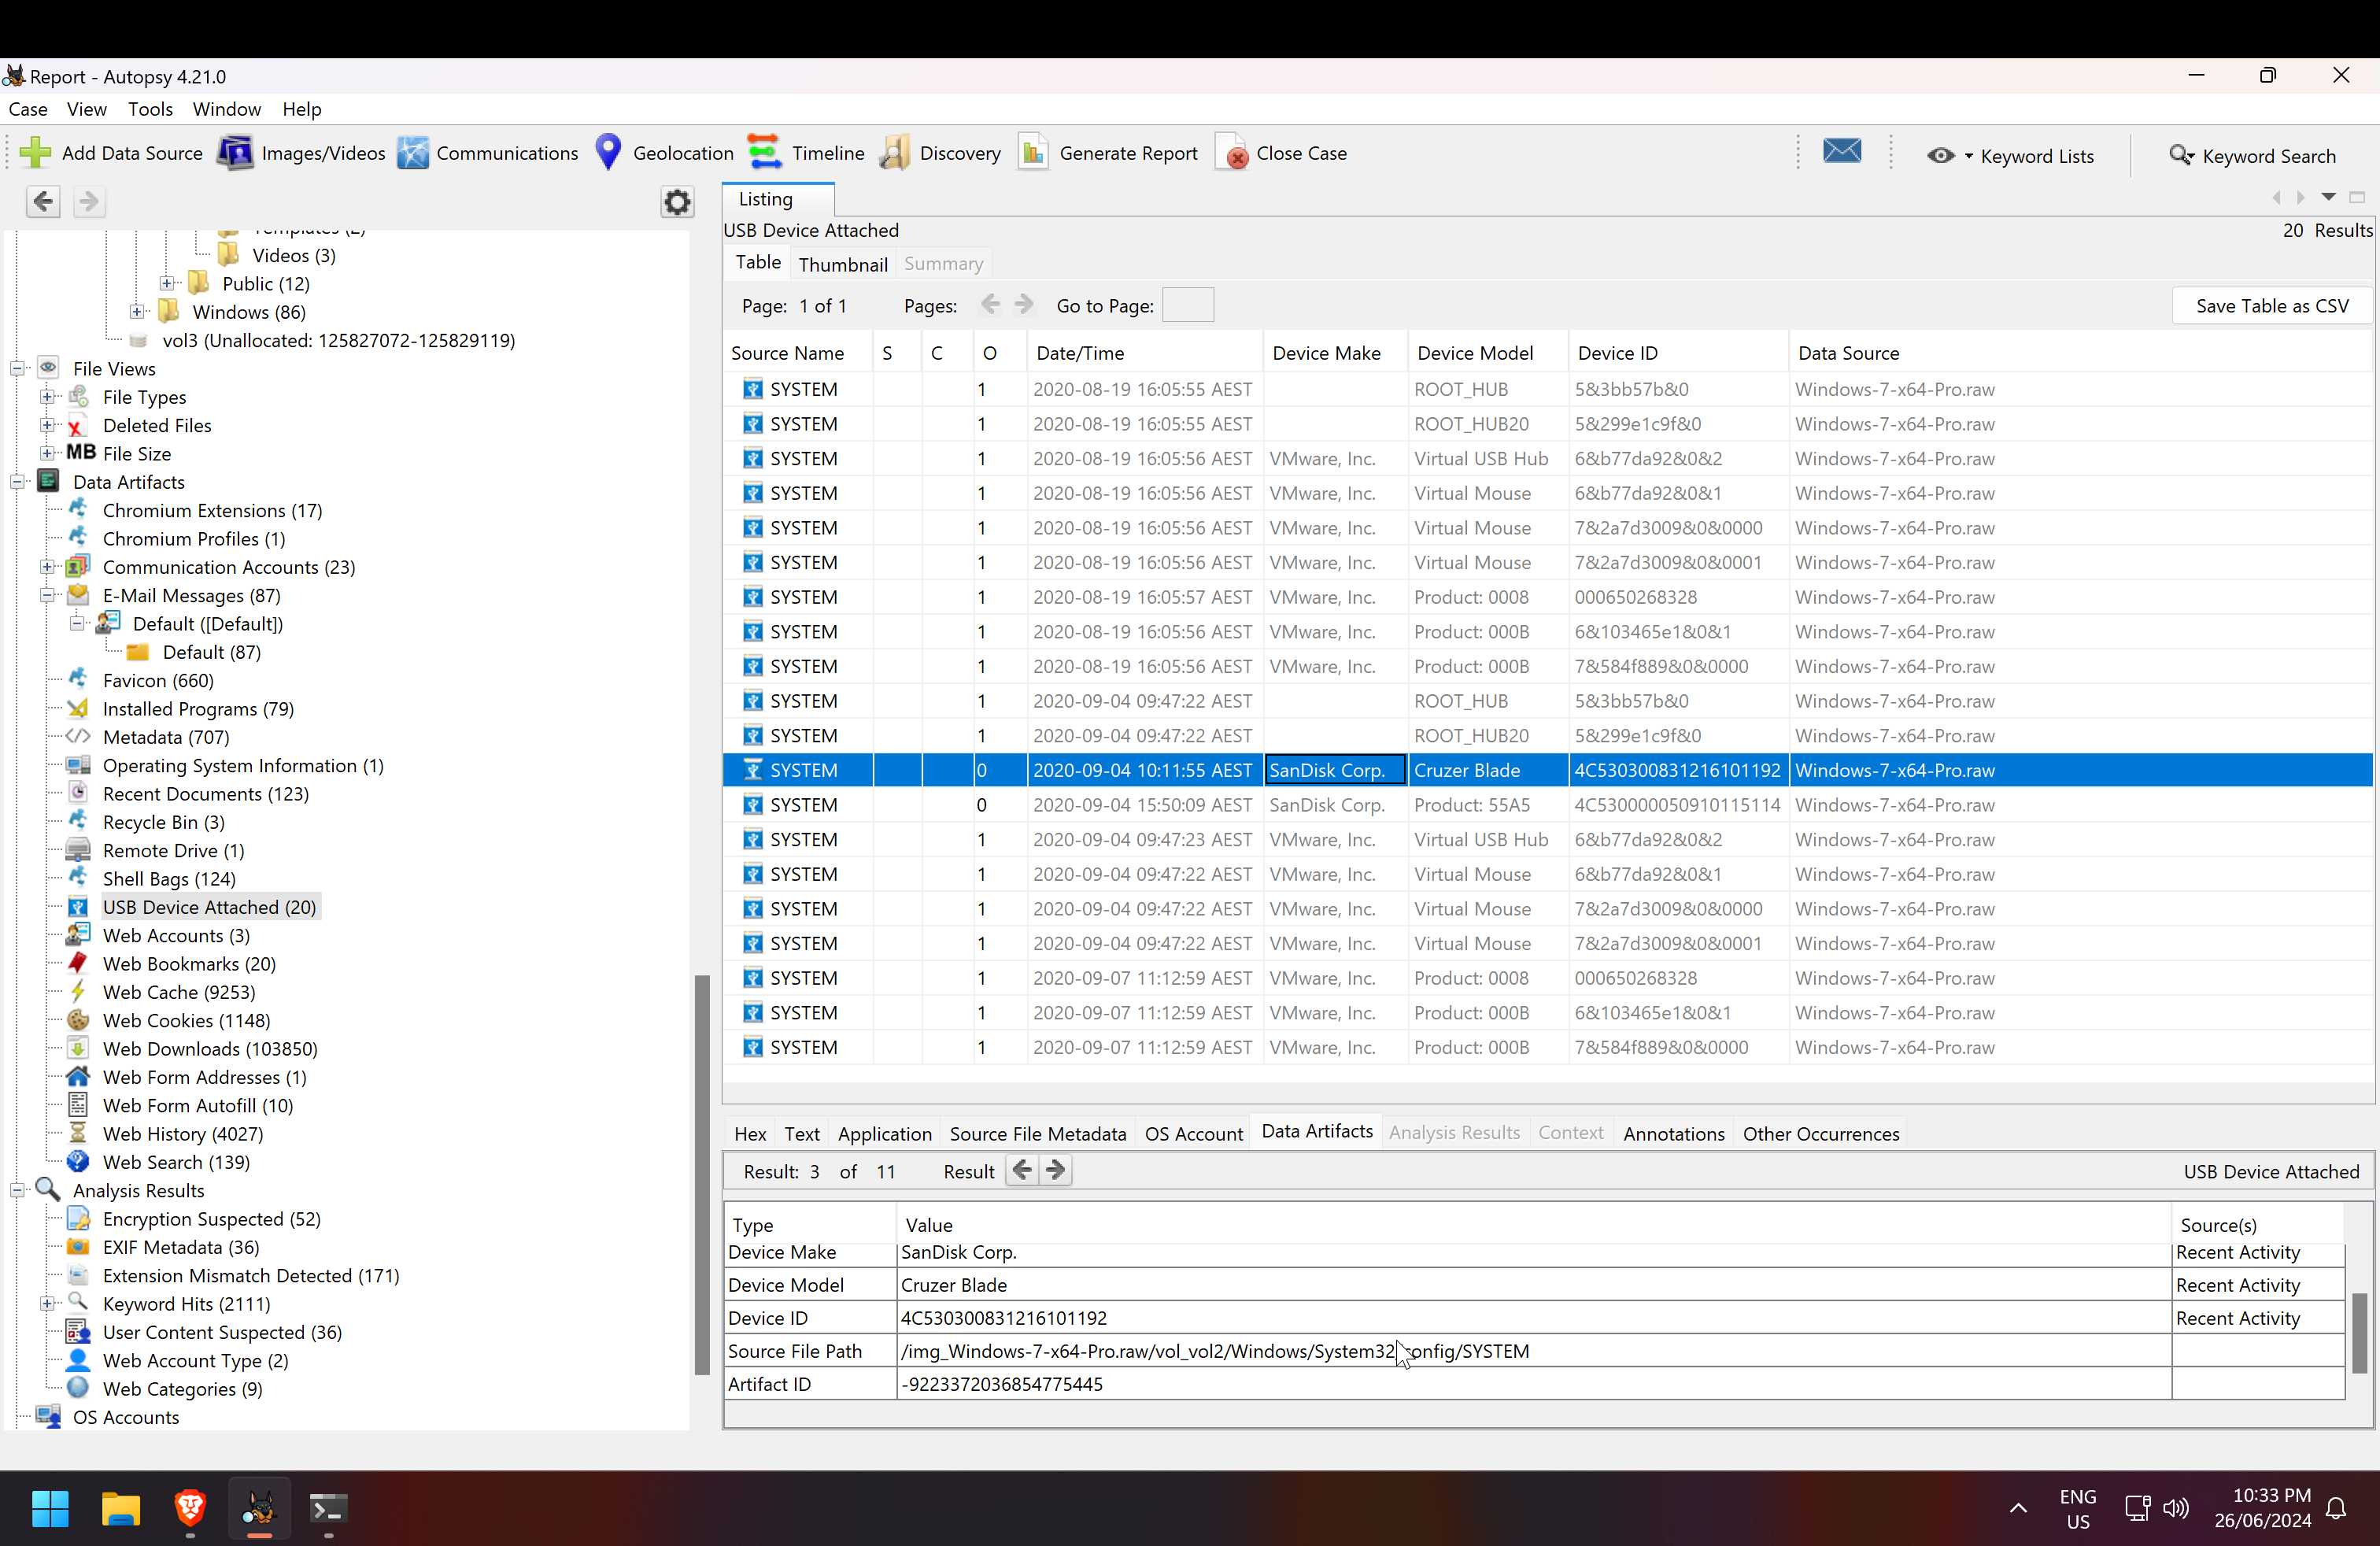
\includegraphics[width=1.0\textwidth]{usb1.png}
    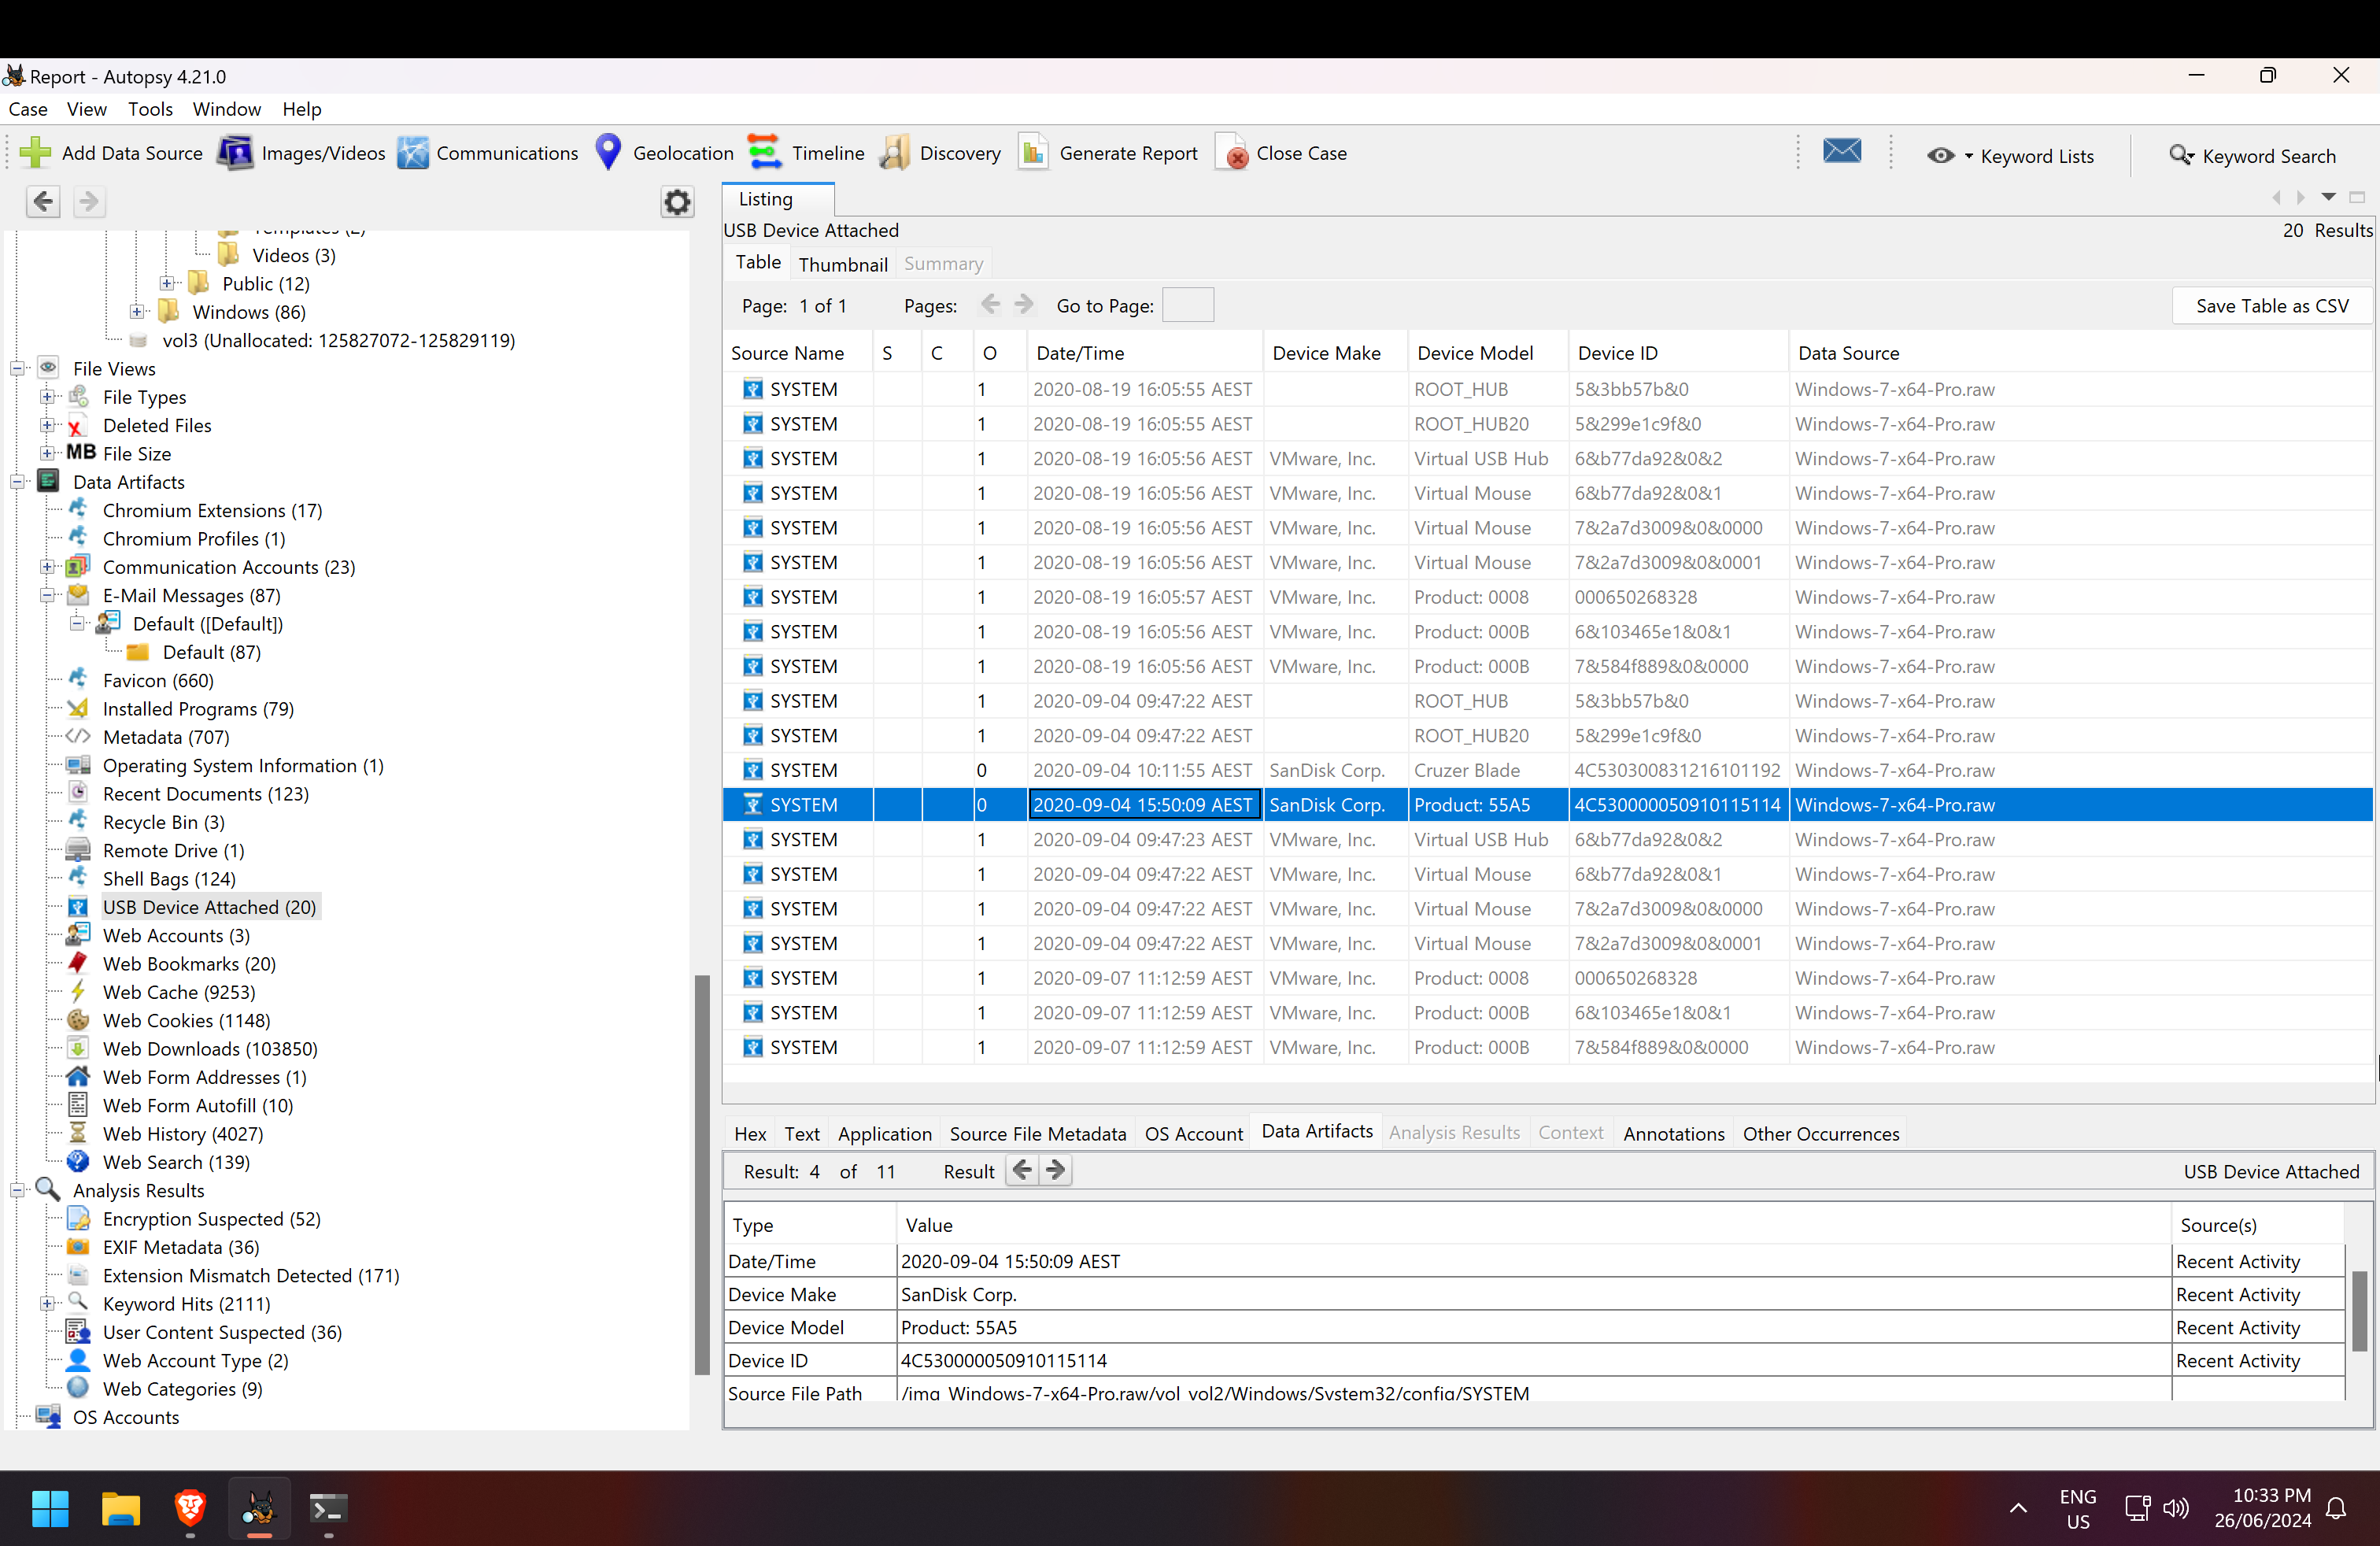
\includegraphics[width=1.0\textwidth]{usb2.png}
    \caption{Attached USB drives}
    \label{fig:usb}
\end{figure}

\begin{figure}[H]
    \centering
    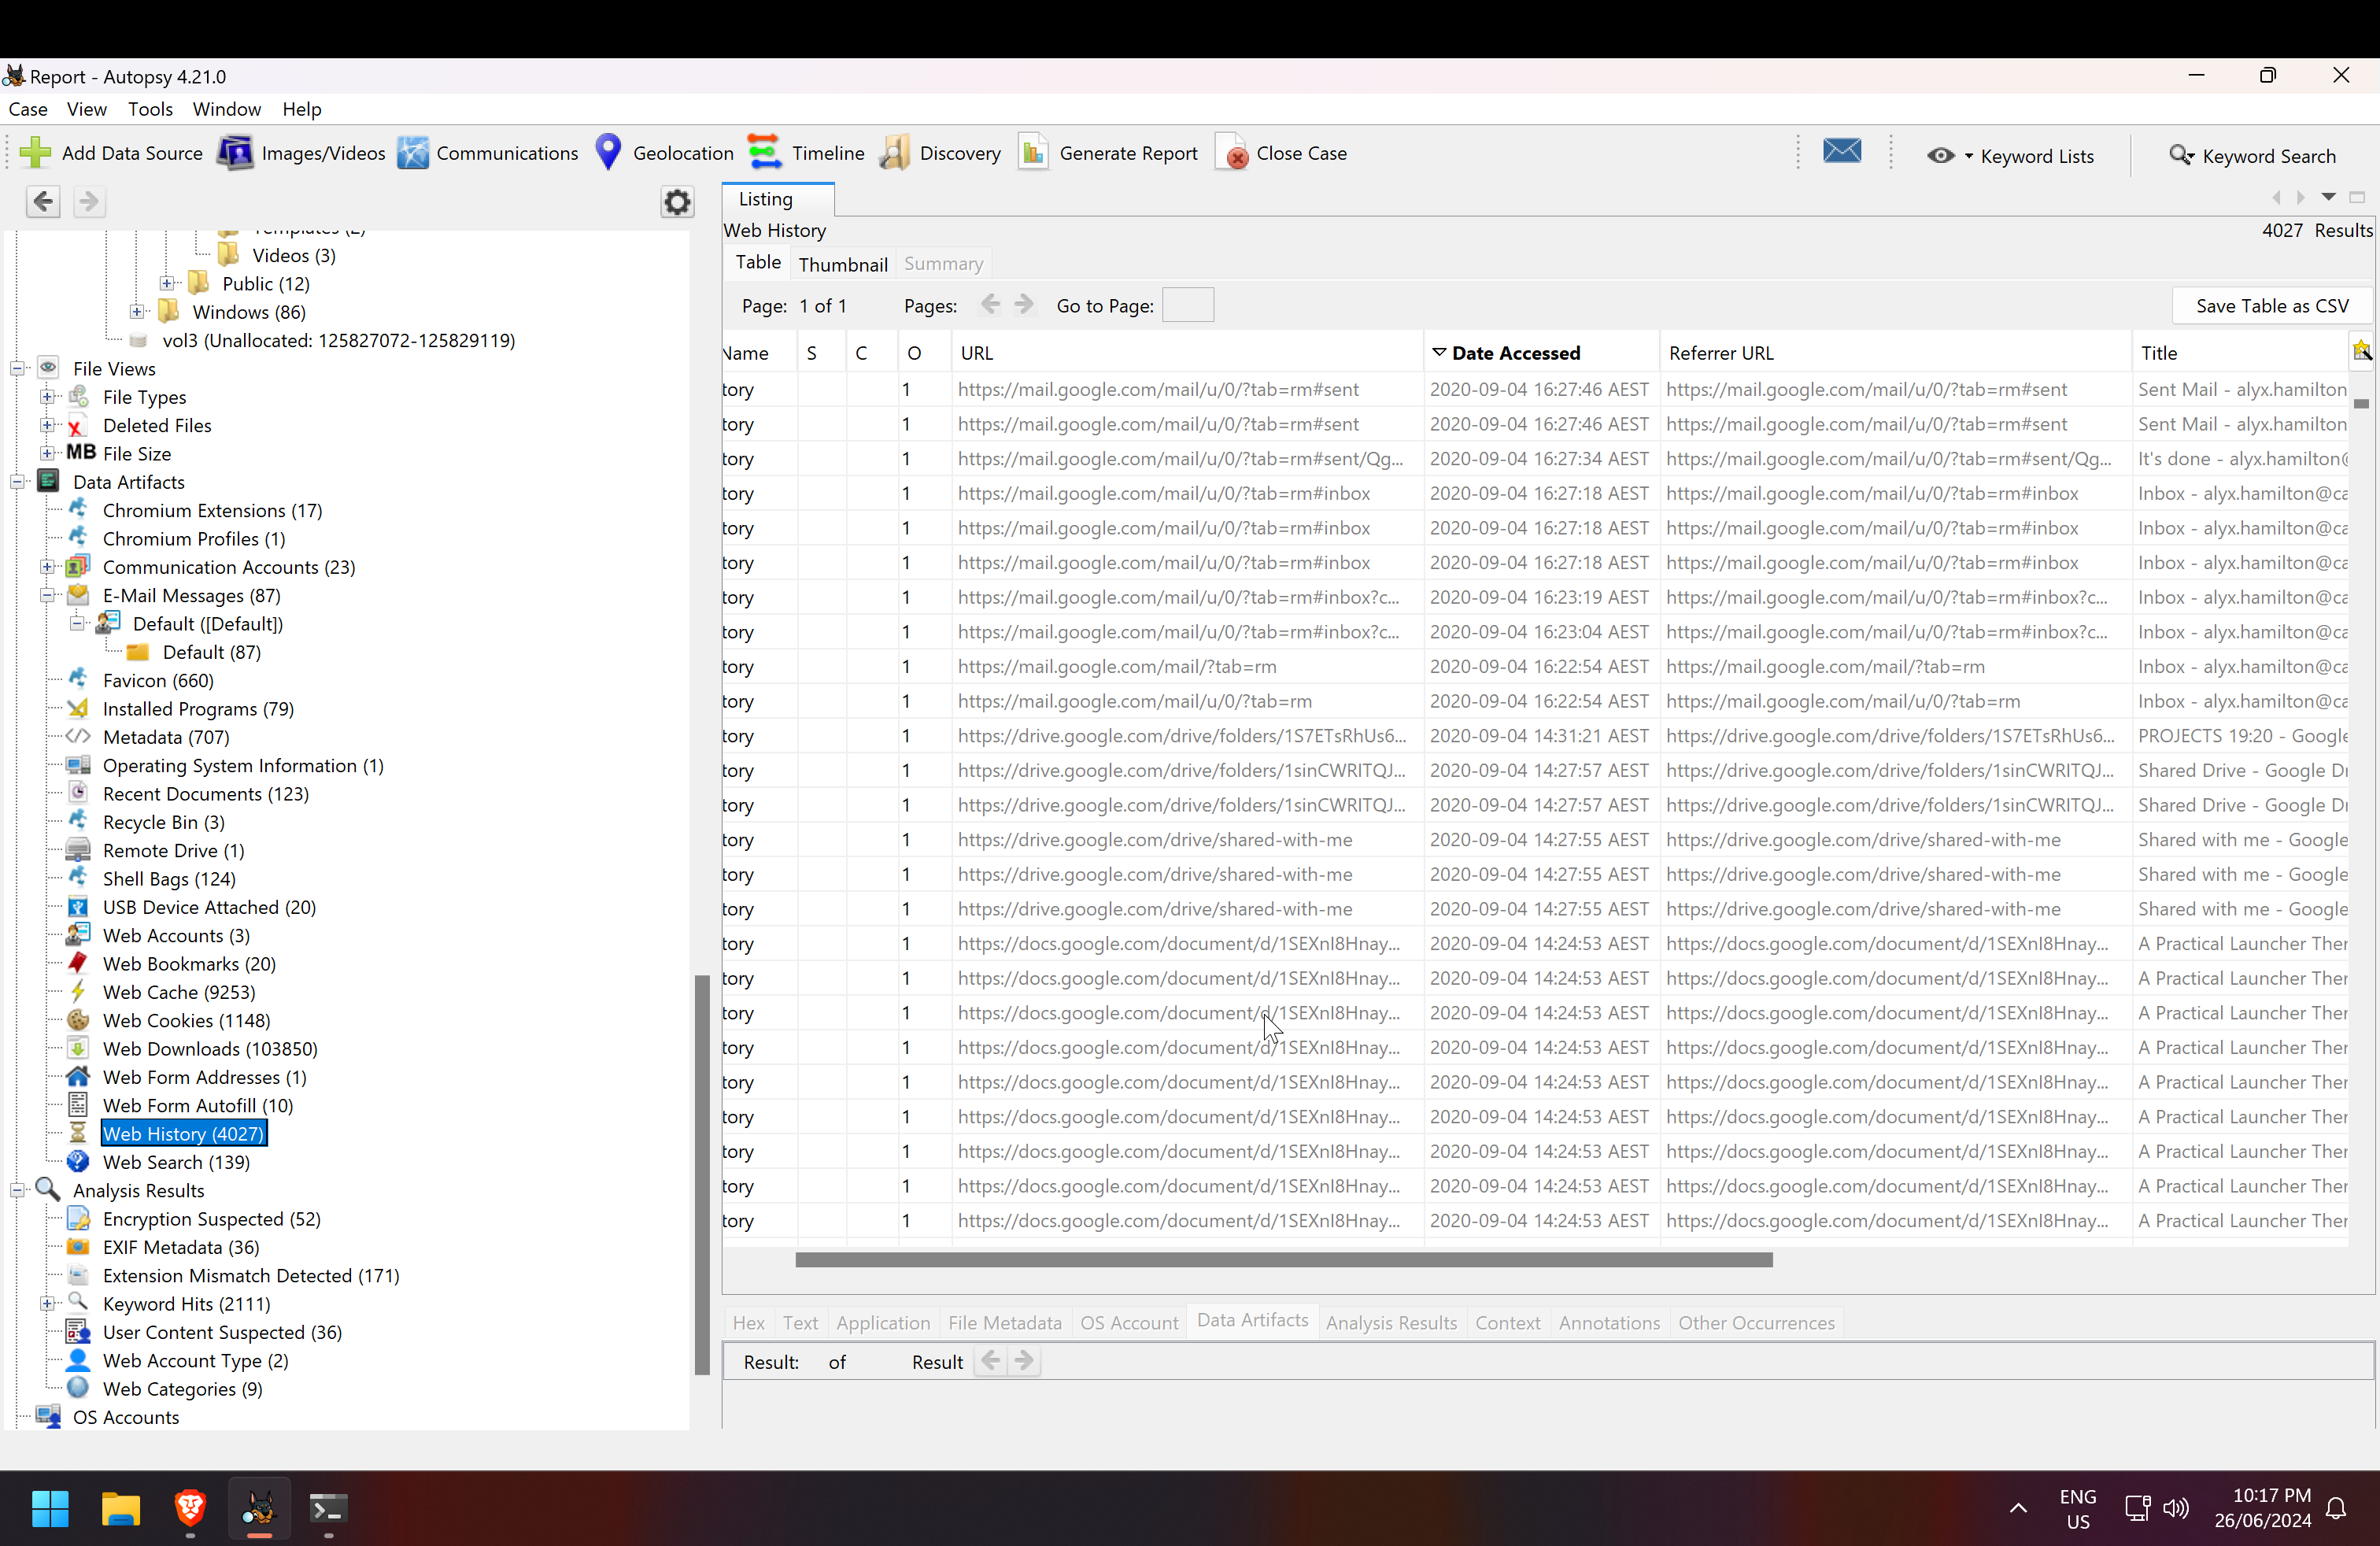
\includegraphics[width=1.0\textwidth]{history1.png}
    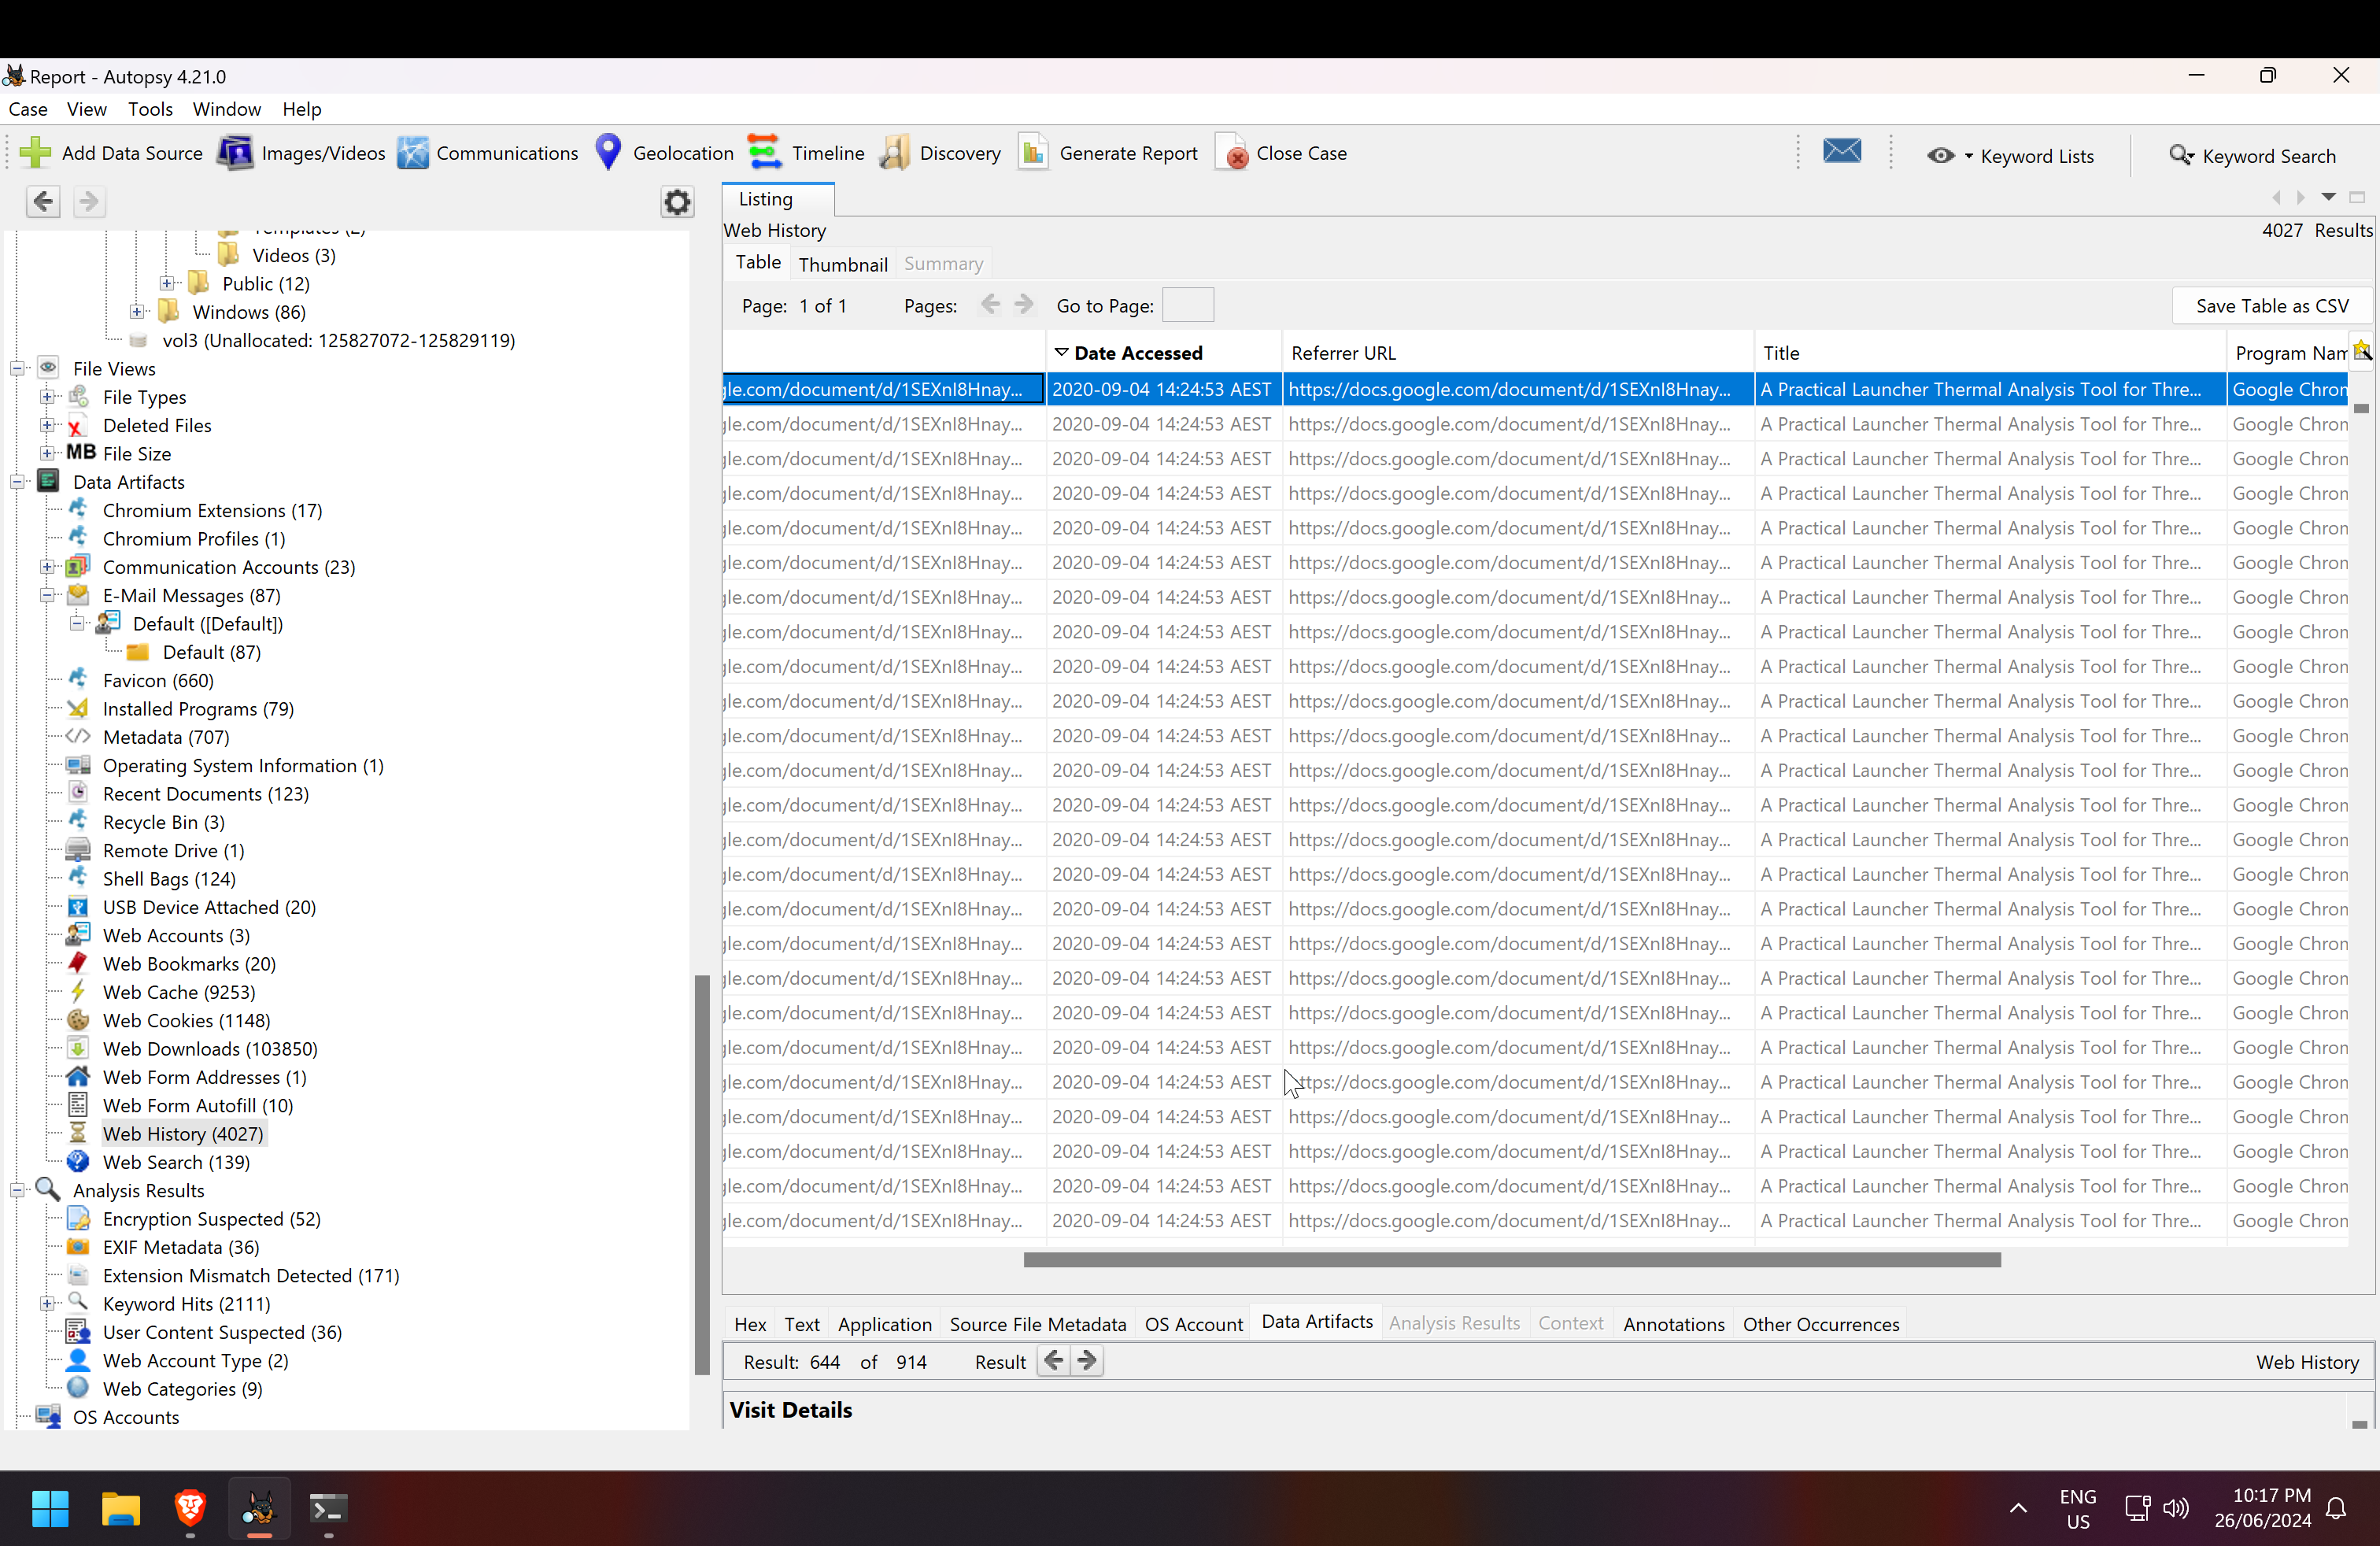
\includegraphics[width=1.0\textwidth]{history2.png}
    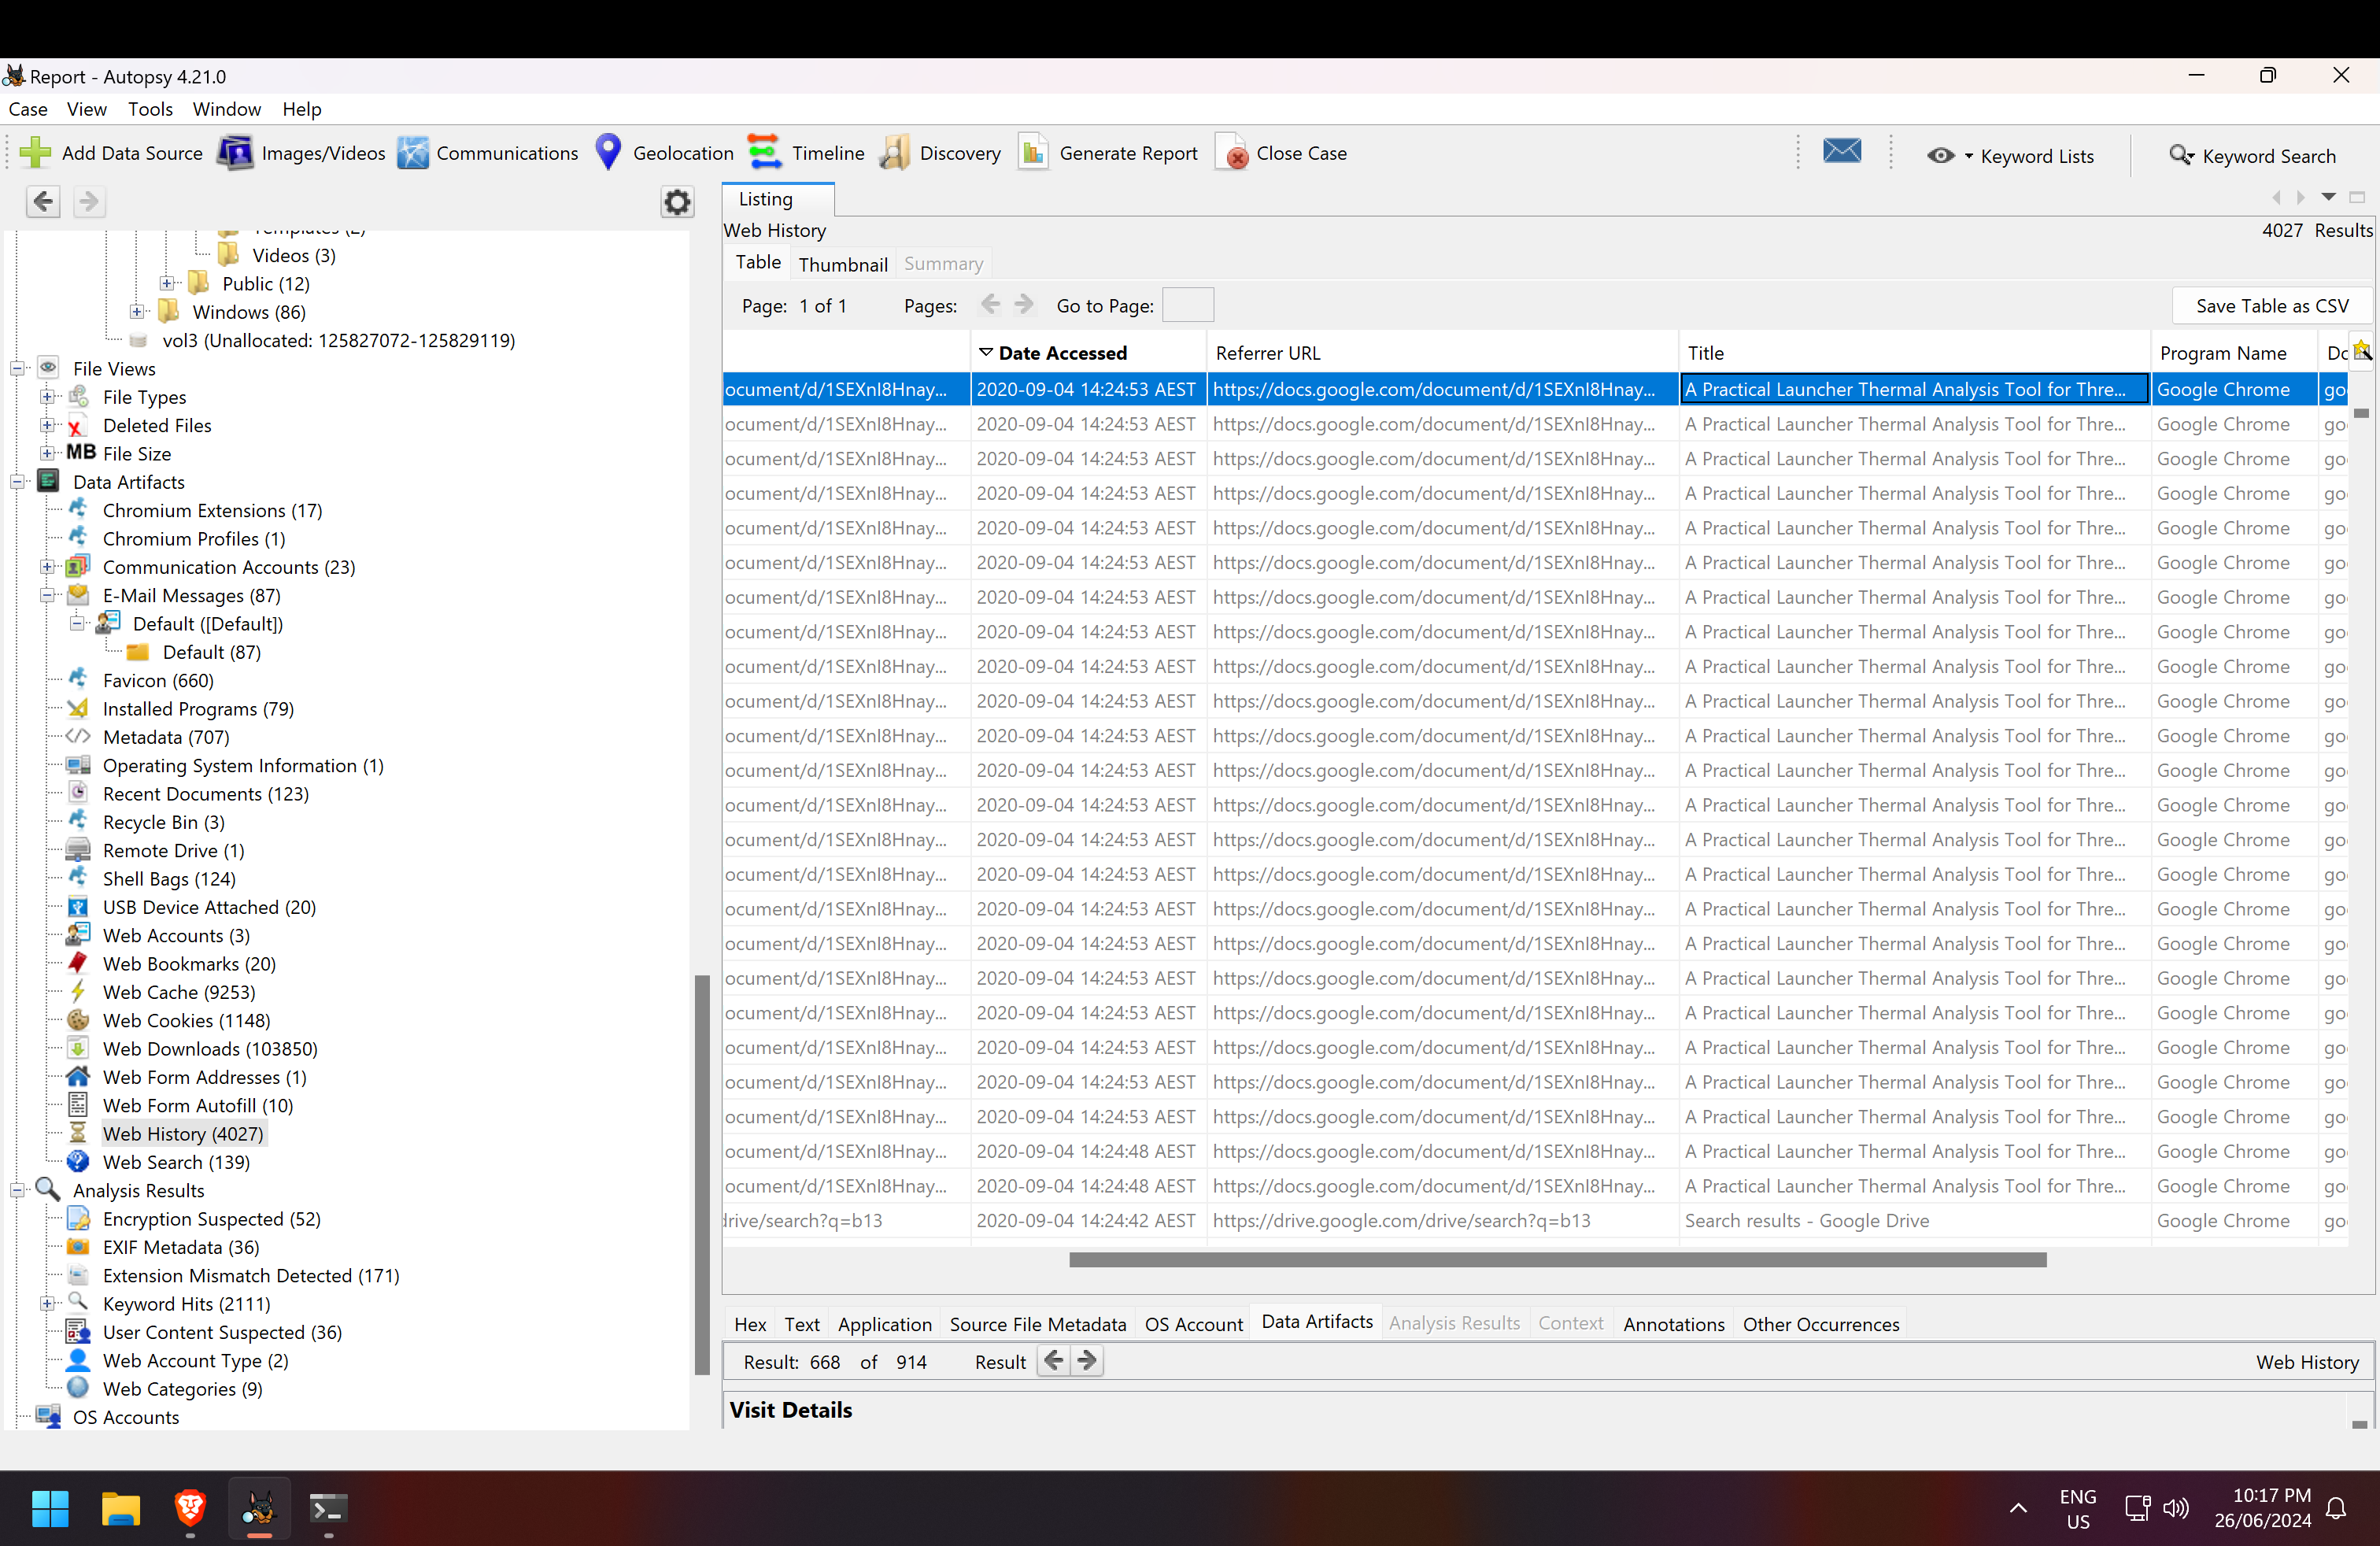
\includegraphics[width=1.0\textwidth]{history3.png}
    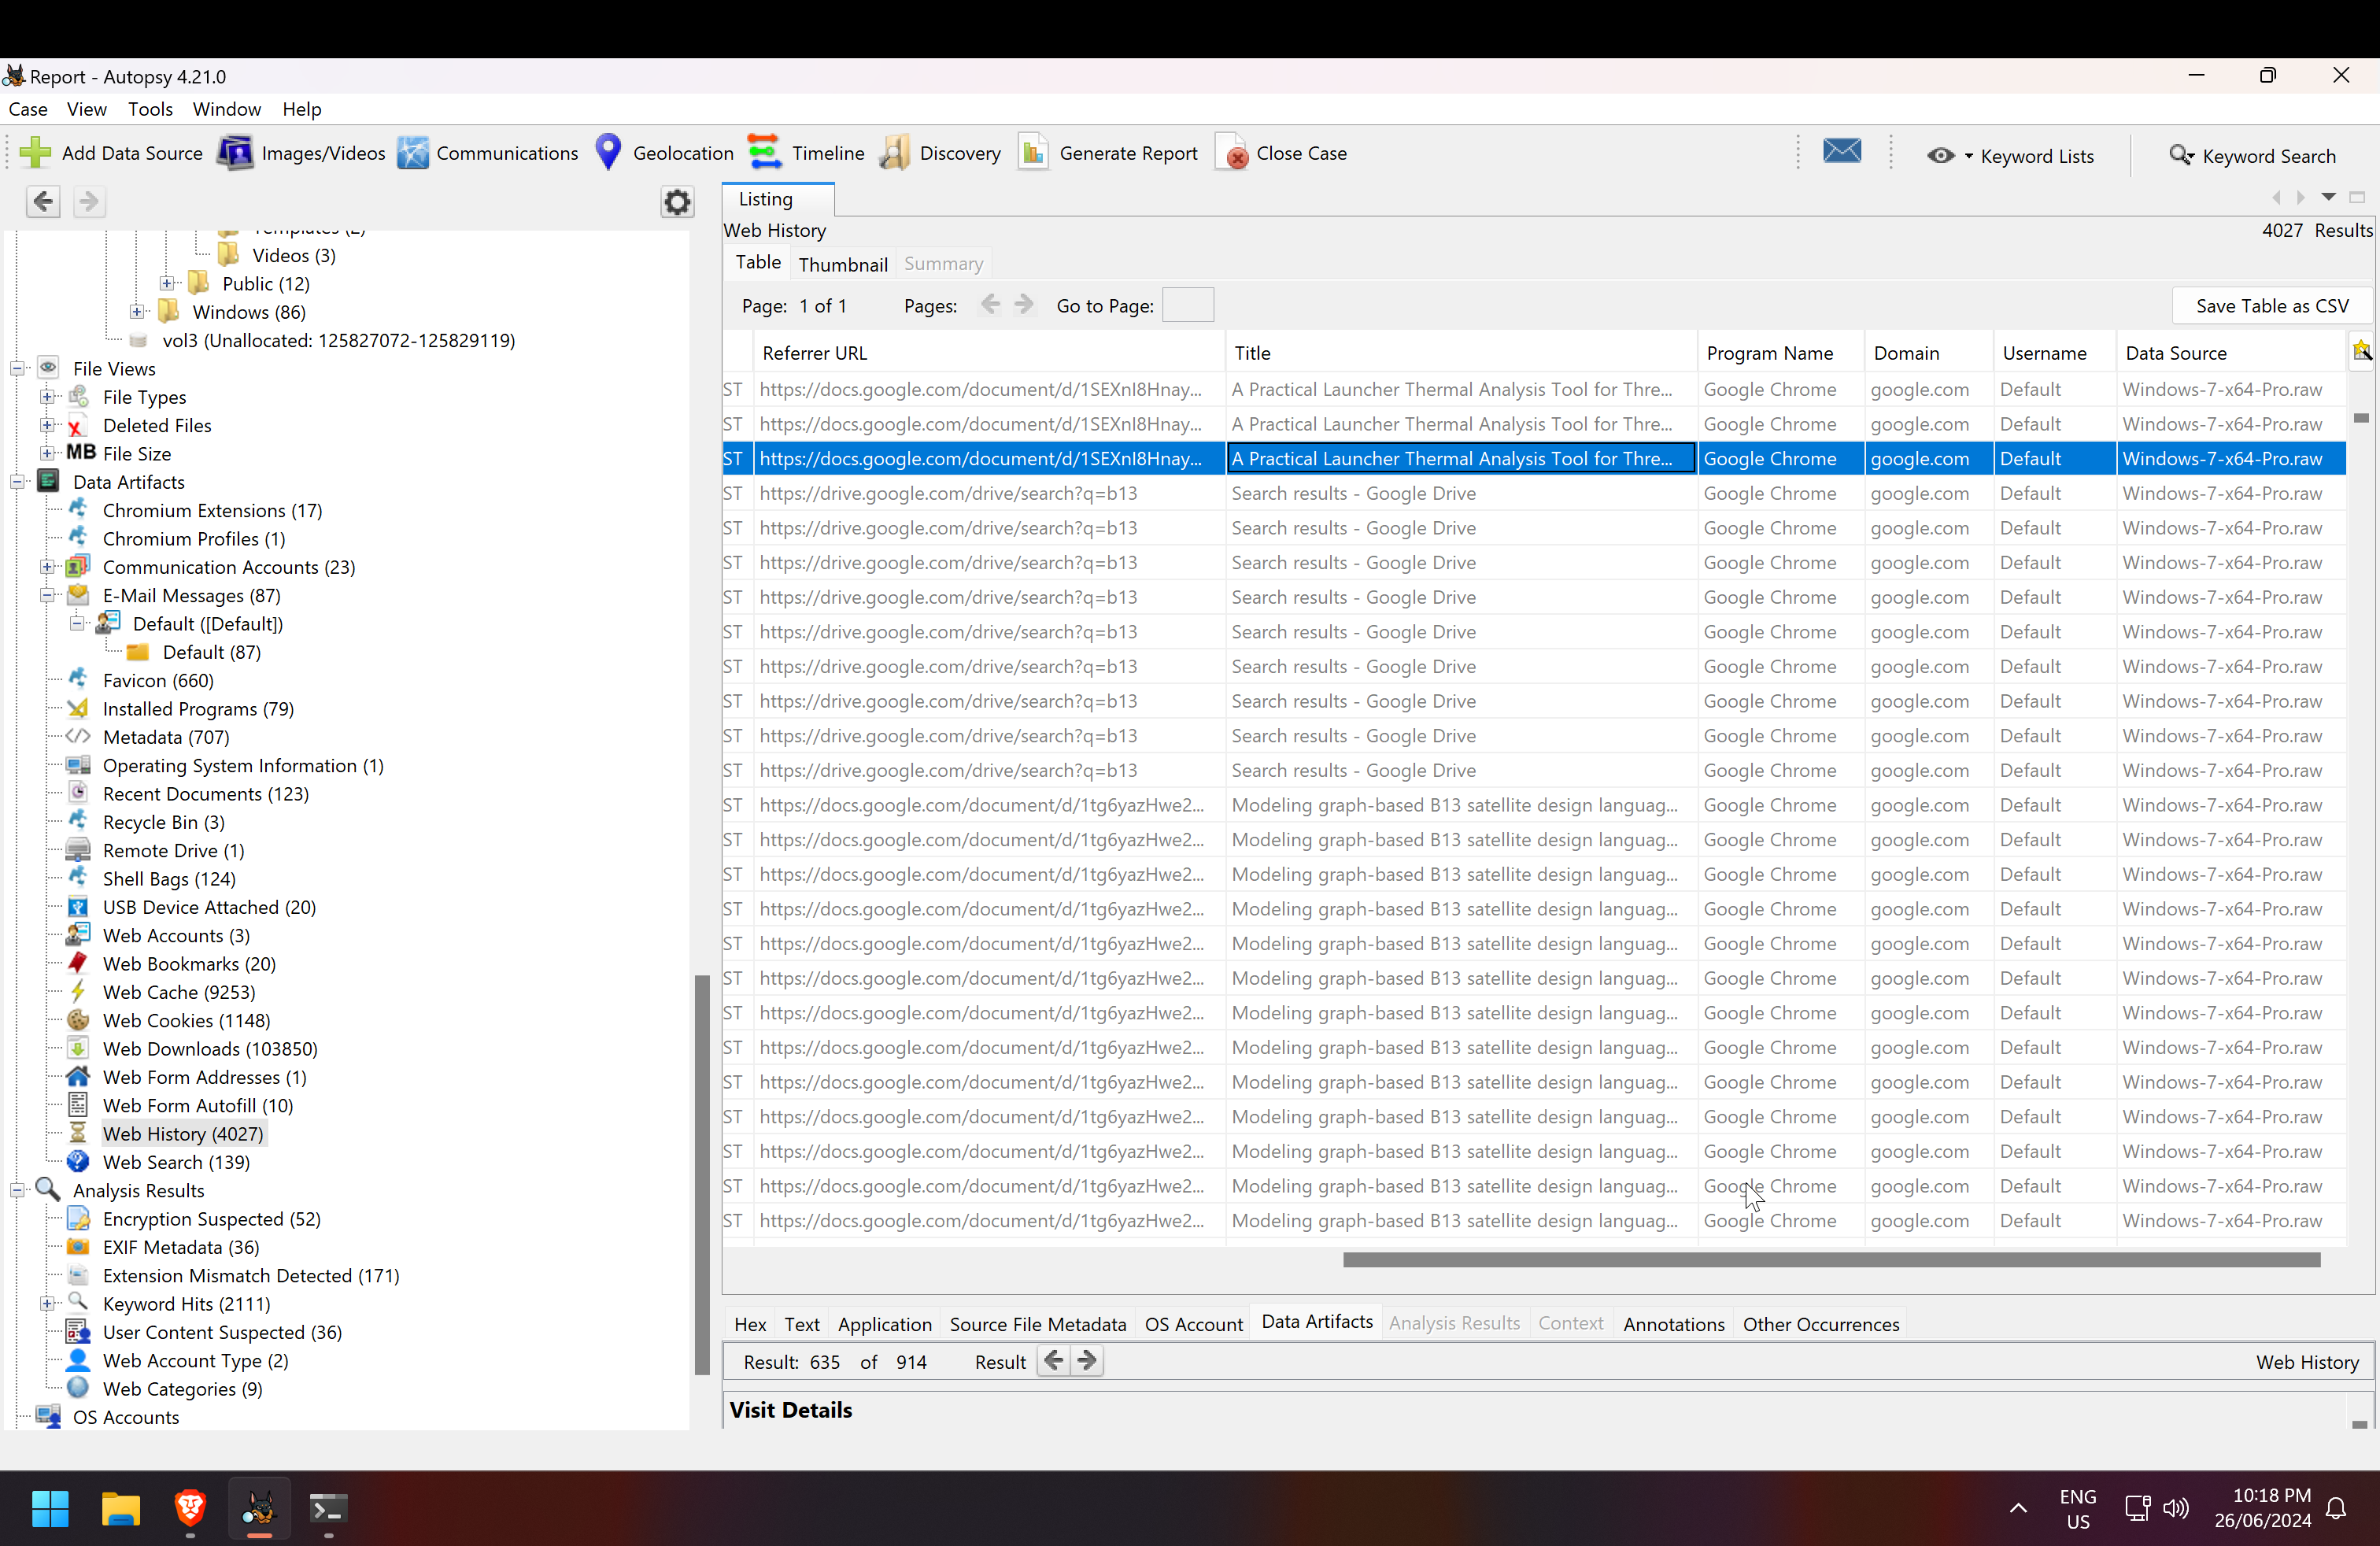
\includegraphics[width=1.0\textwidth]{history4.png}
    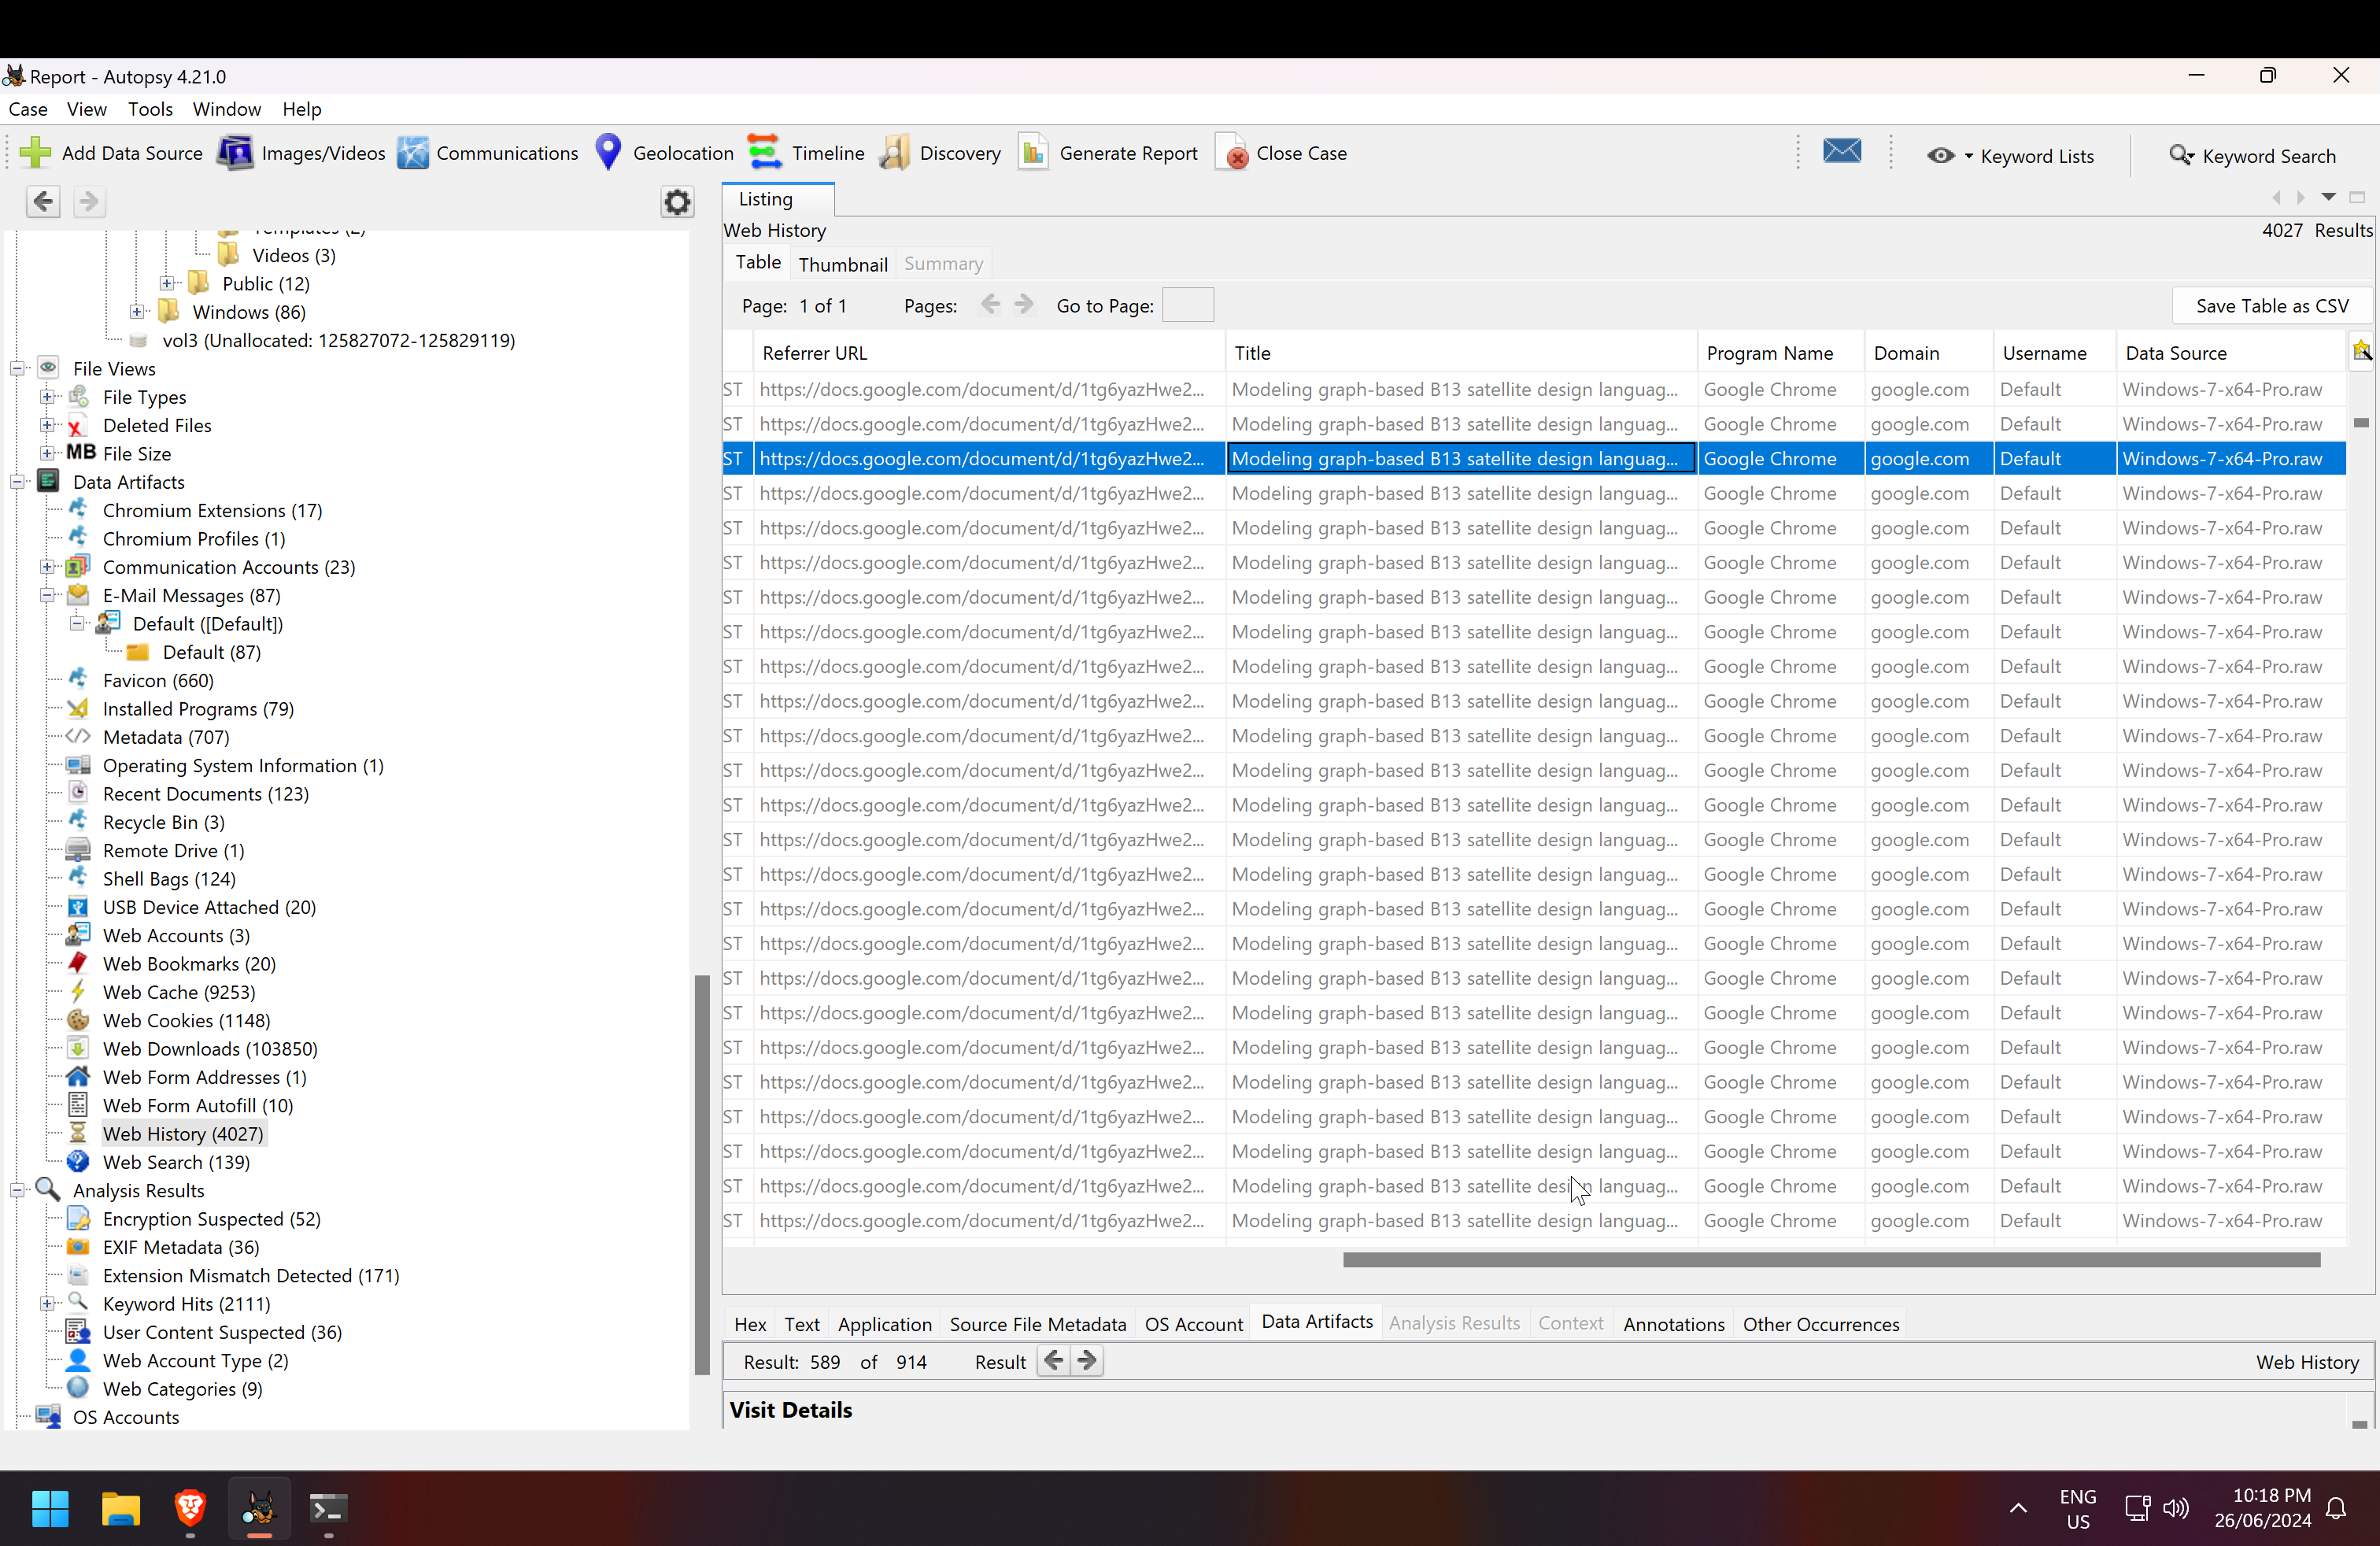
\includegraphics[width=1.0\textwidth]{history5.png}
    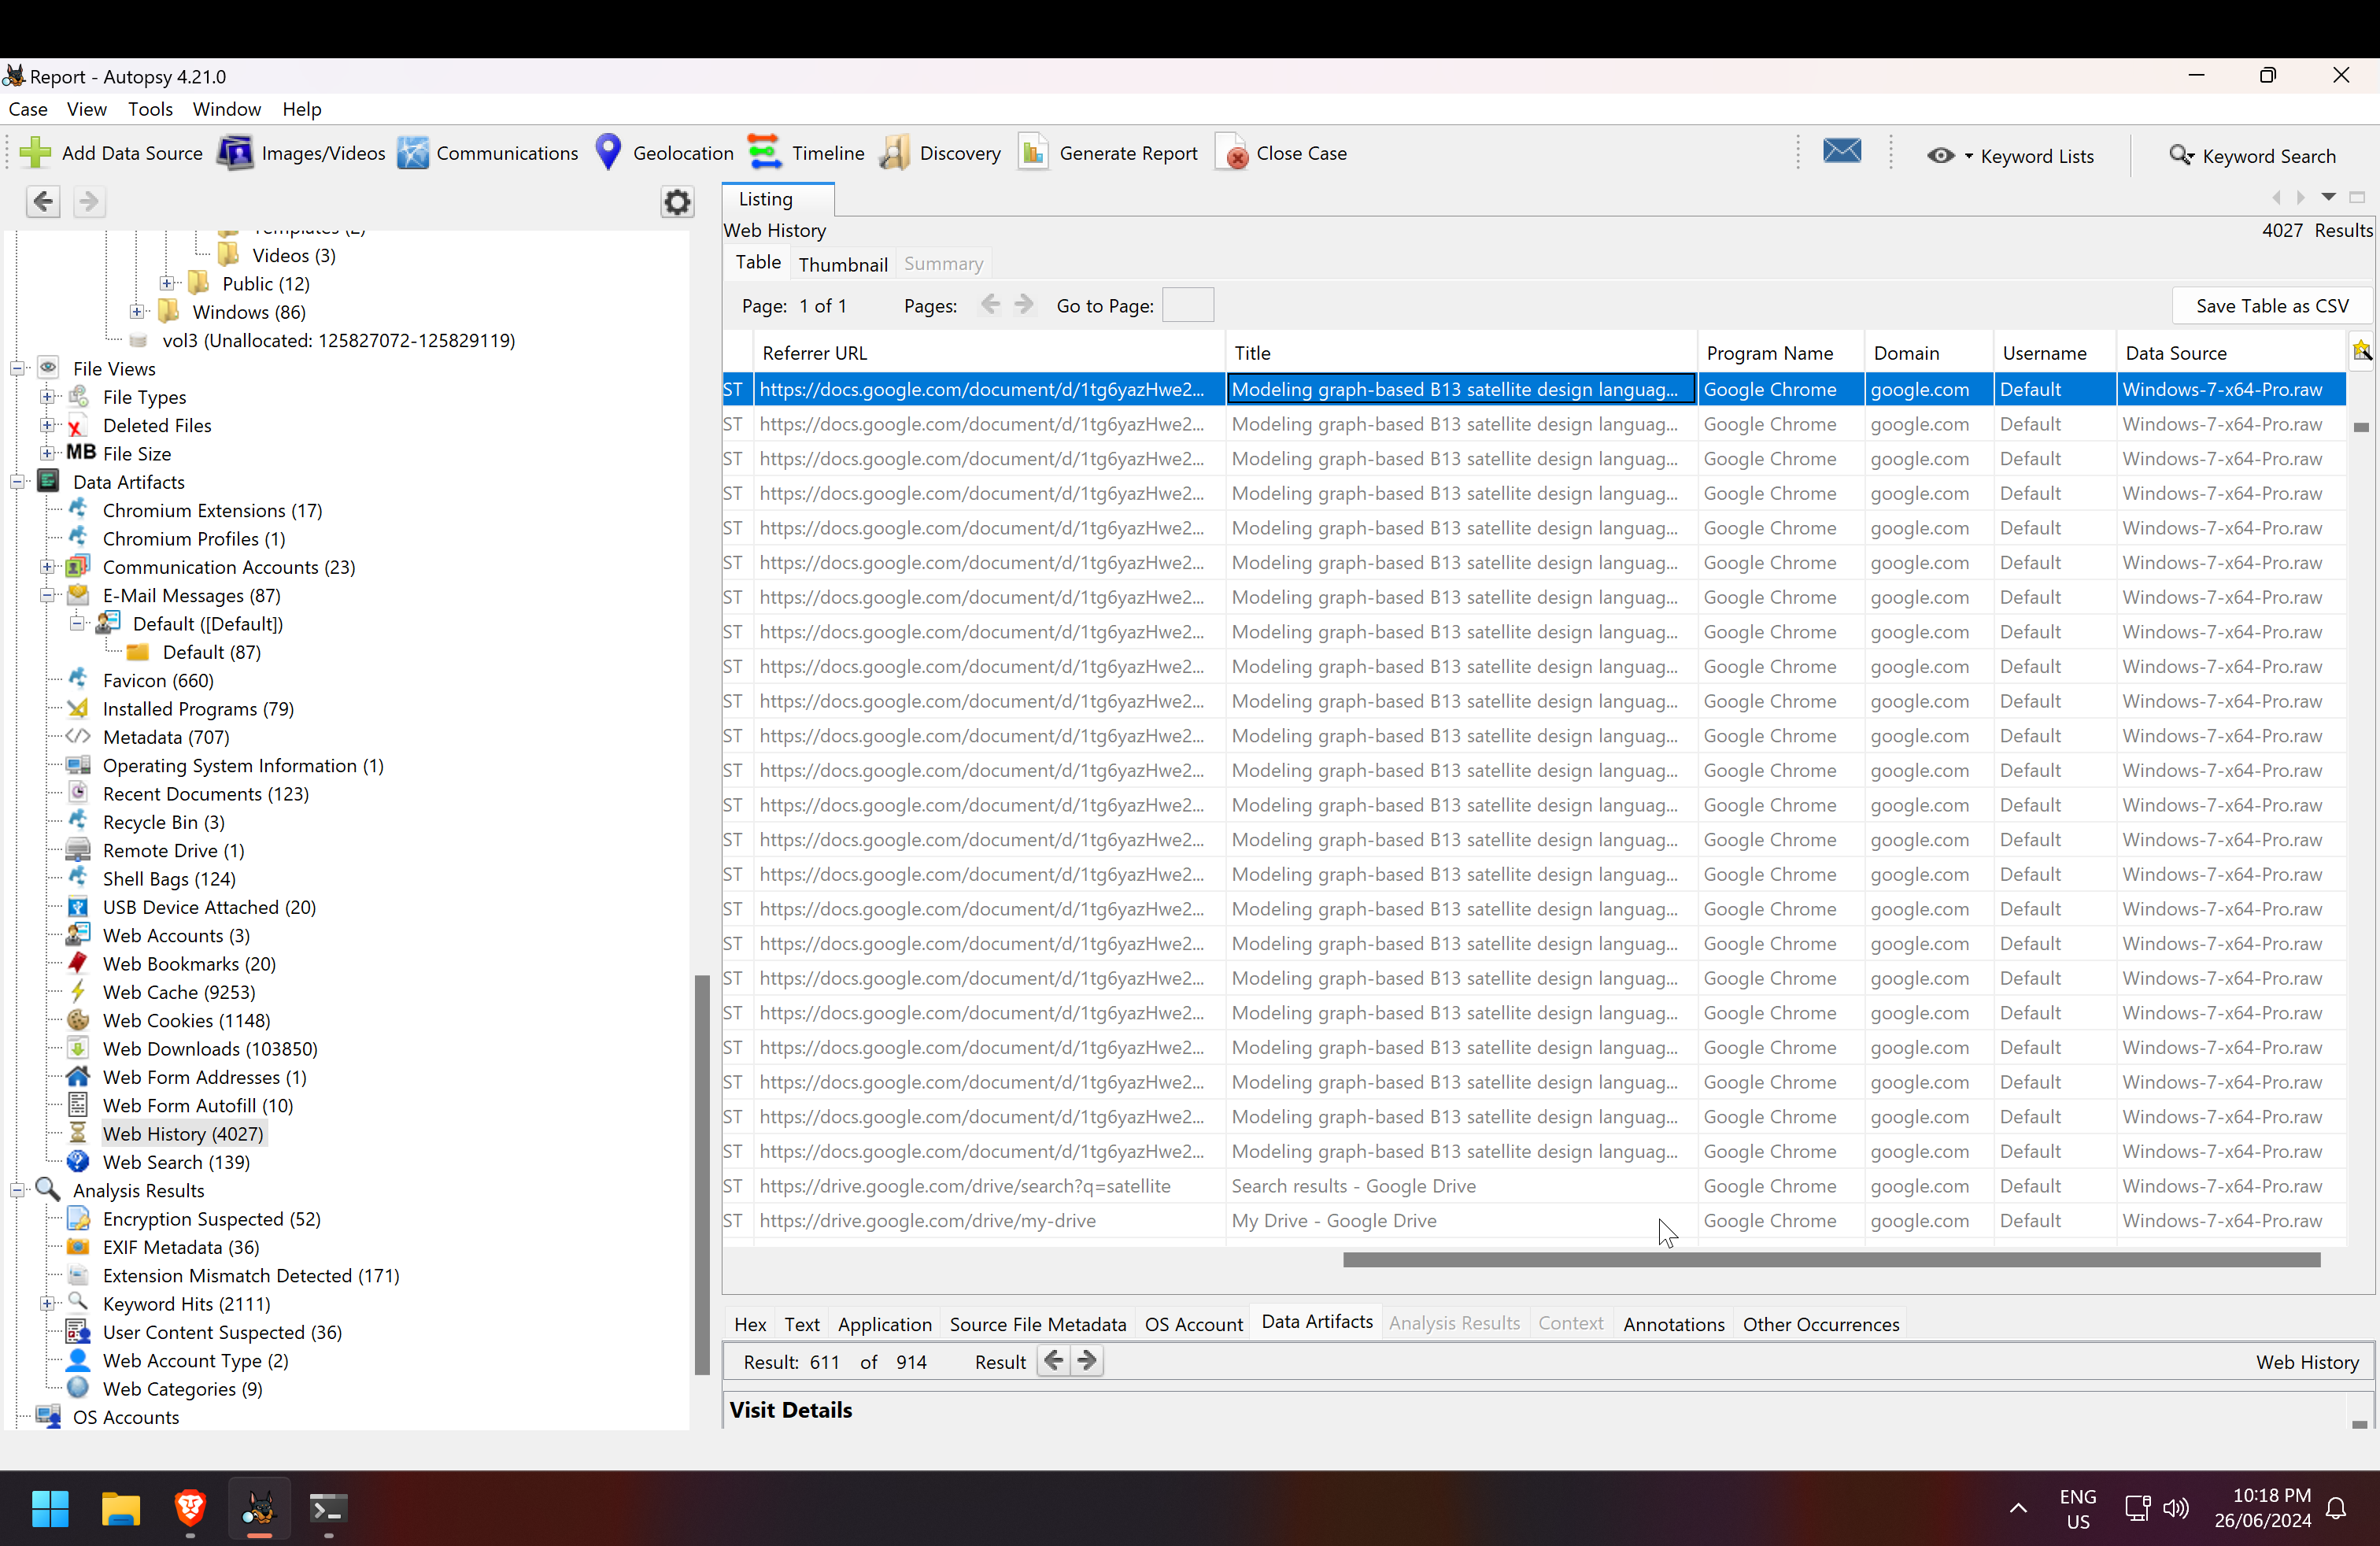
\includegraphics[width=1.0\textwidth]{history6.png}
    \caption{Recent browsing history}
    \label{fig:webhistory}
\end{figure}

\begin{figure}[H]
    \centering
    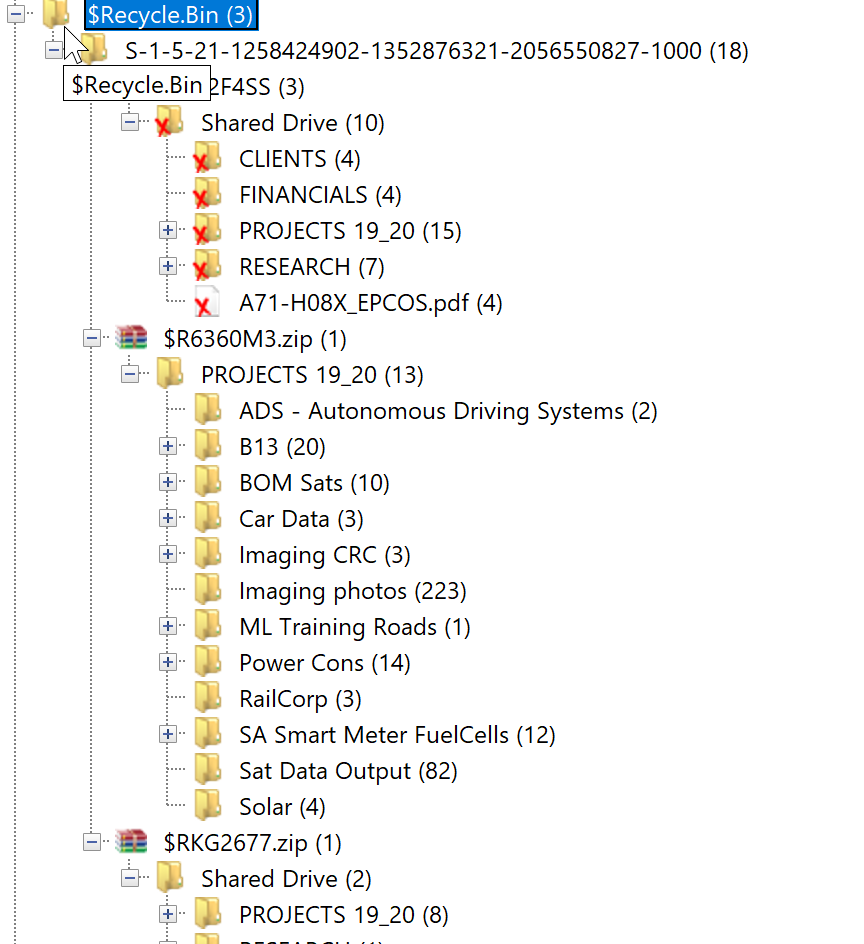
\includegraphics[width=1.0\textwidth]{recycle.png}
    \caption{Recycling bin}
    \label{recycle}
\end{figure}

\begin{figure}[H]
    \centering
    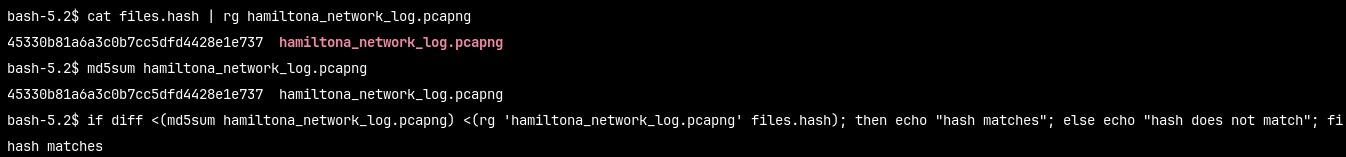
\includegraphics[width=1.0\textwidth]{pcap_verification.png}
    \caption{Cryptographic hash verification of the packet capture file}
    \label{pcap_verification}
\end{figure}

\begin{figure}[H]
    \centering
    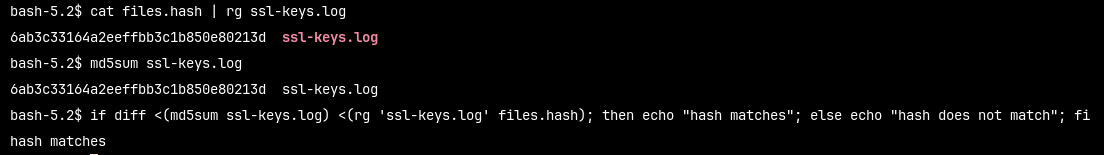
\includegraphics[width=1.0\textwidth]{ssl_key_log_verification.png}
    \caption{Cryptographic hash verification of the SSL key log file}
    \label{ssl_key_log_verification}
\end{figure}

\begin{figure}[H]
    \centering
    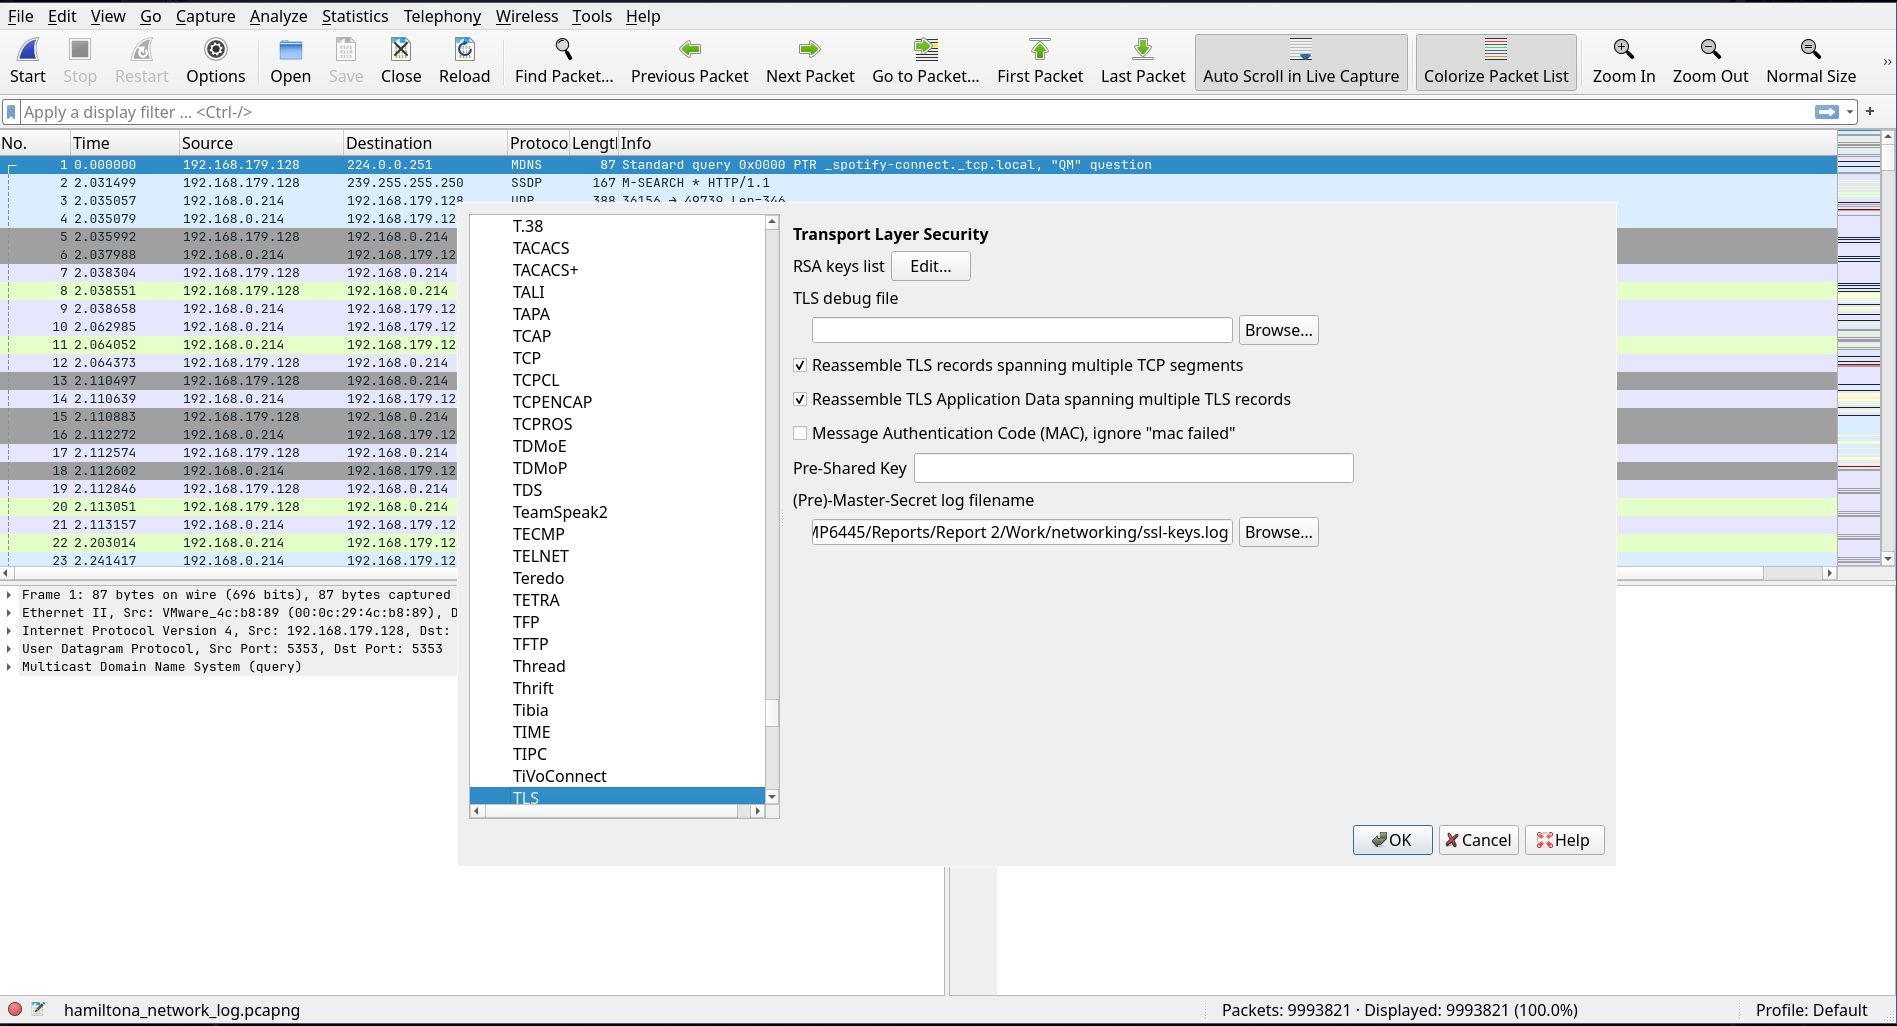
\includegraphics[width=1.0\textwidth]{importing_ssl_key_log.png}
    \caption{Importing the SSL key log to Wireshark}
    \label{importing_ssl_key_log}
\end{figure}

\begin{figure}[H]
    \centering
    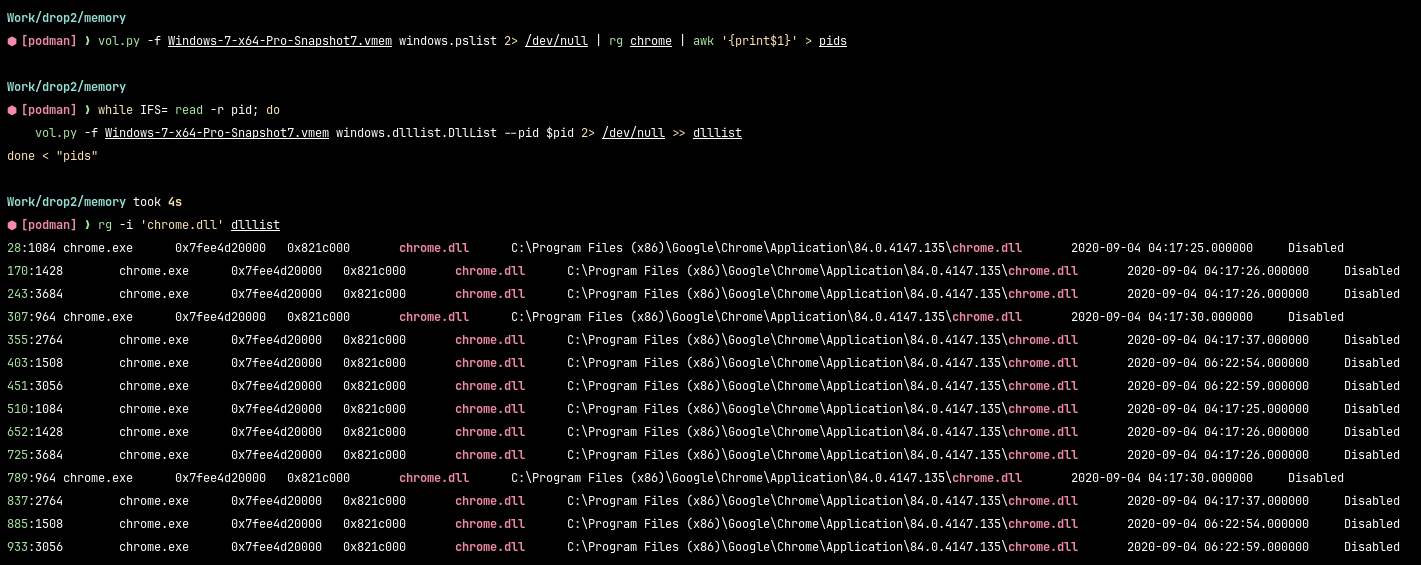
\includegraphics[width=1.0\textwidth]{chrome_version.png}
    \caption{Finding the version of Google Chrome used from the memory dump}
    \label{chrome_version}
\end{figure}

% section Figures (end)

\subsection{Dockerfile for Volatility 3 Environment} % (fold)
\label{sec:Dockerfile for Volatility 3 Environment}
\subsubsection{Dockerfile}
\label{subsubsec:Dockerfile}
\begin{verbatim}
FROM alpine:edge

# Update and install necessary packages
RUN apk update && apk upgrade && apk add --no-cache \
    python3 \
    7zip \
    shadow \
    curl \
    git \
    tmux \
    neovim \
    starship \
    clang \
    zsh \
    bat \
    eza \
    fzf \
    ripgrep \
    fd \
    bind-tools \
    py3-virtualenv \
    termshark \
    traceroute \
    neomutt

# Add a new user
RUN adduser -D COMP6845
RUN usermod -aG wireshark COMP6845
RUN chsh -s /bin/zsh COMP6845

USER COMP6845
WORKDIR /home/COMP6845

# Clone necessary repositories
RUN git clone https://github.com/tmux-plugins/tpm /home/COMP6845/.local/share/tmux/plugins/tpm
RUN git clone https://github.com/zsh-users/zsh-syntax-highlighting.git /home/COMP6845/.local/share/zsh/zsh-syntax-highlighting
RUN git clone https://github.com/zsh-users/zsh-autosuggestions /home/COMP6845/.local/share/zsh/zsh-autosuggestions
RUN git clone https://github.com/Aloxaf/fzf-tab /home/COMP6845/.local/share/zsh/fzf-tab

# Set up volatility
RUN mkdir -p /home/COMP6845/.local/bin
WORKDIR /home/COMP6845/.local/bin
RUN python3 -m venv volatility
RUN ./volatility/bin/pip install --upgrade pip
RUN ./volatility/bin/pip install volatility3

WORKDIR /home/COMP6845
RUN echo "alias 'vol.py'='/home/COMP6845/.local/bin/volatility/bin/vol'" >> .zshrc

# Create Mail directory and copy mbox files
RUN mkdir -p /home/COMP6845/Mail
COPY --chown=COMP6845:COMP6845 Emails/Harris/all.mbox /home/COMP6845/Mail/harris.mbox
COPY --chown=COMP6845:COMP6845 Emails/Hamilton/all.mbox /home/COMP6845/Mail/hamilton.mbox

# Configure NeoMutt
RUN echo 'set mbox_type=mbox' >> /home/COMP6845/.neomuttrc
RUN echo 'set folder=~/Mail' >> /home/COMP6845/.neomuttrc
RUN echo 'mailboxes ~/Mail/hamilton.mbox ~/Mail/harris.mbox' >> /home/COMP6845/.neomuttrc
RUN echo 'set spoolfile=~/Mail/hamilton.mbox' >> /home/COMP6845/.neomuttrc

CMD ["zsh"]
\end{verbatim}

\subsubsection{zshrc}
\label{subsubsec:zshrc}

\begin{verbatim}
# Lines configured by zsh-newuser-install
HISTFILE=~/.histfile
HISTSIZE=1000
SAVEHIST=1000
bindkey -e
# End of lines configured by zsh-newuser-install
# The following lines were added by compinstall
zstyle :compinstall filename '/home/COMP3141/.zshrc'

autoload -Uz compinit
compinit
# End of lines added by compinstall

alias vim=nvim
alias v=nvim

alias cat=bat

alias ls='eza --icons'
alias ll='eza --icons -l'
alias la='eza --icons -la'

# Plugins
source ~/.local/share/zsh/zsh-syntax-highlighting/zsh-syntax-highlighting.zsh
source ~/.local/share/zsh/zsh-autosuggestions/zsh-autosuggestions.zsh
source ~/.local/share/zsh/fzf-tab/fzf-tab.plugin.zsh

# Start starship
# ~/.zshrc
eval "$(starship init zsh)"
\end{verbatim}

\subsubsection{Instructions for use}

Install and set up Docker or Podman. Then:

\begin{enumerate}
    \item Create a new, empty directory and change into said directory.
    \item Copy the contents of Section~\ref{subsubsec:Dockerfile} into a file named \texttt{Dockerfile} in the current working directory.
    \item Copy the contents of Section~\ref{subsubsec:zshrc} intto a file named \texttt{.zshrc} in the current working directory.
    \item Execute the following command to build the container image: \texttt{docker build -t comp6845-report2 .}
    \item Execute the following command to initialise a new container from the image that was previously built and enter it: \texttt{docker run -it --name=COMP6845-Report2 comp6845-report2 zsh}
\end{enumerate}

% section Dockerfile for Volatility 3 Environment (end)


\end{document}
